% po4a: environment longtable {}
% po4a: separator longtable "(?:&|\\\\\\\\|\\\\hline)"


\documentclass[a4paper,oneside,parskip=half,numbers=noenddot]{scrbook}


%%% Page Layout %%%
\textwidth=14.7cm % these two commands make the page fit in a box 
\textheight=22.1cm % ... that works on both letter and A4 paper
%\hoffset=5.8754pt % enable if using letterpaper to center document on page


%%% Preamble things that must happen first %%%


%%% Basic Setup %%%
\pdfminorversion=7 % use a more current pdf version to support better graphics inclusions


%%% Language support %%%
\usepackage[utf8]{inputenc} % use utf-8 encoding for better language support
\usepackage[T1]{fontenc} % uses 8-bit font encoding for better character support
\usepackage{lmodern} % use lmodern font for better character support and a prettier font


%%% Additional Simple Packages %%%
\usepackage{color} % for latexdiff
\usepackage[normalem]{ulem} % for latexdiff


%%% Graphics Packages %%%
\usepackage{graphicx}
\graphicspath{{img/}{./img/}{src/img/}}
\usepackage{wrapfig}
\usepackage{pict2e}


%%% User defined commands and associated packages %%%
\usepackage{comment}
\excludecomment{comment2016}

\newcommand{\unit}[1]{\ensuremath{\, \mathrm{#1}}} % use \unit{km} in math mode for better units

\usepackage{framed}
\newcommand{\oldrule}[1]{} % don't display oldrule (next line is displayed oldrule)
%\newcommand{\oldrule}[1]{\framebox{#1}} % displays oldrule references in a nice box


%%% GitInfo %%%
\usepackage{gitinfo2}
% gitinfo2 package can be found in the dependencies directory
% git hooks must also be installed and these are found in the scripts directory


%%% Tabular environment changes and packages %%%
\usepackage{array} % basic table package, "a must use"
\usepackage{longtable}
\usepackage{multicol}
\usepackage{multirow}

\newcolumntype{P}[1]{>{\raggedright\arraybackslash}p{#1}} % use column type 'P' instead of 'p' for non-justified paragraph text in a table - used primarily in the freestyle judging sections


%%% Additional basic custimizations %%%
\renewcommand{\thepart}{\arabic{part}} % arabic part numbering
\renewcommand{\thechapter}{\arabic{part}\Alph{chapter}} % make chapters numbered with part and then letter
%\renewcommand{\thesection}{\arabic{part}.\arabic{section}} % replace chapter number with part number in sections %% used prior to reorg

\setcounter{secnumdepth}{3} % makes subsubsections numbered

\usepackage[shortlabels]{enumitem} % allows list customization here below
\setlist{itemsep=-1mm, topsep=-1pt, partopsep=0pt} % customize spacing around lists

\newlist{judging_items}{itemize}{1} %redefine itemize for the freestyle judging grid to fit
\setlist[judging_items]{label=\textbullet,leftmargin=*, labelsep=0.7mm,itemsep=-1mm, topsep=-6pt, partopsep=-5pt}


\RedeclareSectionCommands[
  beforeskip=-\baselineskip,
  afterskip=.5\baselineskip]{section,subsection,subsubsection}
% this command is supposed to replace titlesec's titlespacing option
% the desired before/after spacing was {12pt plus 4pt minus 2pt}{0pt plus 2pt minus 2pt}




%%% Customize Part/Chapter/Section/Page numbering %%%
\usepackage{remreset} % allows the resets here below
\makeatletter
\@addtoreset{chapter}{part} % reset chapter numbering for each part
\@addtoreset{section}{part} % reset section numbering for each part
%\@removefromreset{section}{chapter} % don't reset section numbering in new chapters
\makeatother

%don't reset page numbers ever (specifically not after frontmatter)
\makeatletter
\def\pagenumbering#1{%
  \gdef\thepage{\csname @#1\endcsname \c@page}}
\makeatother


%%% Headings %%%
\usepackage[markcase=ignoreuppercase,autooneside]{scrlayer-scrpage} %better headings without uppercase TOC heading
\pagestyle{scrheadings}
\clearscrheadfoot %clear all header and footer styles to allow custimization
\cfoot[\pagemark]{\pagemark} %pagenumbers in footer
\makeatletter
\let\Oldpart\part
\newcommand{\parttitle}{}
\renewcommand{\part}[1]{\Oldpart{#1}\renewcommand{\parttitle}{#1}}
\renewcommand{\chaptermark}[1]{\markboth{#1}{}}
\renewcommand*{\chapterpagestyle}{headings} %display headers on first page of chapters

\chead[]{
  \ifnum\value{chapter}>0
    \thepart \ \parttitle -- \leftmark
  \else
    \thepart \ \parttitle 
  \fi
  }
\makeatother


%%% Hyperref %%%
% must be loaded as late as possible in preamble, with a few things after
\usepackage{hyperref} % clickable table of contents, index in pdf files 
\hypersetup{
    colorlinks,
    citecolor=black,
    filecolor=black,
    linkcolor=black,
    urlcolor=black
}


%%% Must be loaded after hyperref %%%
\usepackage[numbered]{bookmark} % customize PDF bookmarks 
\usepackage{minitoc} % for table of contents per part


%%% TOC custimization %%%
%% all of this comes after minitoc is loaded %%
\setcounter{tocdepth}{-1} % only includes parts and chapters (not sections) in main TOC
\mtcsetdepth{parttoc}{1} % only includes chapters and sections (not subsections) in part TOCs

\usepackage[tocindentauto]{tocstyle} % prettier TOC
\usetocstyle{allwithdot} %use 'KOMAlike" if you don't want dots
\settocstylefeature [-1] {entryvskip} {15pt}
\settocstylefeature [0] {entryvskip} {10pt}
\settocstylefeature [0] {entryhook} {\hspace{18pt} }

\renewcommand{\mtcgapbeforeheads}{0pt}
\renewcommand{\mtcgapafterheads}{0pt}
\mtcsettitle{parttoc}{Contents} %renames the part TOC to match main TOC

\usepackage{tocloft} % package for below command
\renewcommand{\cftsecnumwidth}{3em} %changes spacing between number and name on sections in TOC (and minitocs) to help with long section numbers (i.e. 1C.14)


\begin{document}
\begin{titlepage}
\centering
\ \\
\vspace{5cm}
{\Huge 2015 Competition Rulebook}
\vspace{5mm}


\includegraphics{iuf-logo}

\vspace{5mm}
{\huge International Unicycling Federation}

\vspace{5mm}
{\Large Preliminary Version \quad May, 2015}

\vspace{55mm}
Prepared by the IUF Rulebook Committee.

\vspace{5mm}
{\small Copyright \copyright\ 2015 by the International Unicycling Federation, Inc. All rights reserved.}
  \small{Revision: \gitHash, \gitCommitterDate}

\end{titlepage}

\doparttoc
\tableofcontents

\mainmatter
\part{General Rules and Definitions}
\parttoc

\chapter{General}

\section{Scope of Rules}

\begin{framed}
Mary and I think that this section could be clarified by splitting out scope, use for national events, how to get approval for unicon qualification, and how the rules can be modified.
\end{framed}

\oldrule{1a}
This rulebook is intended to govern all unicycle competition sanctioned by the International Unicycling Federation, and can be used as a guideline for other competitions.

\textit{
The major sections are described in the table of contents at the beginning of this document.
Various charts and forms that supplement these rules may be published separately. 
}

\subsection{Unicon}

\oldrule{1.1}
All IUF Unicons (International Unicycling Conventions) must abide exclusively by these rules.
Further rules may be added to cover specific situations, but they may not override the IUF rules without prior approval by the IUF Board of Directors.
All additional rules must be published well in advance of international competition, and published together with registration forms.

\subsection{Other Uses for These Rules}

\oldrule{1.1}
National or local unicycling organizations may have their own rules.
Though they may use IUF rules as a basis for their own rules, in national or local competitions, those rules can no longer be called IUF rules.
To get proper results for Unicon qualification it is needed to follow the IUF Rulebook as described above.

Any national organization that wishes to get its modified rules approved by the IUF for a national competition must submit a proposal to the IUF Executive Board at least 90 days before the start of the given event.
If approved, the national competition can still be recognized as an official IUF event.

To host an ``official IUF event'' means that the results of this event are comparable with results from other official IUF events and can count for possible qualification restrictions.
Rules, which are approved for use at a national or local competition by the IUF Board to be used, must not be referred to as IUF rules to prevent confusion for the riders.

\section{How to Use This Rulebook}

\oldrule{begin new}

This IUF Rulebook is organized by competition event.  Each event chapter includes a overview, competitor rules, officials rules, and organizer rules.  Additionally, Chapter 1 covers general rules, not tied to a particular event. 

How you approach the information in this rulebook will depend on what role you play.  The information has been organized with a goal toward separating rules by role, so that you can safely ignore sections that do not pertain to you.  For example, if you are only interested in muni as a competitor, you can ignore other event chapters and you can mostly ignore the officials and organizer rules within the muni chapter.

The following table gives some guidance for what information you need for various roles:

\begin{longtable}{|l|p{8cm}|}
\hline
\textbf{Role} & \textbf{Applicable Sections} \\
\hline
competitor & Chapter 1 and the overview and competitor rules for your events\\
\hline
official & Chapter 1 and the overview, competitor rules, and officials rules for the event you will officiate\\
\hline
event director & Chapter 1 and all sections of the chapter for your event \\
\hline
host & All sections of the rulebook\\
\hline
\end{longtable}

\oldrule{end new}

\section{How the Rulebook is Updated}

\oldrule{1.1.1}
This publication should be updated after every Unicon.
The IUF Rulebook Chair will head the committee, but may optionally name a sub-committee.
The Rulebook Committee will officially start meeting at the close of the Unicon, though the Chairperson can open it before, to take advantage of having so many persons physically together.
The Committee should finish their business and make their specific proposals within three (3) months of the close of the Unicon.
If they need more time, they may ask the IUF President for a time extension.
This is meant to be the only time that changes to the Rulebook are made, although exceptions are possible in extraordinary cases.
The IUF President is responsible for making sure that the Rulebook committee stays focused and on schedule.

Anyone may submit a potential change to IUF Rulebook at any time.
These will not be official proposals, but suggestions for potential topics during the next Rulebook session.
A forum will also be provided to discuss potential changes throughout the year.
The Rulebook Committee voting time frame and official members of the Rulebook Committee, however, will still be determined by the IUF Rulebook Committee Chair and the IUF Executive Board.

\section{World Champions}

\oldrule{1.8}
The Male and Female winners of each individual event at Unicon are the World Champions for that event. 
There is no age limit to winning the overall title.

Age group winners can use the title `Age-Group Winner', and the term `World Champions' generally refers to winners of Overall, Finals or Expert class. 
See also section \ref{sec:freestyle_world-champions}.

\oldrule{6.12}
Winners in the Expert category at of each event at Unicon are the \textbf{World Champions}.
In the individual events, separate titles are awarded for male and female.
Winners in the Jr. Expert category at Unicon are the \textbf{Junior World Champions}.

\oldrule{7.12}
The male/female winner of the Expert category at Unicon is the Male/Female \textbf{World Champion}.
The male/female winner of the Junior Expert category at Unicon is the Male/Female \textbf{Junior World Champion}.
In the absence of any of these categories, no title will be awarded.
No title is awarded for the Advanced category.

\section{World Records, IUF Records}

\oldrule{1.9}
The host should ensure that the competition conditions are conducted and recorded according to the IUF Rulebook and the IUF World Record standards.
If world record standards cannot be used, then the competition results cannot be used for new world records.

\section{Ownership of Data}

\oldrule{1.10}
Each Unicon or other large unicycling convention is a piece of history.
At the conclusion of a Unicon or other international event, or within one month thereafter, the convention host must supply the IUF with a list of competition and other results.
This list will include all data collected to determine placement and winners at all levels and in all events held at the convention.
This data is considered public, and is not the sole property of the host.
Copies of attendee registration details, judging sheets, protest forms, and related paperwork are not necessarily public, but are the shared property of the host and the International Unicycling Federation, and must be made available upon request.
If the host wishes to discard any of this paperwork or data, it must be turned over to the IUF, not thrown away.
If requested, the host and convention officials must also provide further information, not necessarily in writing, about decisions made, methods used, and other details covered in the process of planning and running the convention.
This information can be invaluable to future hosts, and must not be hidden or lost.

\section{Hierarchy of Officials}

\oldrule{1e}
These people make the competition events work.
All of the tasks detailed below must be covered for the events to work.
Names must be assigned for all the jobs listed below, to create a hierarchy of authority for the convention.
All officials are expected to work objectively and impartially.

\subsection{General Officials}

\oldrule{1.27}
\textbf{IUF Board Of Directors:} The IUF Board represents the interests of the IUF on convention requirements, both in the area of competition rules and the necessary spaces and facilities for them, and for any other requirements that go along with putting on an IUF convention.
If problems arise in meeting the IUF requirements, the IUF Board and Convention Host work together to find solutions or compromises.
The bulk of this should happen during the early planning stages for a convention, when facilities and schedules are being assembled.

\textbf{IUF Convention Liaison:} The Liaison is an optional person who can represent the IUF Board when communicating with convention hosts.
The Liaison essentially has the same powers as the IUF Board, but must report to the IUF Board and take direction from it.

\textbf{Convention Host:} This is a single person, or a collective group, that has made the commitment to host a unicycle convention using IUF rules and guidelines.
By agreeing to host an IUF convention, they also agree to follow those rules and guidelines wherever possible.
If known problems arise in the arrangement of facilities, schedules and events, the Host and the IUF will work together to resolve the problems.
For the most part, the Convention Host is the ultimate authority for what happens, and does not happen, at the convention.
The exception is any IUF requirements for convention facilities or contents, and rules for IUF competition events.

\textbf{Top Competition Officials:} The Race Director, Referee, Artistic Director and Chief Judge are the positions of authority for racing and artistic events, respectively.
They are not autonomous, and must answer to the Convention Host.
It is highly recommended that none of these jobs be combined, and that there be at least one separate person for each.

\begin{framed}
The top officials needs to be reworded to include other events.
\end{framed}

\chapter{Competitor Information}

\section{Personal Responsibility}
\oldrule{1.24}
All attendees should remember that they are guests of the convention hosts, and ambassadors of our sport to all new riders, visitors from far away, and to people in the hosting town.
Remember that the Host is renting the convention facilities, and attendees are expected to treat them well.
Each rider is responsible for the actions of his or her family and non-riding teammates.
Riders may lose placement in races, risk disqualification from events, or be ejected from the convention if they do not work to minimize disruptions from these people.

\section{Supervision of Minors}
\oldrule{1.24}
A parent, guardian or other designated person, must supervise all minors.

\section{Knowing The Rules}
\oldrule{1.25}
Lack of understanding of rules will be at the disadvantage of riders, not officials or the IUF.
The IUF is also not responsible for any errors that may occur in the translation of rules and information into languages other than those in which they were originally written.

\section{Your Privilege}
\oldrule{1.26}
Entry in the competition is your privilege, not your right.
You are a guest at the Host's event.
You may be in an unfamiliar country, with different customs that are considered the norm.
The Host and convention officials determine whether certain events, age groups, or policies will be used.
As an attendee, you are obligated to obey all rules and decisions of convention officials and hosts.

\section{Nations Represented}
\oldrule{1.21}
For events where the number of participants is limited by country, there may be some question of what country a rider, pair or group may represent.
Riders must represent the country in which they hold citizenship, or in which they are a legal resident.
For example, if a rider is attending school in a different country, and is in that country legally, the rider can either represent that country or the rider's home country.

If necessary, citizenship or residence may be established with a passport, driver's license, or legal ID for the country the rider wishes to represent.
Riders on extended vacation, exchange students, and other temporary residents of other countries are not eligible to represent those countries, except in multi-rider events (see below).

For Pairs Freestyle or other two-person events, the pair can represent any country that either rider is eligible to represent.

For Group Freestyle, sports teams or other multi-rider events, the group must represent the country that the greatest number of the group's riders is eligible to represent.
If there is a tie in this number, the group can represent either of the tied countries.

\chapter{Host Information}

\section{Convention Aspect}

\oldrule{1.2}
All competitions at a Unicon need to make every effort to have equal time for the convention side of Unicon by involving as many competitors as possible and making the event spectator-friendly for other Unicon participants as well as non-unicyclists.
Any of the following are examples to achieve this goal:
\begin{itemize}
  \item Workshops related to the event
  \item Fun competitions based on the event
  \item Instant results for the spectators
  \item Ways for other competitors to be introduced to the event
  \item Entertainment during breaks in the competition (such as half time entertainment)
  \item Schedule of the events posted in multiple places
\end{itemize}

\section{Required Events}

\begin{framed}

This section used to be called Host's Option-Unicon.
\end{framed}

\oldrule{1.3}
Unicon should include at least one event from each of the following event groups. 
Hosts are free to add events, age groups or variations that do not appear here, as long as there is no conflict with the existing rules. 
When in doubt contact the IUF Rules Committee.
\begin{itemize}
  \item Track Racing: the required races from section \ref{sec:track-field_minimum-racing-events}.
  \item Other Racing: Road, specialty/novelty races; see section \ref{sec:track-field_alternate-optional-fun-events}.
  \item Team Games: Unicycle Hockey, Unicycle Basketball. See chapters \ref{part:hockey} and \ref{part:basketball}.
  \item Field events: Long Jump, High Jump, Gliding/Coasting. See chapter \ref{part:jumps} and chapter \ref{part:track-other}.
  \item Non-competition events: workshops, fun games, sightseeing rides, muni rides.
  \item Artistic events: Freestyle, Standard Skill, Flatland, Street; see chapters \ref{part:freestyle}, \ref{part:standard}, \ref{part:flat}, and \ref{part:street}.
  \item Muni: Cross Country, Orienteering, Uphill, Downhill, Trials; see chapter \ref{part:muni} and chapter \ref{part:trials}.
\end{itemize}

\section{Sponsors}

\oldrule{1.3.5}
The convention host has the option to seek and obtain private sector sponsorship; for example The Unicycle.com Freestyle Awards, the Coca-Cola Hockey Cup, etc. 
This will allow opportunities for external funding to defray costs for host organizations and competitors. 
Sponsors are limited to organizations that would not bring the IUF into disrepute and are consistent with the aims and objectives of the International Unicycling Federation, Inc.

\section{Materials \& Equipment}
\oldrule{1.19}
The Host must supply all necessary materials and equipment to run the competitions, such as a timing system, starting posts, cones for the IUF Slalom, etc.
Other materials such as paper and writing materials, judging tables, printers, basketballs, hockey sticks, etc. are also necessary.

\section{Early Announcement of Rule Changes}
\oldrule{1.4.1}
For international competitions, written rules are needed for any planned events not described in the IUF Rulebook, and for events where additional rules are required. 
These special rules could be variations on the optional events found in this Rulebook. 
Such rules should be published at the same time as registration forms, or earlier, and must be published at least one month before the start of the event. 
These rules can be published along with registration forms, and/or on the convention web site. 
Competitors need to know the specific rules so they can train for those specific events! 
Hosts also need to decide on rules early, so there is less to worry about near competition time. 
Rule changes may be a necessary reality, for reasons such as changes in venue, weather or available equipment. 
When this happens these changes must be posted to the convention web site immediately. 
Examples: Dismount rules or timing details for off-track races, obstacle information for Street Comp, planned age divisions or combination awards.

\oldrule{1.6}
If competition events or games not found in the IUF Rulebook are planned, written rules must be provided. 
These rules, if not pre-existing, should be published at the time of announcement of those events. 
This generally means at or before the posting of registration forms. 
For competitors to properly train, and be on an equal footing with local riders, all must be aware of the rules to be used.

\section{Registration Forms}
\oldrule{1.12}
Because of the various options available to riders in different events, riders may enter different events in different age groups.
A properly structured registration form is essential for making these choices clear to the participants.
For example, a rider may enter Pairs as an Expert with an older rider, but may wish to compete in Individual Freestyle in his or her own age group.
Before publishing, a Unicon registration form should be examined and approved by members of the IUF Rules Committee or Board of Directors.
No rider may enter any event until his or her registration form has been completed, including payment and completion of waivers and/or signatures.
No minor may compete until a parent or legal guardian has signed his or her release.

\section{Combining Age Groups}\label{subsec:general_host's-option-unicon_combining-age-groups}}

\oldrule{1.3.2}
In a competition with more than 50 riders, six riders are needed to complete an age group.
In competitions with less than 50 riders, six in each age group are still highly recommended, however three riders are the minimum to complete an age group.
Riders generally enter all events with their age group except for events similar to artistic competitions where there are Junior Expert and Expert categories.

The convention host must combine age groups with less than six riders (three riders for smaller conventions) if needed.
This means that published age groups are not guaranteed.
This can be done on a per-event (= per-discipline) basis.

When combining, combine the smallest age group (that is, the age group with the smallest number of participants) with its smallest neighboring age group (either up or down).
If more than one age group is the smallest, choose the age group with the smallest neighbor for combining.
Continue this process until all resulting age groups (combined and/or original) have at least the minimum required/recommended number of participants.
Male age groups are never combined with female age groups.

\section{Awards}

\oldrule{1.3.3}
The type, number, and quality of awards are the choice of the convention host. 
Because awards are paid for out of the convention budget, the host may determine the amount and level of those awards. 
Generally there are trophies for``top'' events, medals for ``sub-top'' events, and ribbons or certificates for lower events or places. 
The IUF has most frequently awarded 1st-3rd place in most events, but this too is up to the convention host.

\section{Safety Equipment}

\oldrule{1.3.1}
\textit{You will find the detailed rules about safety equipment in each chapter as point x.3 (2.3, 3.3, 4.3 etc.).}
Safety equipment worn by riders must meet the definitions for each, which are found in chapter \ref{chap:general_definitions}.
Hosts may only deviate from these rules for safety equipment if this is inevitable.
The status of ``inevitable'' has to be documented and must be approved by the IUF executive board. 
Any deviation from the IUF safety equipment requirements must be approved and announced at least two months before the event.
Additional inevitable changes that arise just before or during an event cannot be approved by the event director alone.
The approval of two IUF representatives is required in addition to the event director's approval.
These changes are once again only allowed in the case of the inevitable, and not, for example, due to the wishes of the competitors or judges.

\section{Protests}

\oldrule{1.3.4}
Private videos are generally forbidden as a means of verification in case of a protest. 
The host can decide to make an official video of some competitions (for example at the 5-meter-line of the 50 m one-foot race), which has to be announced before the competition to let the competitors know about their option to protest through this video.

\section{Protests}
\oldrule{1.11}
An official protest/correction form must be available to riders at all times.
All protests against any results must be submitted in writing on the proper form within two hours after the results are posted, unless there is a shorter time specified for certain events (for example: track racing).
The form must be filled in completely.
This time may be extended for riders who have to be in other races/events during that time period.
Every effort will be made for all protests to be handled within 30 minutes from the time they are received.
Mistakes in paperwork and interference from other riders or other sources are all grounds for protests.
Protests handed in after awards have been delivered will not be considered if the results have been posted for at least three hours before the awards.
If awards are delivered before results are posted, it is recommended to announce the schedule of posting and the deadline for protests at the awarding ceremonies.
All Chief Judge or Referee decisions are final, and cannot be protested.

\section{Open Practice Area}
\oldrule{1.18}
For Unicon and other large competitions, at least one area with a smooth safe riding surface, sheltered from the weather, must be made available for all or part of the day on most or all days of the convention.
These areas are to be used for non-competition events such as workshops, skills exchange and free practice.

\section{Program Book}

\oldrule{1.13}
At Unicons, all registrants shall be provided with a package of pre-printed information containing a full schedule of all events, maps and directions to all event locations, and as much rule and background information as possible.
This information shall be provided when registrants first check in at Unicon.
Unicon organizers should consider placing as much of this information as is practical in an official Program Book.
This can make excellent reading for family members and spectators, and gets them more involved in our sport.
It's also a great place to sell ads as a source for convention revenue.
At other unicycling events, it is recommended that pre-printed information be provided to all participants.

\section{Availability of Rulebook}
\oldrule{1.20}
The host must make sure there are plenty of copies of the rulebook for officials to study on the spot.

\section{Photography and Videography}
\oldrule{1.5}
The following rules are required for Unicon and are highly recommended for other large international competitions.

In events with closed perimeters, it may be necessary to limit the number of photographers and filmers (hereafter called ``shooters'') allowed inside.
We want great documentation of the events, but not at the expense of safety, and of spectators' ability to see as well.

The following guidelines apply:
\begin{itemize}
\item Shooters must either register ahead of time to be inside the perimeter of an event, or have actual press credentials (professional photojournalists, TV news people, etc.).
\item Registered shooters must have some form of ID given to them, whether it be a pass on a lanyard, a volunteer shirt, or something else to help identify them.
\item The Referee or Head Official for the event has the final say on shooting that can affect the riders and/or spectators’ view.
\item The Referee or Head Official should appoint a Media Manager to manage this task.
\item If a Media Manager is used, that person is still under the authority of the Referee or Head Official of the competition.
\item Media Managers must have a good understanding of the needs of shooters to get the job done.
\item Shooters must follow the instructions of the Media Manager or Referee/Head Official, and of the officials at the location.
\item Shooters must generally stay aware at all times of the movements around them.
\item If shooters continue to get in the way and/or not follow instructions they are to be ejected from the perimeter.
\item It is greatly appreciated, but not required, that the shooter submits his or her top shots to the Media Manager during or directly following the convention to be used for the press.
\item Flash is never allowed unless specific permission is given by the event director.
\end{itemize}

\section{Publication of Convention Information}

\oldrule{1.4}
Convention dates and other information must be announced and/or published at the earliest possible date. 
The best way to control the publication of convention information is with a convention web site, with regular updates to provide all the latest information. 
For Unicon and other large events, registration forms should be made available no less than eight months before the convention start date. 
A list of all planned competition events, including all rules and information pertinent to quality training, should be published at the same time with newly available data to be added as soon as it is known. 
Wherever possible, hosts should provide maps, directions and other information to help make people's convention as enjoyable as possible.

\section{Publishing Results \label{sec:publishing_results}}
\oldrule{1.11}
Results of national and international championships must be published including details such as time, distance, and total score.
For each event, the names and represented nationality of competitors as well as the names and nationality of all officials shall be published.
In the artistic events, countries and names of the entire judging panel must be published.

\section{Option to Remove People From Events}
\oldrule{1.24.1}
The host is allowed to remove an individual or a group if they are acting aggressively or abusively against others.
These individuals/groups should be given a first warning, followed by removal from the specific event by the Host or the Chief Judge/Referee who is in charge for the competition where the problem appears.
The person(s) should only be removed from that competition to have a chance to calm down.
If the aggressive or abusive behavior continues, it is also possible to remove the individual or group from the rest of the convention.

\section{IUF Public Meeting}

\oldrule{1.14}
The host will provide time in the convention schedule for the IUF Public Meeting.
At this meeting, the IUF will elect officers or other volunteers, and otherwise do business and encourage the opinions and assistance of all interested convention attendees.

The meeting time should be as close to the end of the convention as possible, excepting on the final day, as people may have to leave before that time.
At minimum, the meeting should be during the second half of the convention.

A minimum of two hours should be allocated, during which no other official convention events, other than open gym or other informal activities, should take place.

A meeting room must be provided that has adequate space/seating, lighting and acoustical properties to communicate and conduct the meeting.
A lecture hall or theater are optimal locations, and a sound and/or projection system would be very helpful.

Other IUF meetings may be held during the convention, both public and private, but the strict requirements apply only to the big public meeting.

\section{Changes and Cancellations}

\oldrule{1.4.5}
The host reserves the right to make changes, if necessary, to ensure the success of a convention or competition. 
Sometimes these changes must be made at the last minute, such as in switching outdoor events for indoor in the event of rain. 
Sometimes activities must be cancelled due to events beyond the host's control, such as weather or power outages. 
When changes or cancellations are made, notification must be posted, communicated and/or distributed as early as possible.

\chapter{Terminology}

\oldrule{1.7}
Event hosts must learn and use the proper names and terminology for our sport and competition events. 
They should take care not to continue the misuse of outdated or incorrect names and terminology. 
The correct ones must be used in all announcements, advertising, publicizing, internal and external documents, and especially in any official documents, such as those within, and printed out by, convention software. 
For example, the specific artistic event names are Individual Freestyle, Pairs Freestyle, Group Freestyle, Flatland, Street Comp, and Standard Skill. 
Note that the word Artistic is not part of any of the individual event names.

While we call our event ``Unicon'' (Unicycling Convention), remember this word is unfamiliar to the general public. 
Remember to spell out the full name of your event so people know what it's about. 
If it doesn't say unicycle or unicycling, the general public may not know what your event is about.

\section{Definitions \label{chap:general_definitions}}

\oldrule{1d}
\textbf{Age:} Rider's age for all age categories is determined by their age on the first day of the convention.

\textbf{Expert:} The top category in events that don't have a system to determine Finalists.
When no other limitations are present, riders can choose to compete in this category against the other top riders.
Limitations on this may be if top riders are chosen at previous competitions, such as national events, or if there is a limit on the number of competitors per country.
The category is called Expert, and riders entered in it can be called Experts.
The distinction of Experts over Finalists is that they are not chosen based on competition results at the current convention.

\textbf{Figure:} (noun) 1. A unicycle feat or skill, such as walking the wheel or riding backward, used to describe skills in the Standard Skill event.
2. A riding pattern, such as a circle or figure 8.

\textbf{Finalist, Finals:} A Finalist is a person, and ``the Finals'' is the last category or group in any event that has multiple rounds.
For example in Track racing, the top riders from the age groups compete against each other in the Finals of most events.

\textbf{Gloves:} (For racing) Any glove with thick material covering the palms (Leather is acceptable, thin nylon is not).
Gloves may be fingerless, such as bicycling gloves, provided the palm of the hand is completely covered.
Wrist guards, such as those used with in-line skates, are an acceptable alternative to gloves.

\textbf{Helmet:}Helmets must be of bicycle quality (or stronger), and should meet the prevalent safety standards for bicycle (or unicycle) helmets, such as ASTM, SNELL, CPSC, or whatever prevails in the host country.
Helmets for sports other than cycling or skating are not permitted, unless the Referee makes exceptions.
Helmets are required for some events as described in the Safety section of each chapter.

\textbf{IUF:} International Unicycling Federation.
The IUF sponsors and oversees international competitions such as Unicon, creates rules for international competition, and promotes and provides information on unicycling in general.

\textbf{Junior Expert:} Same as Expert, but open only to riders age 0-14.
Riders in this age range may optionally enter Expert instead, to compete in the highest/hardest category.

\textbf{Kneepads:} Any commercially made, thick version is acceptable, such as those used for basketball and volleyball, or any with hard plastic caps.
Kneepads must cover the entire knee and stay on during the whole length of the competition.
Long pants, bandages or patches are not acceptable substitutes.

\textbf{Muni:} Mountain unicycling, or mountain unicycle.
The previous term for this was UMX.

\textbf{Non-unicycling Skills:} (for Freestyle judging) The riding of any vehicle with two or more wheels on the ground, and any skills not performed on a unicycle.
Any skill with more than one support point on the riding surface, such as standing on the unicycle with it lying on the floor, or hopping while standing on the frame (seat on floor); two contact points with the riding surface (wheel and seat), both carrying part of the rider's weight.
The term also refers to skills such as dance, mime, comedy, juggling, playing music or riding vehicles that do not meet the definitions of unicycles.

\textbf{Prop:} Almost anything other than the unicycle(s) being ridden by competitor(s) in a Freestyle performance.
A unicycle being used for a non-unicycling skill (such as a handstand on it while it's lying down) is a prop at that moment.
A hat that is dropped and picked up from the floor is a prop.
A pogo stick or a tricycle (unless ridden on one wheel) is a prop.

\textbf{Shoes:} 

Shoes with full uppers are required.
This means the shoe must cover the entire top of the foot.
Sandals or thongs are not acceptable.
Shoelaces must not dangle where they can catch in crank arms.

\textbf{Shin guards:} Any commercially made, thick version is acceptable, such as those used for football or bicycling, or any with hard plastic shell.
Shin guards must cover the shin and stay on during the whole length of the competition.
Long pants, bandages or patches are not acceptable as substitutes.

\textbf{Standard Unicycle:} Has only one wheel.
Is driven by crank arms directly attached to the wheel's axle/hub, with no gearing or additional drive system.
Pedals and cranks rotate to power the wheel.
Is balanced and controlled by the rider only, with no additional support devices.
Brakes and extended handles/handlebars are permitted.
For some events, such as track racing, standard unicycles have restrictions on wheel size and/or crank arm length.
Other events may specify other restrictions.
When not noted otherwise, there are no size limitations.

\textbf{Ultimate wheel:} A special unicycle consisting of only a wheel and pedals, with no frame or seat.

\textbf{Unlimited unicycle:} Multiple wheels are permitted, but only one may touch the ground and nothing else.
Is human powered only.
Gearing and/or a transmission are allowed.

\textbf{UMX:} Unicycle Motocross.
This term has been replaced by muni.

\textbf{Unicycling skill:} (noun, for Freestyle judging) Also known as `figure.' Any skills (feats of balance) performed on a vehicle with one support point in contact with the riding surface, this being a wheel, the movement of which is controlled by the rider, thus maintaining balance.
All mounts are also `unicycling skills.' 

\textbf{Unintentional dismount:} In most cases, any part of a rider unintentionally touching the ground.
A pedal and foot touching the ground in a sharp turn is not a dismount as long as the foot stays on the pedal while the pedal is on the ground.
Dismounts during many races disqualify the rider.

\textbf{Unicon:} Unicycling Convention.
This word usually refers to the IUF World Unicycling Championships conventions.

\textbf{Wheel walking:} Propelling the unicycle by pushing the top of the tire with the feet.
Feet touch wheel only, not pedals or crank arms.
A non-pushing foot may rest on the fork.


\part{Track \& Field Rules \label{part:track-field}}
\parttoc
\addstarredchapter{Track \& Field}
\singlechapter{Track \& Field \label{chap:track-field}}

Track \& Field encompasses a wide variety of unicycling disciplines that are done either on a racing track (similar to an athletics track) or in the ``Field''.
It includes all of the disciplines mentioned in this chapter, and all similar ones that are not described in the Rulebook.
Road Racing disciplines (part \ref{part:road_racing}) and Muni disciplines (part \ref{part:muni}) are among the disciplines that have their own parts in this Rulebook, and are not considered to be Track \& Field disciplines.

\section{Track \& Field Categories}

\subsection{Male/Female}
Racing competition is held in two separate divisions: Male and Female.
No heat of any race shall be composed of both male and female riders without the approval of the Racing Referee.

\subsection{Age Groups \label{subsec:track-field_racing-categories_age-groups}}
The following age groups are the minimum required by the IUF to be offered at the time of registration for any Track \& Field discipline: 0-10 (20$"$), 0-13, 14-18, 19-29, 30-UP.
Convention hosts are free to offer more age groups, and often do.
For example, a full range of offered age groups might look like 0-8 (20$"$), 9- 10 (20$"$), 0-12, 13-14, 15-16, 17-18, 19-29, 30-39, 40-49, 50-59, 60-UP.
All age groups must be offered as male and female age group.

\subsection{Wheel Sizes}
Wheel sizes for track racing are 20$"$, 24$"$ and 700c.
Additional groups for 16$"$ or other wheels can be added.
When not otherwise specified, 24$"$ is the maximum wheel size above age 10.
For age groups with a maximum age of 10 or younger, the maximum wheel size is 20$"$ (or less, if smaller sizes are also used).
The youngest age group for 24$"$ wheels should have a minimum age of 0, so riders 10 and younger have the option of racing on 24$"$ with those groups (e.g. 0-13 or 14-16).
All riders in age groups with a maximum age of 10 or younger will race a 10m Wheel Walk, and 10m Ultimate Wheel, if used (instead of 30m).

\subsection{Finals}
At Unicons, a `final' must be held for each of the following races: 100m, 400m, 800m, One Foot, Wheel Walk, and IUF Slalom. 
For any other Track \& Field discipline, a `final' may be held at the discretion of the organizer, after all age group competition for that discipline has been completed.

For disciplines that are run in heats, such as 100m races or relay races, this will take the form of a final heat. 
For disciplines that are not run in heats, such as IUF slalom or slow race, the final will take the form of successive attempts by the finalists.

The riders posting the best results regardless of age in the age group heats are entitled to compete in the final.
They can be called ``finalists''.
For each final, the number of finalists (finalist teams in case of relay) will be eight, unless for an event that uses lanes, the number of usable lanes is less than eight.
In that case the number of finalists equals the number of usable lanes.
Finals are composed regardless of age group, but male and female competitors are in separate finals.

Finals are subject to the same rules as age group competition, including false start rules and number of attempts.

The best result in a final determines the male or female Champion for that discipline (World Champion in the case of Unicon).

If a finalist disqualifies, gets a worse result, or doesn't compete in the final, his/her result in age group competition will still stand.
The male and female winners of the finals will be considered the Champions for those disciplines, even if a different rider posted a better result in age group competition.
Speed records can be set in both age group competition and finals.

In disciplines for which no finals are held, finalist status will still be awarded on the basis of results in age group competition.
Accordingly, riders posting the best results in each discipline are the Champions for that discipline.

\section{Unicycles For Racing}
Only standard unicycles may be used.
Riders may use different unicycles for different racing events, as long as all comply with the rules for events in which they are entered.

\subsection{Wheel Size}
For events divided by wheel size, there is a maximum allowable tire diameter for each category: 
\begin{itemize}
\item For 700c wheels, the rim may not have a bead seat diameter (BSD) larger than 622 mm (700c).
\item For 24$"$ wheels, the outside diameter of the tire may not be larger than 618 mm.
\item For 20$"$ wheels, the outside diameter of the tire may not be larger than 518 mm.
\item For 16$"$ wheels, the outside diameter of the tire may not be larger than 418 mm.
\end{itemize}
For any tire in question, its outside diameter must be accurately measured.

\subsection{Crank Arm Length}
Excepting 700c wheels, this is the minimum allowable length, measured from the center of the wheel axle to the center of the pedal axle.
Longer sizes may be used.
\begin{itemize}
\item For 700c wheels, any size crank arms may be used.
\item For 24$"$ wheels, crank arms may be no shorter than 125 mm.
\item For 20$"$ wheels, crank arms may be no shorter than 100 mm.
\item For 16$"$ wheels, crank arms may be no shorter than 89 mm.
\end{itemize}

\subsection{Pedals}
In all track racing events, shoes must not be fixed to the pedals in any way (no click-in pedals, toe clips, tape, magnets or similar).

\section{Safety Gear}
Riders must wear shoes, kneepads and gloves (definitions in chapter \ref{chap:general_definitions}).
Riders on wheels larger than 24$"$ (or with gearing) must also wear helmets.
The Referee has final say on whether a rider's safety equipment is sufficient.
The Starter will remove from the starting line-up any riders not properly equipped to race, including riders with dangerously loose shoelaces.
A Host is allowed to make helmets and/or kneepads mandatory for track races but it must be announced when registration is opened and must appear as a extra point to check for each discipline the competitor registers for.

\section{Starting}
Riders start mounted, holding onto a starting post or other support.
Unicycle riders need to be leaning forward before the starting gun fires, so the Starter will give a four-count start.
Example: ``One, two, three, BANG!''
This allows riders to predict the timing of the gun, for a fair start.
There should be about 3/4 second between each element in the count, with the same amount of time between each of them.
Starters should practice this before the races begin.
Timing of the count is very important for an accurate start.
This count can be in the local language, or a language agreed upon before competition starts.

As an alternative a start-beep apparatus can be used.
In that case we have a six-count start.
Example: ``beep - beep -beep - beep - beep - buup!''
The timing between beeps is one second.
The first 5 beeps have all the same frequency.
The final tone (buup) has a slightly higher frequency, so that the racer can easily distinguish this tone from the rest.

Riders start with the fronts of their tires (forward most part of wheel) behind the edge of the starting line that is farthest from the finish line.
Rolling starts are not permitted in any race.
However, riders may start from behind the starting line if they wish, provided all other starting rules are followed.
Riders may lean before the gun fires, but their wheels may not move forward at any time.
Rolling back is allowed, but nothing forward.
Riders may place starting posts in the location most comfortable for them, as long as it doesn't interfere with other riders.

\subsection{Riders Must Be Ready}
Riders must be ready when called for their races.
Riders not at the start line when their race begins may lose their chance to participate.
The Starter will decide when to stop waiting, remembering to consider language barriers, and the fact that some riders may be slow because they are helping run the convention.

\section{False Starts}
A false start occurs if a rider's wheel moves forward before the start signal, or if one or more riders are forced to dismount due to interference from another rider or other source.

There are two options on how to deal with false starts:
\begin{itemize}
\item \textbf{One False Start Allowed Per Rider:}
In case of a false start, the heat is restarted.
Any rider(s) who caused their personal first false start may start again.
Any rider(s) causing their personal second false start are disqualified.
\item \textbf{One False Start Allowed Per Heat:} 
In case of a false start, the heat is restarted.
For the first false start of a particular heat, all riders may start again.
Thereafter, any rider(s) causing a false start are disqualified.
This option should not be used without an electronic false start monitoring system.
\end{itemize}
If a heat has to be restarted, the Starter will immediately recall the riders, for example by firing a gun or blowing a whistle or other clear and predefined signal.
It is only the earliest false starting rider who gets assigned this false start and might get disqualified.

\section{Finishes \label{sec:track-field_finishes}}
These are determined by the front of the tire crossing over the edge of the finish line that is nearest to the starting line.
Riders are timed by their wheels, not by outstretched bodies.
Riders must cross the line mounted and in control of the unicycle.
``Control'' is defined by the rearmost part of the wheel crossing completely over the finish line with the rider having: 
\begin{enumerate}
\item[(a)] Both feet on the pedals in normal races; or 
\item[(b)] One foot on a pedal in one foot races; or 
\item[(c)] At least one foot on the wheel in wheel walk races.
\end{enumerate}
In races where dismounting is allowed (800m, Relay, etc.), in the event of a dismount at the finish line the rider must back up, remount and ride across the finish line again.
In races where dismounting is not allowed, the rider is disqualified.

\subsection{Judging Finish Line Dismounts}
One or more officials are required at the finish line to judge dismounts in all races where dismounting is allowed.
These officials must be appointed by the racing referee so they fully understand their crucial job.
The finish line judges are the voice of authority on whether riders must remount and cross the finish line again.
Any riders affected must be clearly and immediately signaled to return to a spot before the finish line, remount without overlapping the finish line, then ride across it again.
The path for backing up may involve going around any finish line timing or optical equipment to prevent data problems for other riders in the race.

\subsection{Timing Penalty For Finish Line Dismounts}
In electronically timed races, it's possible that no time will be recorded for the rider's successful finish.
Instead of recording an actual finish time, the rider's time will be recorded as 0.01 seconds faster than the next rider to cross the line after their remount and crossing.
If the rider in question is the last one on the track, the time recorded should be their actual time crossing the finish line after their remount.

\section{Second Attempt After Interference}
If a rider is hindered due to the actions of another rider, or outside interference, either during the start or during the race, he may request to make a second attempt.
The Referee decides if the request is granted. In non-lane races, if a rider is forced to dismount due to a fall by the rider immediately in front, it is considered part of the race---not a reason to grant a second attempt---and both riders may remount and continue.
The Referee can override this rule if intentional interference is observed.

If the request is granted, it may occur that the rider has to ride his second attempt with another age group.
If all heats are finished, the rider decides if he wants company or not.
He can pick the riders, but cannot hold up the proceedings to wait for them, if other riders are available.
The resulting time of the accompanying riders is not official.
The Referee has the final say as to which extra riders are allowed to participate in such heats.

A second attempt must not be granted in the case where a rider is disqualified based on something that happened before he was hindered.

If the rider is allowed to do a second attempt and decides to do so, the first run is canceled and only the second run counts regardless of the result.
In the case where a second attempt was incorrectly granted, for example when the rider was disqualified based on something that happened before he was hindered, the result of the second attempt does not count and the result from the first run stands.

\section{Lane Use}
In most races, a rider must stay in his or her own lane, except when the rider has to swerve to avoid being involved in a crash.
In all other cases, a rider who goes outside their lane is disqualified.
Going outside a track lane means that the tire of the unicycle touches the ground outside his assigned lane.
Riding on the marking is allowed.
No physical contact between riders is allowed during racing.
The 400m race is started with a stagger start.
The 800m race may be started in one of two ways:
\begin{itemize}
\item \textbf{Waterfall Start:} This is a curved starting line that places all riders an equal distance from the first turn.
If a waterfall start is used, non-lane rules apply (see below).
\item \textbf{Stagger Start:} Riders are started in separate lanes, at separate locations.
They must stay in their lanes for a specified distance before they may `cut in' to the inside lanes.
Lane rules apply only up to this point.
\end{itemize}

\subsection{Non-Lane Races \label{subsec:track-field_lane-use_non-lane-races}}
This applies to 800m and other events without lanes.
No physical contact between riders is allowed.
Riders must maintain a minimum of one (24$"$) wheel diameter (618 mm as judged by eye) between each other when passing, and at all other times.
This is measured from wheel to wheel, so that one rider passing another may come quite close, as long as their wheels remain at least 618 mm apart.

\section{Lane Assignments}
At some conventions, lanes are preassigned at time of registration.
At other conventions, riders decide among themselves.
If riders disagree, the Clerk makes lane assignments.
In races where more than one heat is necessary per age group, every effort must be made to see that the fastest riders compete in the same heat.
If the track has undesirable lanes due to potholes or other problems, this should be considered when lanes are assigned.
A very bad or dangerous lane might not be used at all.
The Referee can override the Clerk's choice of lane assignments.
The general rule is that riders decide for themselves.

\section{Mixing Age Groups In Heats}
There will be no mixing of age groups, or sexes, in heats except with permission from the Racing Referee.

\section{Passing}
In track races, an overtaking rider must pass on the outside, unless there is enough room to safely pass on the inside.
Riders passing on the inside are responsible for any fouls that may take place as a result.
The passing rider's wheel must remain at least one wheel diameter (618 mm) from the slower rider's wheel at all times.
The slower rider must maintain a reasonably straight course, and not interfere with the faster rider.

\section{Dismounting}
A dismount is any time a rider's foot or other body part touches the ground.
Except for the 800m, Relay races, and other races where this is announced in advance, if a rider dismounts, he or she is disqualified.
In races where riders are allowed to remount and continue, riders must immediately remount at the point where the unicycle comes to rest, without running.
If a dismount puts the rider past the finish line, the rider must back up and ride across the line in control, in the normal direction.

\section{Assisting Racers}
In races where riders are allowed to remount, the riders must mount the unicycle completely unassisted.
Spectators or helpers may help the rider to his or her feet and/or retrieve the dropped unicycle, but the rider (and the unicycle) may not have any physical contact with any outside object or person, including a starting block under the wheel, when mounting.

\section{Illegal Riding}
This includes intentionally interfering in any way with another rider, deliberately crossing in front of another rider to prevent him or her from moving on, deliberately blocking another rider from passing, or distracting another rider with the intention of causing a dismount.
A rider who is forced to dismount due to interference by another rider may file a protest immediately at the end of the race.
Riders who intentionally interfere with other riders may receive from the Referee a warning, a loss of placement (given the next lower finishing place), disqualification from that race/event, or suspension from all races.

\section{Protests}
The official protest form must be available to riders at all times.
All protests against racing results must be submitted in writing on the proper form after a race, until 30 minutes after the results are posted.
It is highly recommended that for larger events (like Unicon) this period be extended to 60 minutes.
The form must be filled in completely.
This time may be extended for riders who have to be in other races during that time period.
All protests will be handled within 30 minutes from the time they are received.
Mistakes in paperwork, inaccuracies in placing, and interference from other riders or other sources are all grounds for protests.
All Referee decisions are final, and cannot be protested.

\section{Optional Race-End Cut-Off Time}
It may be necessary to have a maximum time limit for long races, to keep events on schedule.
When this is planned in advance, it must be advertised as early as possible, so attending riders will know of the limit.
Additionally, at the discretion of the Racing Director, a race cut-off time may be set on the day of or during an event.
The purpose of this is to allow things to move on if all but a few slow racers are still on the course.
These cut-offs need not be announced in advance.
At the cut-off time, any racers who have not finished will be listed as incomplete (no time recorded, or same cut-off time recorded for all).
Optionally, if there is no more than one person on the course per age category and awards are at stake, they can be given the following place in the finishing order.
But if each participating age category has had finishers for all available awards (no awards at stake), there is no need to wait.

\section{Minimum Racing Events \label{sec:track-field_minimum-racing-events}}
The following races: 100m, 400m, 800m, One Foot, Wheel Walk, and IUF Slalom, are to be part of every Unicon.
Convention hosts are free to add more racing events.

\section{Track Combined Competition}
The best finishers combined from the 6 racing events listed above will win this title.
Points are assigned for placement in each of the above races, based upon best times in the final heats or finishing age group times in the IUF Slalom.
1st place gets 8, 2nd place 5, 3rd place 3, 4th place 2, and 5th place 1.
Highest total points score is the World Champion; one each for male and female.
If there is a tie, the rider with the most first places wins.
If this still results in a tie, the title goes to the better finisher in the 100m race.
Points are not earned in age group heats.

\section{Traditional Specialty Races}
These races should be part of every Unicon:

\subsection{One Foot}
Riders may pedal with both feet for the first 5 meters, but must be pedaling with only one foot after crossing the 5m line.
The 5m line is judged by looking at the tire contact point.
This means that the foot must have left the pedal when the unicycle tire is touching the 5m line on the track.
The non-pedaling foot may or may not be braced against the unicycle fork.

\subsection{Wheel Walk}
Riders start mounted, with their feet on the tire, and propel the unicycle only by pushing the tire with their feet.
No contact with pedals or crank arms is allowed.
No crank arm restrictions.

\subsection{IUF Slalom}
\begin{figure}[h]
\begin{center}
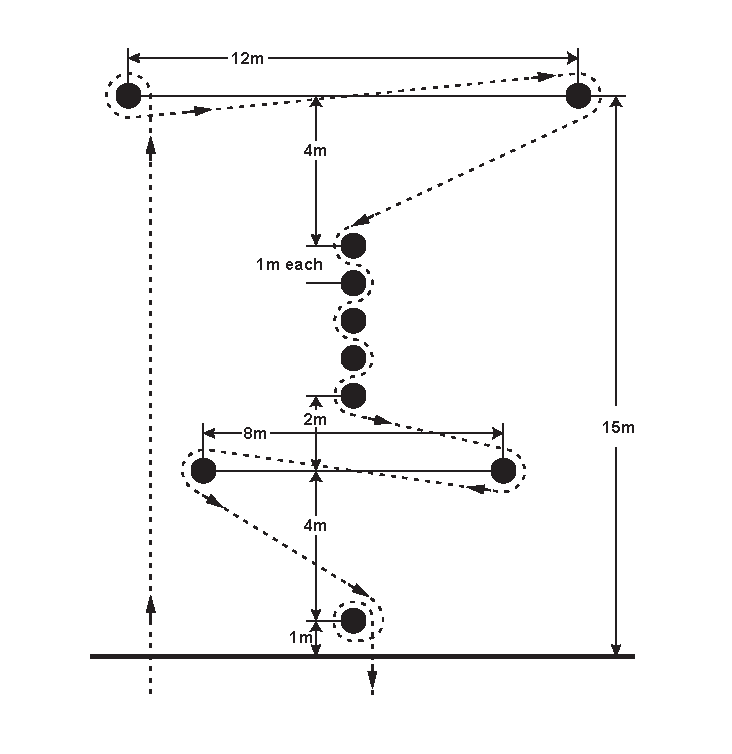
\includegraphics{iuf_slalom}
\end{center}
\vspace{-20pt}
\caption{IUF Slalom Course \label{fig:iuf_slalom}}
\vspace{-10pt}
\end{figure}
Pictured here is the IUF Slalom, in which you must ride around 10 cones in the correct pattern.
Arrows marked on the ground should indicate the direction of the turns for riders unfamiliar with the course.
The rider has to start directly behind the Start line.
The Starter gives the opening, and then the competitor has to start during the next 3 seconds.
The timer is started when any defined point of the tire (for example the part that crosses a low light beam) crosses the start line, and stops when a similar point of the tire crosses the finish line.
If the rider has not yet started after 3 seconds, the timer will start counting anyway.
The rider is not disqualified for this.
Time measurement at start and finish line must be identical to insure accurate time measurement.
It must be secured that riders do not gain momentum before crossing the start line (no flying starts).
Remounting is not allowed. 
Cones may be hit, but not knocked over.
The course must be followed correctly, including the direction of turns.
The last cone must be completely circled before the rider's time is taken at the finish line.
Riders who go the wrong way around a cone can go back and make the turn the correct way with the clock still running.
The cones used are plastic traffic cones.
For official competition, cones must be between 45 and 60 cm tall, with bases no more than 30 cm square.
The course must be set up accurately.
The proper positions of the cones should be marked on the ground for a cone to be replaced quickly after it has been knocked over.
Riders get two attempts.

\section{Alternate, Optional or Fun Events \label{sec:track-field_alternate-optional-fun-events}}
These are optional events, not guaranteed to be included in every unicycle convention.
They can be held with as much, or as little, level of formality and importance the host chooses.
Age group breakdown is also up to the host.
All of the events in this section have been run before, using these rules.
If a large convention advertises events with the names of the ones detailed in this section, they must use the rules provided here.
If hosts desire to do variations on these rules, the events must be labeled accordingly.
Example: ``Track Gliding; Modified''.
In cases such as this, hosts must remember to provide detailed rules for these events at the same time the events are announced.

\subsection{Relay (Track)}
Usually 4 x 100m or 4 x 400m like in athletics.

The takeover zones are 20 meters long and must be marked on the track.
Riders may remount if necessary, and must pick up the baton if it is dropped.
The handover of the baton must be within the takeover zone.
This means that before the baton crosses the start mark of the takeover zone \emph{only} the incoming rider is in touch with the baton and at the end of the takeover zone \emph{only} the outgoing rider is in touch with the baton.
Riders may not throw the baton to make a pass and may not touch the ground with any part of their body while making a pass.
If the baton is not handed over within the marked takeover zone, the team will be disqualified.
Leaving of the lane within the takeover zone or when remounting does not result in disqualification as long as the riders do not obstruct, impede or interfere with another rider's progress.
There is no defined preparation area for the next riders as long as they stay within their lanes.

Mixed male/female teams may be used, and reasonable age groups may be used depending on the number of expected competitors of the event.
Each relay team may have any mix of ages, the age of the oldest rider determines the age group.

\subsection{Coasting Events \label{sec:track-field_coasting-events}}
An event to determine which rider coasts the furthest distance.
Riders' coasting distances are measured from a `starting line' with a 5 meter minimum, which will be marked by a `qualifying line.'
If the rider does not cross the qualifying line it will count as a failed attempt.
The farthest distance from the line wins.
The distance is measured to the rearmost part of the rider that touches the ground when dismounting, or to the rear of the tire where the rider stops coasting.
Remounting is not allowed.
Riders must not touch any part of their tires, wheels or pedals while coasting.
Riders get two attempts.
If a rider crosses the coasting line (front of the tire) not in coasting position, he or she is disqualified in that attempt.
The riding surface should be as smooth and clean as possible, and it may be straight or curved.
Ample time must be allowed for all competitors to make some practice runs on the course before the official start.
The type of event(s) to be used should be announced well in advance of the competition.
Crank arm rules do not apply in any coasting or gliding events.

\subsubsection{Road Coasting}
This event is best held on a roadway with a very slight downward slope.
Riders are allowed an unlimited distance to speed up and start coasting before the starting line.

\subsubsection{Track Coasting \label{subsubsec:track-field_alternate-optional-fun-events_coasting_track-coasting}}
30 meter speed-up distance.
This event is held only on a track, or a very level, smooth surface.
Wind must be at a minimum for records to be set and broken.
This event can be compared with other races at different tracks worldwide.

\subsubsection{Downhill Coasting}
This is a speed coasting event.
Riders start from a standstill, or speed up to the `starting line'.
Riders are timed over a measured distance to the finish line.
Dismounts before the finish line disqualify the rider in that attempt.
The slope must be very gradual for this event to be safe, and helmets are mandatory.

\subsubsection{Indoor Coasting}
30 meter starting distance.
This event is held indoors in a gym, or on a very level, smooth surface.
Rider will coast in a circle on the outer edge of the gym, separated by cones.
Both directions are allowed for the start (clockwise or counterclockwise), and rider will have a maximum of 30m before beginning to coast.
Indoor coasting is the recommended coasting competition at a Unicon.

\subsection{Gliding Events \label{sec:track-field_gliding-events}}
Gliding is like coasting, but with one or both feet dragging on top of the tire to provide balance from the braking action.
These events are similar to the coasting events above, with riders gliding for time or distance from a given point.
The rules are the same as for the coasting events (above) with the addition that the riding surface must be dry.
Coasting is allowed.

\subsubsection{Slope Glide Or Track Glide}
A slope glide can be done on a small hill.
Riders start on the hill, gliding down to level ground and continuing as far as they can before stopping.
This event can have a limited starting distance, or no starting distance at all, with riders gliding from a dead stop.
If it is a Track Glide, it is held on a track with the same rules as Track Coasting (see section \ref{subsubsec:track-field_alternate-optional-fun-events_coasting_track-coasting}).

\subsubsection{Downhill Glide}
A downhill race for speed.
Riders start from a standstill, or speed up to the `starting line.'
Riders are timed over a measured distance to the finish line.
Dismounts before the finish line disqualify the rider in that attempt.
Helmets are mandatory.

\subsection{Slow Forward}
In Slow Forward, the rider riders in a continuous forward motion as slowly as possible without stopping, going backward, hopping or twisting more than 45 degrees to either side on a 10 m x 15 cm board. There are no crank arm length or wheel size restrictions for this event. 

Riders must wear shoes. No other safety gear is required.

\subsubsection{Timing}
The position of the unicycle during a Slow Race is measured from the bottom of the unicycle wheel.
In a Slow Race, the rider starts behind the starting line. On command by the starter, the rider has 10 seconds to start forward motion and let go off the starting post.
The timer starts recording time when the bottom of the wheel crosses the starting line.
The time stops when the bottom of the wheel crosses the finish line, or touches the ground after the end of the board that marks the finish line. 


\subsubsection{Penalty Rules}
The judges give penalties to riders who seem to make ``micro-errors'' (for example twisting about 46 or 48 degrees or vibrations of the wheel) or if they are in doubt if an error was made. Each penalty deducts one second from the ridden time.
Riders are still disqualified if their wheel comes off the board or other obvious errors are made, for example dismounting or twisting 90 degrees.

\subsubsection{Rules For International and Large Competitions}
These rules are required to be used at Unicon.

\textbf{Qualification round:}
\begin{itemize}
\item Riders must complete a time equal or greater than 45 seconds to move on to the finals.
\item Riders get two attempts to complete this result.
\item Previous results are valid: If a rider has already completed a result of 45 seconds or greater at another competition, they can start automatically in the finals and they don't have to take part in the qualification round, provided that the result can be found in an official result list.
\item The boards can be marked with tape on the floor.
\item No age groups will be ranked. 
\item Results will not be valid for records (world, continental, national and regional records).
\end{itemize}

\textbf{Final round:}
\begin{itemize}
\item There will only be one team of judges, in order to have a fair competition. 
\item All riders who are qualified for the final round start here.
\item Riders get two attempts.
\item Only results from the finals will be valid for records ( world, continental, national and regional records).
\item The champion is the rider who performs the best result in the final round.
\end{itemize}

\subsubsection{Options for Smaller Competitions}
At regional or national championships, the host can decide to offer age groups ranking and awards, and adjust the qualification time to a lower time as needed.
If the hosts decides to offer age groups, the results from the qualification round count for age group results.
However, the final round is still required.
The results from the final round will also be included in the ranking for age group results.
Previous results from other events are not valid to be included in the age group results.
If the host decides to offer age groups, the board size of 10 m x 30 cm can be used for the 0-10 age group.

\subsection{Slow Backward}
This is the same as the Slow Forward race, with the following differences:
\begin{itemize}
\item Riders ride backward.
\item It is an error to ride forward.
\item Riders ride on a 10 m x 30 cm board.
\item If the host of a national or regional championship decides to offer age groups, the board size of 10 m x 60 cm can be used for the 0-10 age group.
\item Riders move on to the finals if they have completed a time equal or greater than 40 seconds, previous results are valid.
\end{itemize}


\subsection{Stillstand}
Stillstand is a competition in which the rider attempts to balance as long as possible.
The rider cannot hop or turn the tire more than 45 degrees, and must remain on a 25 cm long, 10 cm wide, and 3 cm tall block of wood.
The competition should take place indoors on a level surface
The only required safety gear is shoes.

Each participant has 2 attempts that can be done at any time during the time window set by the host.
The host can decide to add to each of the 2 attempts a window up to 20 seconds, in which the competitor can start the number of tries needed.

The starting post is placed anywhere the participant prefers.
Time starts running when the competitor lets go of the starting post.
After time starts running, the starting post will be taken away.
Time stops at the moment when the participant rides off the board, dismounts, starts hopping or turns the tire more than 45 degrees.

There are no finals for the Stillstand competition.
The overall results will be determined by the best results per gender.

\subsection{700c Racing}
Races of any length and type can also be conducted in a 700c wheel category.
\begin{itemize}
\item Maximum bead seat diameter (BSD): 622 mm.
\item If these races are intended to exclude 24$"$ wheels, sizes must be greater than 618 mm.
\item No restrictions on crank length.
\item Beyond these, 700c unicycles must comply with all other requirements for racing unicycles.
\item The host may choose age groups.
\end{itemize}

\subsection{Unlimited Track Racing}
An unlimited race is one in which there are no unicycle size restrictions.
Any size wheels, any length crank arms, giraffes or any types of unicycles (see definition in chapter \ref{chap:general_definitions}) are allowed.
All other Track racing rules apply.

\subsection{Juggling Unicycle Race}
The traditional distance is 50 meters.
Riders use the 5m line from the One-Foot Race, and must be juggling when they cross this line.
Three or more non-bouncing objects must be used.
If an object is dropped (hits the ground) or the juggling pattern is otherwise stopped, the rider is disqualified.
Two balls stopping in one hand during a 3-ball cascade is defined as stopping.
Riders who start by juggling four or more objects may drop one, as long as their pattern continues, unbroken, into three.
The juggling pattern must be `in control' when the rider crosses the finish line.
`Control' is determined by the Referee.

\subsection{Ultimate Wheel Race}
An ultimate wheel is a unicycle with no frame or seat.
The traditional distance is 10m for 0-10 riders, and 30m for 11-UP riders.
Maximum wheel size is 618 mm (24$"$) for all ages, with 125 mm minimum crank arm length or 250 mm between pedal holes.
The host may allow other limitations, or none, if these details are announced well in advance.

\subsection{50m Fast Backward}
Riders must face and pedal backward.
The Starter lines up the rear of the tire above the start line.
Helmets are mandatory.
Timing is stopped when the rear of the tire crosses the finish line.

\subsection{Medley}
This is a race involving riding several different ways of riding.

\textbf{Example:} Forward 25m, seat in front 25m, one foot 25m, hopping 10m, with 5m transition areas.
Rules are set by the host.
Remounting is allowed.

\subsection{Slow Giraffe Race}
This is the same as slow forward, but on giraffes.
Helping hands can be used as starting posts.
No limits on size or gear ratio, but unicycles must have their pedal axle above the wheel axle, with a chain, belt, or other form of drive system.
\part{Jumps \label{part:jumps}}
\parttoc

\singlechapter{Jumps \label{chap:Jumps}}

Unicycling versions of the High Jump and Long Jump.

\section{Unicycles}
Standard unicycles must be used (see definition in chapter \ref{chap:general_definitions}).
No restriction on wheel or crank size.
Metal pedals are allowed for their strength and better grip.
This may make it impossible to hold this event on a sensitive track surface.

\subsection{Broken Unicycle}
If the unicycle breaks during an attempt, a new attempt must be given to the rider.

\section{Practice Areas}
The organizer should provide a place and equipment similar to those used for the official competition so the riders can practice before making their official attempts.
The equipment should be available during the whole length of the event, and even before if the organizer decides so.

For bigger events such as Unicon, national or continental events, the organizer must provide said equipment.

\section{Safety Gear}
Riders must wear shoes, kneepads, gloves and a helmet (definitions in chapter \ref{chap:general_definitions}).

\section{High Jump}
The rider and unicycle jump over a bar, without knocking it down, and ride away without a dismount.
There are three parts to a successful jump: 
\begin{enumerate}
\item Riders must mount before the start line, to show they are on the unicycle and in control.
The attempt starts when the rider crosses the start line.
The rider may break off from a jumping attempt before leaving the ground, but must then start again from behind the start line.
That attempt then doesn't count.
\item Riders must jump over the bar without knocking the bar off the apparatus.
The bar can be hit as long as it does not fall.
If the bar falls before the rider crosses the finish line, it counts as an unsuccessful attempt.
\item After landing, the rider must stay in control of the unicycle until he cross the finish line without dismounting, touching a hand to the ground or any other object, or knocking down the bar or any of the high jump apparatus.
Riders get two attempts at each height.
The rider starts at a low height and after each successful attempt, the height increases at set intervals until the rider fails to be successful on both attempts.
When the rider fails both attempts, the maximum height that was completed is recorded.
\end{enumerate}

\subsection{Setup}
Around the High Jump apparatus a circle with a radius of 3 meters must be marked.
This circle is start and finish line.
The rider can cross it wherever he wants.
Riders must ride or hop across the finish line for the attempt to count.
Successfully crossing the finish line is judged the same as in racing (see section \ref{sec:track-field_finishes}).
The bar must be held loosely in the jumping apparatus so it can fall or break away if the rider does not complete the desired height.
Magnetic systems are not allowed.
The bar shall have a minimum diameter of 2cm.

\section{Long Jump}
The rider jumps as far as possible from a jump marker, to a landing without a dismount.
The rider must then continue riding across a finish line to show control.
Riders must clear 3 markers (jump marker, landing marker and finish line) to make the jump count.
Riders may jump with the wheel going forward or sideways.
After landing, the rider must stay in control of the unicycle for the remainder of the distance from the jump marker to the finish line without dismounting, or touching a hand to the ground or any other object.
If the tire touches the jump marker before takeoff or the landing marker, it counts as a foul.
Riders may break off in a run as long as he is between start line and jump marker but if they cross or touch the jump marker, the attempt counts, including fouls.
Riders get two attempts for each length.
The farthest non-fouling, successful jump is recorded.

To avoid endless competitions, the length to jump will always increase by 5cm for each round.
Once there are only 5 riders left, it's up to the riders to decide in which steps they continue.
For each age group the minimum length should be adjusted to a useful level such as 150cm for 15+ and 70cm for 0-15.
The host can adjust this depending on the level at his competition.

\subsection{Setup}
The riding area consists of a start line, a jump marker, a landing marker and a finish line beyond the jump marker.

The finishing line should be at least 4 meters from the landing marker but no more than 8 meters away.
We suggest that judges set up the finishing line 8 meters from the jump marker and move it further away if need during longer jumps.
Riders must ride or hop across the finish line for the attempt to count.
Successfully crossing the finish line is judged the same as in racing (see section \ref{sec:track-field_finishes}).
The start line must be a minimum of 25 meters in front of the jump marker to allow the riders to accelerate.
There must be an area behind the finishing line which is a minimum of 7 meters long and 2 meters wide as safety zone.
Riders may use all or part of the 25 meters between start line and jump marker.
Riders are also allowed to start from beside to be able to do accelerated side jumps.
Markers for takeoff and landing (jump marker and landing marker) must consist of a material which not can be deformed to have the same conditions for all riders.
The markers must be at least 1.20 meter in width (across the runway), no more than 10 mm in height (above the runway), and no less than 5 centimeters in depth (front to back).
A Long Jump competition needs a minimum area of 40x2.5 meters.

\subsection{Judging}
The rider must clear the jump marker and the landing marker without touching them; he also has to clear the finish line to make it a valid jump.
Jump distance is measured between the outer edges of the jump and landing marker.
There has to be at least one judge (better two) to look at the markers.
For national championships and Unicons, two judges are always needed; one to observe each marker.

\part{Road Racing \label{part:road_racing}}
\parttoc
\addstarredchapter{Road Racing}
\singlechapter{Road Racing \label{chap:road_racing}}

\section{Definition} %more needed here?
These are races held usually on roadways or bike paths, generally for longer distances than our events on the track.
All riders may race together and be separated by age group afterward.

\section{General Rules}
Water/food stations are recommended.
Personal music systems are not allowed for any races on public roads where there may be motorized traffic.
Riders can be divided by age and/or unicycle type, such as 24$"$ and 29$"$ track unicycles, Standard (any size wheel and cranks), and Unlimited (see definition in chapter \ref{chap:general_definitions}).
24$"$ and smaller wheels are not allowed for races longer than 20km without express permission of the racing director.

\subsection{Ungeared Awards}
If there are 5 or more geared riders in an Unlimited event, the fastest 3 ungeared riders from both the male and female categories will be awarded with an ungeared title for that event.
This is only for the overall classification, not for Age Groups.

\section{Safety Gear}
Riders must wear shoes, kneepads, gloves and a helmet (see definition in chapter \ref{chap:general_definitions}).
The Referee has final say on whether a rider’s safety equipment is sufficient.
Elbow pads are also good considerations for safe unicycle racing.
The Starter will remove from the starting line-up any riders not properly equipped to race, including riders with dangerously loose shoelaces.

\section{Age Groups}
The following age groups are the minimum required by the IUF to be offered at the time of registration for any Road Racing discipline: 0-13, 14-18, 19-29, 30-UP.
For any discipline for which there is a Standard 24$"$ wheelsize category, also an age group 0-10 (20$"$) must be offered.

Convention hosts are free to offer more age groups, and often do.
For example, a full range of offered age groups might look like 0-8 (20$"$), 9- 10 (20$"$), 0-12, 13-14, 15-16, 17-18, 19-29, 30-39, 40-49, 50-59, 60-UP.
All age groups must be offered as male and female age group.

\section{Race Distances and Distance Measurement}
Traditional road race distances have been: 
\begin{itemize}
\item 10k with Unlimited and Standard 24$"$ classes, and 
\item Full Marathon (42.195k) with Unlimited and possibly Standard 29$"$ classes.
\end{itemize}
However, any distances or wheelsize classes can be used for Road Races.

\subsection {Distance Measurement for Traditional Distances}
In the case where a traditional race distance is used (such as 10k or Marathon---42.195k), the course must be accurately measured along the shortest possible path.
The course must be guaranteed to be no shorter than the advertised distance.

The following procedure is acceptable for accuracy.
A more accurate method is of course allowed.
\begin{enumerate}
\item Set out a calibration course on straight, flat asphalt, with a minimum length of 100 meters, using a steel measuring tape of 5 meters or longer.
\item Ride the calibration course at least once with a bike or unicycle (minimum wheelsize 24$"$).
Ride normally, without too much wobble, and at normal speed.
Take care that mounting and dismounting don't cause the wheel to swerve, or be lifted from the surface.
Carefully count the number of wheel revolutions required to ride the calibration course.
Include partial wheel revolutions (for example through counting the number of spokes passed for the last partial revolution).
\item Calculate the wheel rollout (meters per revolution) from step 2.
\item If you are going to use a cycle computer: enter the wheel rollout value to the nearest millimeter in a reliable cycle computer with a wheel sensor (such as a magnet).
\item Fit the cycle computer, or a wheel revolution counter, to the same bike or unicycle used in Step 2.
\item Ride the actual race course, following the shortest possible path.
Take care to ride in the same way as in step 2.
\item Read the distance from the cycle computer, or calculate from wheel revolutions and wheel rollout.
\item Calculate the applicable safety margin by adding up (1) $0.4\%$ of the measured distance, and (2) the resolution of the cycle computer distance readout.
\textbf{Example:} if your cycle computer shows $10.15\unit{km}$, the safety margin is $0.4\% \cdot 10.15\unit{km} + 0.01\unit{km} = 0.0506\unit{km} = 50.6\unit{m}$.
\textbf{Note:} you can skip (2) if you use a wheel revolution counter that can resolve single wheel revolutions.
\item Add the safety margin to the actual course (for example shift the start and/or finish line), to guarantee that the course is at least the advertised distance.
\end{enumerate}
Note that Steps 2 through 7 must be done without breaks.
The same rider should ride the calibration course and the race course.
The tire pressure should not be altered in the mean time.

\subsection {Distance Measurement for Other Distances}
In the case where a non-traditional race distance is used (such as any distance other than 10k or 42.195k), the course must be measured with an accuracy of plus or minus 3\% or better.
\textbf{Example:} if a race is advertised as 100 km, the actual distance must be between 97 and 103 km.
A good consumer-type GPS unit is acceptible, provided the track shows continuous reception of suffucient satellites (no `stray' data points, or missing points).
Also acceptable is the Distance Measurement Tool of Google Maps.
A car odometer, on the other hand, might easily be off by more than 3\%, and is therefore not acceptable unless you know how to correct it.
Obviously, using a more accurate measurement is allowed, such as the method described for `traditional distances'’'.

\section{Unicycles for Racing}
Only standard unicycles may be used.
Riders may use different unicycles for different racing events, as long as all comply with the rules for events in which they are entered.
\subsection{Wheel Size and Crank Arm Limit}
\begin{itemize}
\item For a ``Standard 29$"$ Unicycle'' the outside diameter of the tire may not be larger than 768mm and there is no minimum crank arm limit.
No gearing may be used.
\item For a ``Standard 24$"$ Unicycle'' the outside diameter of the tire may not be larger than 618mm and crank arms may be no shorter than 125mm.
No gearing may be used.
\item For a ``Standard 20$"$ Unicycle'' the outside diameter of the tire may not be larger than 518mm and crank arms may be no shorter than 100mm.
No gearing may be used.
\end{itemize}

\section{Heat Assignments}
Line-up order and heats must be assigned prior to the race.
There are three allowable formats for designating the starting configuration of a Road Race: individual start (section \ref{subsec:road_heat-assignment_individual-start}), heat start (section \ref{subsec:road_heat-assignment_heat-start}), or mass start (section \ref{subsec:road_heat-assignment_mass-start}).

To determine which start configuration to use, read the following rules from top to bottom.
Once you have an outcome, \textit{disregard} the remaining rules.
\begin{itemize}
\item If this is an ``Individual Time Trial'' format race, use individual start.
\item If the course is too narrow to allow for racers to safely and fairly start in heats, use individual start.
\item If you cannot safely start five or more riders across, use individual start.
\item If the starting field consists of 30 riders or less, use a mass start.
\item If the course does not allow for ten riders to ride abreast for at least 500m before the course narrows, use heats of 12 or more riders.
\item If the starting field consists of more than 50 riders, use heats of 20 or more riders.
\item In all other cases, use a mass start.
\end{itemize}
Standard racers should always start separately from Unlimited racers, also in the case of a mass start or heat starts.
Unlimited racers should start first, unless there is no risk that Unlimited riders have to pass standard riders (for example they race on different days).

In the sections below, ``fastest rider'' means ``fastest rider by seed time.'' Seed time is defined as an estimated finish time, preferably based on past performance in similar event(s).
If no seed time is submitted by the rider or their coach, the organisation can assign a seed time.

\subsection{Starting Order}
The goal in determining the starting order is to sort racers fairly by speed while still making sure that genders race amongst themselves.
Unless otherwise noted below, the fastest riders start first, and also within a start group (heat or mass start), riders should be positioned in the line-up by speed with the fastest in front.
Starting order can be determined by seed time, or from the results of a previous Road Race in that competition.
For example, if the Marathon follows the 10k, the results of the 10k can be used to determine the starting order for the Marathon.
In the case that a racer does not have a seed time, and is signed up for a particular event (such as the Marathon) and did not participate in the previous race (such as the 10k), the Racing Clerk has the right to assign a starting position where they see fit.

\subsection{Individual Start \label{subsec:road_heat-assignment_individual-start}}
Each rider is individually started at a fixed time interval, such as every 20 or 30 seconds.
Riders are sorted by speed with the fastest rider going first.
(Except in the case of an Individual Time Trial, where the race can start with either the fastest or slowest rider.)

\subsection{Heat Start \label{subsec:road_heat-assignment_heat-start}}
Heats should consist of at least 12 riders, either male or female (no mixed heats).
Heats are sorted by speed with the fastest heat going first.
Heats should be started every one to five minutes.

\textbf{The following example describes how this can be done:}
The first three heats might contain the fastest men, then a heat of the fastest women who are of proportionate speed with the third heat of men.
This format makes sure that the top women start together while still giving them the opportunity to race and pace off of men of similar speed.

\subsection{Mass Start \label{subsec:road_heat-assignment_mass-start}}
A mass start is a start in which all racers of a certain class (such as Standard or Unlimited) start together.
Genders start at the same time.

\section{Special Marathon Events}
Exceptions from the default rules may be allowed for a marathon race that is embedded in a big city marathon (such as Düsseldorf Marathon).
This allows the unicycling organizer to follow some requirements of the main marathon organizer in order for the unicycling marathon to fit within the larger event.

The following exceptions to the rules may be made:
\begin{itemize}
\item Mass start / Group start (Mass start could be forced by the main host for schedule requirements) 
\item Start groups do not have to be per gender and/or wheel size
\item Netto times (time from when the rider's wheel crosses the start line) can be used for placements while the Brutto time (time from when the race is started) counts for Records.
\end{itemize}

\section{Starting}
Riders start mounted, holding onto a starting post or other support.
The Starter will give a four-count start.
For example: ``One, two, three, BANG!''
There should be about 3/4 second between each element in the count, with the same amount of time between each of them.
This allows riders to predict the timing of the gun, for a fair start.
Starters should practice this before the races begin.
Timing of the count is very important for an accurate start.
This count can be in the local language, or a language agreed upon before competition starts.

As an alternative a Startbeep apparatus can be used.
In that case we have a six-count start.
For example: ``beep - beep - beep - beep - beep - buup!''
The inter-beep timing is one second.
The first 5 beeps have all the same frequency.
The final tone (buup) has a higher frequency, so that the racer can easily distinguish this tone from the rest.

Riders start with the fronts of their tires (forward most part of wheel) behind the edge of the starting line that is farthest from the finish line.
Rolling starts are not permitted in any race.
However, riders may start from behind the starting line if they wish, provided all other starting rules are followed.
Riders may lean before the gun fires, but their wheels may not move forward before the gun fires.
Rolling back is allowed, but nothing forward.
Riders may place starting posts in the location most comfortable for them, as long as it doesn't interfere with other riders.

A rider’s starting time is taken as when their heat begins (when the gun goes off) regardless of when they actually cross the starting line.
\subsection{Riders Must Be Ready}
Riders must be ready when called for their races.
Riders not at the start line when their race begins may lose their chance to participate.
The Starter will decide when to stop waiting, remembering to consider language barriers, and the fact that some riders may be slow because they are helping run the convention.

\section{False Starts}
A false start occurs if a rider's wheel moves forward before the start signal, or if one or more riders are forced to dismount due to interference from another rider or other source.

There are several options on how to deal with false starts:
\begin{itemize}
\item \textbf{One False Start Allowed Per Rider:}
In case of a false start, the heat is restarted.
Any rider(s) who caused their personal first false start may start again.
Any rider(s) causing their personal second false start are disqualified.
\item \textbf{One False Start Allowed Per Heat:} 
In case of a false start, the heat is restarted.
For the first false start of a particular heat, all riders may start again.
Thereafter, any rider(s) causing a false start are disqualified.
\item \textbf{Time Penalty:}
In case of a false start, the heat is not restarted.
If a false start occurs by one or multiple riders, these riders receive a time penalty (such as 10 seconds).
\end{itemize}
If a heat has to be restarted, the Starter will immediately recall the riders, for example by firing a gun or blowing a whistle or any other clear and pre-defined signal.

If the race is started using individual starts or heat starts (see sections \ref{subsec:road_heat-assignment_individual-start} and \ref{subsec:road_heat-assignment_heat-start}) a time penalty is the recommended option.
In the case of a mass start (section \ref{subsec:road_heat-assignment_mass-start}), any option is viable.
The host must announce the false start method at least two months before the event.

\section{Riding Behavior}

\subsection{Passing}
An overtaking rider must pass on the outside, unless there is enough room to safely pass on the inside.
Riders passing on the inside are responsible for any fouls that may take place as a result.
No physical contact between riders is allowed.
The slower rider must maintain a reasonably straight course, and not interfere with the faster rider.

\subsection{Dismounts}
In Road Racing, dismounting and remounting is allowed. 
If a rider is forced to dismount due to a fall by the rider immediately in front, it is considered part of the race and both riders must remount and continue.
The Referee can override this rule if intentional interference is observed.

\subsection{Illegal Riding}
This includes intentionally interfering in any way with another rider, deliberately crossing in front of another rider to prevent him or her from moving on, deliberately blocking another rider from passing, or distracting another rider with the intention of causing a dismount.
A rider who is forced to dismount due to interference by another rider may file a protest immediately at the end of the race.
Riders who intentionally interfere with other riders may receive from the Referee a warning, a loss of placement (given the next lower finishing place), disqualification from that race/event, or suspension from all races.

\section{Finishes}
Finish times are determined when the front of the tire first crosses the vertical plane of the nearer edge of the finish line.

Riders are always timed by their wheels, not by outstretched bodies.
If riders do not cross the line in control, they are awarded a 5 second penalty to their time.
``Control'' is defined by the rearmost part of the wheel crossing completely over the vertical finish plane (as defined above) with the rider having both feet on the pedals.
(Note: a rider is not considered in control if the unicycle crosses the finish line independent of the rider.
The finish time is still measured by when the wheel crosses the vertical finish plane and the 5 second penalty is applied.)

In the case where a rider is finishing with a broken unicycle, the rider must bring at minimum the wheel to the finish line, and time is still taken when the wheel crosses the finish line.
The 5 second penalty is applied.

If finish times for a race are timed using microchips or other non-photographic electronic equipment, finish order must be verified by photo timing equipment if the finishers are within 0.1 seconds of each other.
Also, in the case where a world record is suspected of being set, the time must be verified with photo timing equipment.

\section{Optional Race-End Cut-Off Time}
It may be necessary to have a maximum time limit for long races, to keep events on schedule.
When this is planned in advance, it must be advertised as early as possible, so attending riders will know of the limit.
Additionally, at the discretion of the Racing Director, a race cut-off time may be set on the day of or during an event.
The purpose of this is to allow things to move on if all but a few slow racers are still on the course.
These cut-offs need not be announced in advance.
At the cut-off time, any racers who have not finished will be listed as incomplete (no time recorded, or same cut-off time recorded for all).
Optionally, if there is no more than one person on the course per age category and awards are at stake, they can be given the following place in the finishing order.
But if each participating age category has had finishers for all available awards (no awards at stake), there is no need to wait.





\part{Mountain Unicycling \label{part:muni}}
\parttoc
\addstarredchapter{Mountain Unicycling}
\chapter*{Mountain Unicycling \label{chap:muni}}

\section{Definition}
For purposes of these rules, mountain unicycling (muni) refers to off road races over any type of terrain.
Races can vary from a single heat race with all riders starting together, to a time trial type of arrangement with riders going individually, at intervals.
Mountains are not required.
Terrain can be anything from dirt to paved areas, hills, ditches, curbs, rocks, sand, mud, or grass.
Unless otherwise noted, there are no restrictions on wheel size, crank arm length, brakes or gearing.

\section{Disciplines}
Mountain Unicycling competitons usually involve Uphill (section \ref{sec:muni_uphill}), Downhill (section \ref{sec:muni_downhill}), and Cross Country (section \ref{sec:muni_xc}), but other events such as North Shore (a technical compotition) and Slopestyle (a trick/style competition) can be included.
If the hosts wish to include events other than the first three (Up, DH, XC), they must remember to provide detailed rules for these events at the same time the events are announced.

\section{Safety Gear}
For all muni events, riders must wear shoes, kneepads, gloves/wristguards and helmets (see definition in section \ref{sec:general_definitions}).
The IUF allows no exceptions to this for muni events.
Additional equipment such as shin, elbow or ankle protection are optional.

\section{Muni Courses}
Courses must be clearly marked, so that riders can easily see where to go.
Very dangerous sections should be secured (e.g. by removing sharp stones/branches from areas where riders are likely to fall/run into due to the physics of the course).
Unless otherwise noted, non-lane passing rules apply (see section \ref{subsec:track-field_lane-use_non-lane-races}).
All courses should strive for a balance of speed, excitement, and safety.

For all muni races, every rider must get the chance of at least one test run to get familiar with the track before the actual race.
If possible, the track should be open for training during all days of the event prior to the race.
For multiday events the muni competitions should take place during the second half of the event in order to give riders more time to practice on the course.

\section{Starting Modes}
The fastest riders should always start first, regardless of the starting mode.
The order can be determined by seeding runs.
There are three different types of starting modes, that can be used in muni races.
\begin{enumerate}
\item \textbf{Mass starts:} All riders start at the same time.
Mass starts must not be used when the race duration is expected to be shorter than 30 minutes.
The track must provide sufficient space for passing in the first section, so that the field of starters is aligned before the track narrows down.
Space for passing must be given along the track.
Mass starts with more than 40 riders have to be split to avoid accidents.
\item \textbf{Heat starts:} Groups of riders start at intervals that can vary from 30 seconds to a few minutes.
The maximum number of riders per heat is determined by the average width of the first 100m of the track.
There can be one rider for each meter in width.
\item \textbf{Individual starts:} Individual riders start at intervals that can vary from 30 seconds to a few minutes.
\end{enumerate}

\section{Age Groups}
Age groups must be offered as male and female age group.
There must not be any age group specific restrictions on equipment.
The following age groups are the maximum allowable for muni competitions:

\begin{tabular}{ l l}
Under 15 & Youth \\
15-16 & Juniors \\
17-18 & Rookies \\
19-29 & Elites \\
30-49 & Masters \\
50+ & Veterans \\
\end{tabular}

\section{IUF Muni Results}
The host must publish two lists of results for each discipline after the competition: Age group based ranking and overall ranking (separating
male/female).

\section{Dismounts and Dismounted Riders}
Dismounts are allowed in all muni races unless otherwise noted.
In mass-start events, dismounted riders must yield to mounted riders behind them as quickly as possible after a dismount, and until re-mounted.
Riders may not impede the progress of mounted riders when trying to mount.
If necessary they must move to a different location so mounted riders can pass.
If riders choose not to ride difficult sections of the course, they must not pass any mounted riders while walking or running through them.
In time trial-type events, see below for variations based on the other event details.
Violations of these non-riding rules may result in disqualification or a time penalty, to be determined and announced before the race start.
Riders must also ride completely across the finish line, as described in section \ref{sec:track-field_finishes}.

\section{Uphill Race \label{sec:muni_uphill}}
An Uphill muni race challenges riders' ability to climb.
Courses may be short and steep or longer, endurance-related challenges.
Generally it is a timed event, but on an extremely difficult course, riders can be measured as to how far they ride before dismounting.
The race can be offered as a no-dismounts challenge, which either measures who gets the farthest, or disqualifies anyone who doesn't complete the distance without a dismount.
Multiple tries can be allowed, or the race can be a simple timed event.

\subsection{Dismounted Riders}
If the Uphill race is run as a time trial, riders are intended to ride the entire distance.
In the event of a dismount, the rider must remount the unicycle:
\begin{enumerate}[(a)]
\item At the point where the dismount occurred if the unicycle falls back down the course toward the start.
\item Where the unicycle and/or rider come to a stop after dismounting.
Excessive running/walking/stumbling after a dismount may be grounds for a
penalty at the discretion of the Referee.
\item Riders may also choose to back up (toward the start line) from one of those spots to remount, if they prefer the terrain there.
\end{enumerate}

\section{Downhill Race \label{sec:muni_downhill}}
A Downhill muni race is a test of speed and ability to handle terrain.
Courses must be primarily downhill but may include flat or uphill sections.
Recommended course length is 2.5 km, or 1 km at a minimum, depending on available terrain, trails and schedule time.
For a course length less than 2 km, two separate runs should be held.
In this case the ranking of the riders is based on the fastest of the two runs.
Riders should race one at a time, released at regular time intervals.
If the schedule has a small time window for the race, riders should be run in heat sizes that allow passing on the course, and do not bottleneck at the beginning.

\subsection{Dismounted Riders}
Dismounted riders must not impede the progress of, or pass mounted riders.
They must remain aware of riders coming from behind, and not block them with their
unicycles or bodies.
Running is not allowed, except momentarily to slow down after a dismount.
Riders may walk if necessary.
Riders may receive a time penalty or be disqualified if they disregard this rule.

\section{Cross Country (XC)\label{sec:muni_xc}}
A Cross Country race should be at least 10 km or longer, depending on available terrain, trails and schedule time.
If only shorter trails are available, riders can be required to complete two or more laps of the course.
It is basically any muni race that is not specifically focused on downhill or uphill.
The course can contain any amount of uphill or downhill riding and is to be about fitness, and ability to ride fast on rough terrain.

\subsection{Dismounted Riders}
If the event is held as a time trial, dismounted rider restrictions must be announced before the start of the race.
Depending on course length and difficulty, dismounted riders may be required to walk, or walk only limited distance, or have no restrictions at all.



\part{Freestyle and Standard Skill \label{part:freestyle}}
\parttoc

\chapter{Artistic Freestyle \& Standard Skill \label{chap:freestyle} Overview}

\section{The Difference Between These Events}
In Standard Skill, riders demonstrate pure skill and mastery on a standard unicycle, by performing up to 18 skills they have pre-selected.
Standard Skill judging is based on the point value of the skills and quality of their execution, not the `show.'
In Artistic Freestyle, riders perform to music, with costumes, props and any kinds of unicycles.
Riders are judged not only on skill, but also on how well they entertain and put on a show.
There are Individual, Pair, and Group Freestyle events.

\section{Age Groups and Categories}
Age groups and categories may be different for different types of events.
The minimum allowable age groups and categories are listed for each event.
Convention hosts are free to add more age groups but additional categories can only be added when agreed upon by the Artistic Director, Chief Judge, and Event Host.
Categories may not be added or removed at a Unicon without approval by the IUF Board.
Age group is determined by the rider's age on the first day of the convention.
Junior Expert is open to all riders 0-14.
Expert is open to riders of any age, including 0-14.
Riders must state the category in which they are entering for each Freestyle event in which they participate.

\textbf{Example:} Riders who enter Individual Freestyle as Experts can enter Pairs in another category if they wish.
Riders are divided male/female in Standard Skill and Individual Freestyle, but not in Pairs or Group.

\subsection{Riders Must Be Ready}
Riders who are not ready at their scheduled performance time may or may not be allowed to perform after the last competitor in their age group or category.
The Chief Judge will remember to consider language barriers, and that riders may be engaged in convention work to slow them down.
Except for Standard Skill, a rider may not perform before a different set of judges than those that judged the rest of their age group or category.

\section{Safety Gear}
No safety gear is needed.

\section{Categories for Smaller Competitions}
At competitions where the number of Artistic Freestyle competitors is low, the Event Host may choose to only offer categories and no age groups.
This decision would be made to encourage a competition that is fair and engaging for both spectators and competitors.

\subsection{Categories and Time Limits}
Categories are determined by skill level.
The IUF Skill Levels are used as a guide to determine level of skill.
Skill level testing is not required; these numbers are just used as a point of reference.

For Pairs Freestyle the skill levels of the two riders should be averaged to determine category placement.

\begin{tabular}{|l|c|c|}
\hline
\textbf{Category Name} & \textbf{Level} & \textbf{Time Limit} \\
\hline
Novice & 0-3 & 2 minutes \\
\hline
Intermediate & 4-6 & 3 minutes \\
\hline
Expert & 7-10 & 4 minutes \\
\hline
\end{tabular}
 
\subsection{Choosing Categories}
Riders may enter the competition category they wish according to the approximate skill
level of the skills planned for the routine.
Riders who wish to enter a category that falls outside the guidelines must communicate their choice and reasons to the Chief Judge before the competition.
The Chief Judge will review the choices to assure that riders enter categories that match their skills.

\subsection{Promoting Rider(s) to a Higher Category}
Because these categories are determined based on skill level and not age, it can be difficult to determine the correct category for any given routine.
Therefore, there may be a need to promote routines to a higher category after they have been evaluated.

A routine is allowed to have a maximum of three successfully performed skills that are deemed to be higher than the allowed level for the category.
Skills successfully performed is defined as performing the skill for a reasonable distance without falling, given the choreography of the routine.
When this limit of three is exceeded, the routine is to be promoted to the next most difficult level.
Clearly the skill levels are not an inclusive list of all the skills that may be performed in any given routine.
Therefore, the approximate difficulty level of each skill performed in any routine must be evaluated to determine whether or not the skill is too difficult for the given category.

It is up to the discretion of the Chief Judge as to whether or not a routine is promoted to a higher category.
The Chief Judge should take into account the opinions of the other judges when making this decision.

\section{Performance Set-Up}
Competitors are allowed a maximum of two minutes to set up their unicycles and props in the performing area.
Competitors who take too long risk being disqualified.
An extension of the set-up time can be given only by the Chief Judge and must be requested in advance.
Competitors must show a legitimate need when requesting more time, such as numerous props or complicated special effects.

\section{Interruption Of Judging}
An interruption of judging can result from material damage, injury or sudden illness of a competitor, or interference with a competitor by a person or object.
If this happens, the Chief Judge determines the amount of time left and whether any damage may be the fault of the competitor.
Re-admittance into competition must happen within the regulatory competition time.
If a routine is continued and the competitor was not at fault for the interruption, all devaluations coming forth from the interruption will be withdrawn.

\section{Music \label{sec:freestyle_music}}
In Artistic Freestyle events, music is included in the judging and competitors should use it.
In Standard Skill music is not judged.
But background music will be provided during all Standard Skill routines, or competitors may provide their own.
Competitors may also, at their request, have no music played.
It is recommended to have one or more backup copies of all music in case of loss or damage.
For recordable disks, competitors are also recommended to test their music on multiple players to make sure it will work at competition time.

\subsection{Media Types}
The host is required to have the capability of playing recordable CDs.
Other media types may also be supported, at the host's discretion.
The Artistic Director is responsible for announcing what media types will be supported, and making sure the necessary equipment is provided.

\subsection{Music Preparation}
Competitors must provide their music in a type that is supported, and has been announced by the Artistic Director.
All music must be clearly labeled with the competitor name(s), age group or category, event type (such as Pairs), and if needed, the track number.
Whenever possible, competition music should be the first track on the CD.
The DJ (music operator) is not responsible for any errors resulting from unsupported types or mislabeled tracks.

\subsection{Music Volume}
Volume level is controlled by the DJ, at instructions from the Chief Judge.
The base volume for Freestyle music should be loud enough to sound clear, and be heard by all.
For Standard Skill, volume level should not be loud enough to interfere with judge communication, but otherwise similar to the level for Artistic Freestyle.
Some competitors' music may start with especially loud or quiet sections, and the DJ should be advised of these so volume levels do not get compensated in the wrong direction.
Some competitors may request that their music be played at lower levels.
These requests can be made directly to the DJ.
Requests for higher volumes must be approved by the Chief Judge, who has the option of passing this responsibility to the DJ.

\subsection{Special Music Instructions}
Some competitors may have special music instructions, such as stopping or starting the music at a visual cue, changing volume level during the performance, etc.
The DJ is not responsible for errors carrying out these instructions.
For best results, the competitor should supply a person to coach the DJ during the performance, so there are no mistakes.
If the DJ receives instructions that sound unusual, the Chief Judge should be consulted for approval.

\section{Announcing Of Results}
Final results will be continuously announced and/or posted for public view.
Results Sheets will be posted after each age category of an event.
The protest period begins at this point.

\section{Protests}
Must be filed in writing, within 15 minutes from the posting of event results.
Protest against judges' scores is not permissible.
Protest is only possible against calculation mistakes or other mistakes not connected to the scoring.
The Chief Judge must resolve all protests within 30 minutes from receipt of the written form.

\section{Artistic Freestyle Judging Panel \label{sec:freestyle_judging-panel}}
There are five (or more) judges each of Technical and Presentation for Age Group competitions; five (or more) judges each of Technical and Presentation for Jr. Expert and Expert competitions (including Group).
All judges must attend a workshop provided as part of the convention schedule before the start of the Artistic Freestyle competitions.
Exceptions to workshop attendance are granted by the Chief Judge if judging rules have not changed since the previous judging experience and the judge has high Accuracy Scores.
Unless otherwise noted, judges at a Unicon must either speak English or have translation assistance for the specified language while judging.
Judges at other unicycle conventions should speak the dominant language of that convention or have translation assistance.

Judges' names must be provided to the Chief Judge (via email, FAX, or postal mail) by at least one month prior to the start of the unicycle convention and include the number of Freestyle conventions where they have been a competitor, judge, or simply in the audience.
See section \ref{subsec:freestyle_judging-panel_nominating-freestyle-judges} for description of which teams/countries are required to provide judges.
Judges must be at least 15 years of age at the start of the event.
Judges are recommended to be a current Freestyle competitor, a former Freestyle competitor, an active coach of reestyle routines, a proven judge at prior competitions, or an avid spectator who has observed many Freestyle routines.
Details about the Standard Skill judging panel are covered in section \ref{sec:freestyle_std-judging-panel}.

\subsection{Selecting Judges \label{subsec:freestyle_judging-panel_selecting-judges}}
A person should not judge an event if he or she is:
\begin{itemize}
\item A parent, child or sibling of a rider competing in the event.
\item An individual or team coach, manager, trainer, colleague who is member of the same club specified in the registration form, colleague's family etc.
of a rider competing in the event.
\item A sponsor, part of a sponsoring organization or connected to an organization sponsoring any riders in the group to be judged.
\item More than one judge from the same family judging the same event at the same time.
\end{itemize}
If the judging pool is too limited by the above criteria, restrictions can be eliminated starting from the bottom of the list and working upward as necessary only until enough judges are available.
If there are some candidates who have the same level of restrictions and judging score, their agreement about publishing the results need to be considered.
The eliminations must be agreed upon by the Chief Judge and Artistic Director, or next-highest ranking artistic official if the Chief Judge and Artistic Director are the same person.

\subsection{Assignment Of Age Group and Category Judges}
Judges will be chosen from the list of judges as provided in section \ref{subsec:freestyle_judging-panel_nominating-freestyle-judges}.
Judges who are competing in the event just before or just after the current category are strongly suggested to be eliminated from the list.
Judges will also be eliminated from the list for the current category as described in section \ref{subsec:freestyle_judging-panel_rating-judge-performance}.
The final selection of judges will be chosen based on their accuracy scores from the remaining list.

\subsection{Assignment Of Expert (And Junior Expert) Judges \label{subsec:freestyle_judging-panel_assignment-of-expert-judges}}
Assignments for Expert and Jr. Expert judges will be made by the Chief Judge using the most qualified of all judges available.
Qualifications are determined in the following order of importance: 
\begin{itemize}
\item Highest judging accuracy scores obtained while judging age group (age groups judges must have a minimum of five entrants) or other Jr. Expert and Expert events.
\item Greatest amount of Jr. Expert and Expert judging experience.
\item Greatest amount of international judging experience.
\item Greatest number of Freestyle competition experienced (viewed, judged, or as a competitor).
\end{itemize}
Judges who are competing in the event just before or just after the current category are eliminated from the list.
Judges will also be eliminated from the list for the current category as described in section \ref{subsec:freestyle_judging-panel_selecting-judges}.
Judges will also be eliminated from the list if they exhibit Judging weaknesses during their Age Group judging as described in Section \ref{subsec:freestyle_judging-panel_rating-judge-performance}.
At Unicons, if more than five judges each of Technical and Presentation remain, judges who have not judged at a previous Unicon will be removed from the list.
If there are still more than five each then the final list of judges for the category will be chosen by accuracy scores as defined in section \ref{subsec:freestyle_judging-panel_calculating-accuracy-scores}.

\subsection{Judging Panel May Not Change}
The individual members of the judging panel must remain the same for the entirety of an age groups or category; for example one judge may not be replaced by another except between age groups or categories.
In the event of a medical or other emergency, this rule can be waived by the Chief Judge.

\subsection{Rating Judge Performance  \label{subsec:freestyle_judging-panel_rating-judge-performance}}
Judges are rated by comparing their scores to those of other judges at previous competitions.
Characteristics of Judging Weaknesses
\begin{itemize}
\item \textbf{Excessive Ties:} A judge should be able to differentiate between competitors.
Though tying is most definitely acceptable, excessive use of tying defeats the purpose of judging.
\item \textbf{Group Bias:} If a judge places members of a certain group or nation significantly different from the other judges.
This includes a judge placing members significantly higher or significantly lower (a judge may be harsher on his or her own group members) than the other judges.
\item \textbf{Inconsistent Placing:} If a judge places a large number of riders significantly different from the average of the other judges.
\end{itemize}

\subsection{Re-Instating Judges}
If a judge has been labeled as having a Judging Weakness, they may have a chance to be re-instated on the list by:
\begin{itemize} 
\item Discuss with the Chief Judge the scores that were Tied, Biased, or Inconsistent.
\item Practice judge on at least two categories with at least 4 competitors.
\end{itemize}
If the practice judging shows no further examples of Judging Weakness, they may be reinstated on approval by the Chief Judge and Artistic Director.
If the Chief Judge and Artistic Director are the same person, then the next highest-ranking official must agree to the reinstatement.

\subsection{Calculating Accuracy Scores \label{subsec:freestyle_judging-panel_calculating-accuracy-scores}}
The Chief judge should decide to replace a judge if he/she shows signs of weakness.
To find the right decision, the chief judge may use heuristics, statistical analytics, etc. as indicators.

\subsection{Nominating Artistic Freestyle Judges \label{subsec:freestyle_judging-panel_nominating-freestyle-judges}}
Parties (Countries/Clubs) that participate at competitions must nominate judges in relation to the number of Artistic Freestyle participants they send (see table below). 
After registration finishes, the chief judge will send a request to all parties.
The request contains the compiled number of minimum judges per party and a question to nominate the candidates.
Judge nominations include the experience of the judges (such as previous competitions, how long he/she has been judging, agegroup/expert judging or other relevant qualifications such as educations).

\begin{tabular}{|l|l|}
\hline
\textbf{Number of Participants per Party} & \textbf{Minimum Number of Judges per Party} \\
\hline
$<$5 & 0 \\
\hline
5-10 & 2 \\
\hline
11-20 & 3 \\
\hline
21-30 & 4 \\
\hline
$>$30 & 5 \\
\hline
\end{tabular}

\subsection{Not Providing Judges}
At Competitions, parties that are unable to provide their required number of judges (either Group or Individual/Pairs) may have their competitors removed from that competition.
Exceptions will be granted on a special basis with a letter to the Chief Judge, Artistic Director, and Convention Director. 
\textbf{Note:} A party that isn’t able to nominate their minimum judges can ask a party that has more than the required number of minimum judges to nominate their additional judges as their own.

\subsection{Judges Workshop}
The hosts of the convention must provide for a judge's workshop at least 24 hours prior to the start of the Artistic Freestyle competition.
A minimum of 3 hours must be set aside, in a classroom or similar environment.
If possible, it is strongly recommended to have more than one workshop to accommodate schedules.
Variations on this can be approved by the Chief Judge.
Workshop schedule(s) must be announced to all judges at least three weeks prior to the start of the competition.

Judges should have read the rules prior to the start of the workshop.
The workshop will include a practice judging session.
Each judge will be required to sign a statement indicating they have read the rules, attended the workshop, agree to follow the rules, and will accept being removed from the list of available judges if their judging accuracy scores show Judging Weaknesses.

\section{Scoring}
In all events except Standard Skill and X-Style, the scores of each judge are transferred into placing points, which represent the ranking of each competitor by that judge.
The highest scoring competitor gets 1 placing point, the next one gets 2, and so on.

\textbf{Note:} The ranking number, or highest placing point available for a competitor depends on the number of entries in that category.
If two or more competitors have the same score, they are awarded equal portions of the total number of placing points available for the places they occupy in the ranking.

\textbf{Example:} Seven competitors.
Four of them tie for 2nd place.
7th place gets 7 points, 6th place gets 6 points, and 1st place gets 1 point.
For the other four competitors, add up the other placing points numbers: $2+3+4+5=14$.
Divide this by the number of competitors (4) to get 3.5 placing points each.

\subsection{Removing The High And Low}
After determining placing points as above, discard the highest and lowest placing score for each rider.
If Rider A has scores of 1,2,1,3,2, take out one of the ones, and the three.
Then Rider A has 1,2,2, for a total of 5.
If Rider B has scores of 2,2,2,2,2, he will end up with 2,2,2, a total of 6.
The winner is the competitor with the lowest total placing points score after the high and low have been removed.

\subsection{Ties}
If more than one competitor has the same placing score after the above process, those riders will be ranked based on their placing scores for Technical.
The scoring process must be repeated using only the Technical scores for the tied riders to determine this rank.
High and low placing scores are again removed in the process.
If competitors' Technical ranking comes out equal, all competitors with the same score are awarded the same place.

\section{World Champions \label{sec:freestyle_world-champions}}
Winners in the Expert category at of each event at Unicon are the \textbf{World Champions}.
In the individual events, separate titles are awarded for male and female.
Winners in the Jr. Expert category at Unicon are the \textbf{Junior World Champions}.

\chapter{Artistic Freestyle Rules}

\section{Individual Freestyle Overview}

\subsection{Minimum Age Groups}
0-14, 15-UP, Expert.
The decision to enter as Expert or Jr. Expert is optional, but must be stated in advance.

\subsection{Time Limits}
2 minutes for riders 0-14 (except Jr. Expert), 3 minutes for all other age groups (except Expert).
Jr. Expert has a maximum of 3 minutes and Expert has a maximum of 4 minutes.

\subsection{Unicycles}
Any type and any number.

\subsection{Music and Costume}
All are judged, and must be considered in the performance.

\subsection{Props and Decorations \label{subsec:freestyle_freestyle-rules_individual-freestyle-overview_props-and-decorations}}

\textbf{Props} are all items which are used by the rider in his/her performance and require a technical handling by the rider (for example typical objects like clubs, ribbons, hoop, etc.). 
These items can be used to do a unicycling trick, like rope skipping with the unicycle.
However, they can also be employed to show a non-unicycling skill which supports and enhances the choreography, like the elaborate use of a hat.
Props have to be presented by the rider.
It is not mandatory to include props in the performance.
If none are used, the score will not be lower. 

\textbf{Decoration:} In contrast to props, decoration is used to present the rider or clarify the theme of the performance.
Decoration does not require a technical handling by the rider.
For example other persons in costumes and background images.
Decoration is no personal contribution of the rider and therefore effects of the Decorations should not be judged.
On the contrary, Decorations can also be judged negatively if it distracts from the rider’s performance.
For Junior Expert and Expert categories at Unicon, it is forbidden to use decorations (including people) that are too large, which the competitor cannot carry and/or put on by oneself. 

For Props and Decoration neither fire nor sharp objects (such as juggling knives) are allowed.

\subsection{Judging Method}
Riders' scores are divided into two parts called Technical and Presentation, each receiving 50\% of the score.
Read the Artistic Freestyle Judging section to learn more.

\subsection{Maximum Number of Competitors for Jr. Expert and Expert}
\textbf{Non-Unicon:} Organizers of non-Unicon events can choose to limit the number of competitors using the guidelines below or have no limit.

\textbf{Unicon:} Each country can submit a maximum of three individuals in each category to compete at Unicon in the Individual Freestyle events (three in Jr. Expert Male, three in Jr. Expert Female, three in Expert Male, three in Expert Female).
If a country has placed 1st, 2nd, or 3rd in Individual Freestyle at the previous Unicon, they can submit one additional competitor for each placing in that category.
For example, if Country-A wins first place in Expert Male at the previous Unicon, they may submit up to four individuals for Expert Male at the current Unicon.
If Country-B wins second and third place in Jr. Expert Female at the previous Unicon, they may submit up to five individuals in Jr. Expert Female at the current Unicon.

\subsection{Method for Limiting the Competitors at Unicon}
A country that wishes to submit more than their allocated number of individuals should select individuals by their own way.
Any type of competition using the IUF judging methods to determine their competitors is recommended.
If a country is unable to hold a competition, a country can choose individuals by their own rating method.
For example, if a country has placed 1st, 2nd or 3rd in Individual Freestyle at the previous Unicon, it can give these individuals a higher rating, because they brought additional number of individuals to a country.
If a country did not place in the top three, it can give only the highest placing individual a higher rating.
It is strongly recommended to complete the selection at least three months prior to the start of the Unicon.
If a country cannot select by then, the method and schedule of the selection must be communicated to the Chief Judge and Artistic Director at least three months prior to the start of the Unicon.

\section{Pairs Freestyle Overview}

\subsection{Minimum Age Groups}
Age group (all ages), Expert.
Each rider may enter only once.
The age group of the older rider is the age group for the pair.
Expert is treated as the ``oldest'' age group, followed by Jr. Expert, and then all other age groups.
The decision to enter as Expert or Jr. Expert (if used) is optional, but must be stated in advance.

\subsection{Time Limits}
Same as Individual Freestyle.

\subsection{Unicycles}
Any type and any number.

\subsection{Music and Costume}
Same as Individual Freestyle.

\subsection{Props and Decorations}
Same as Individual Freestyle.

\subsection{Judging Method}
Same as Individual Freestyle, 50\% for Technical, and 50\% for Presentation.
In Pairs, there is extra emphasis on teamwork; two person skills, etc.
(see Judging Criteria).

\subsection{Maximum Number of Competitors for Jr. Expert and Expert}
\textbf{Non-Unicon:} Organizers of non-Unicon events can choose to limit the number of competitors using the guidelines below or have no limit.

\textbf{Unicon:} Each country can submit a maximum of three pairs in each category to compete at Unicon in the Pairs Freestyle events (three in Jr Expert Pairs, three in Expert Pairs).
If a country has placed 1st, 2nd, or 3rd in Pairs Freestyle at the previous Unicon, they can submit one additional competitor for each placing in that category.
For example, if Country-A wins first place in Expert Pairs at the previous Unicon, they may submit up to four Pairs for Expert Pairs at the current Unicon.
If Country-B wins second and third place in Jr Expert Pairs at the previous Unicon, they may submit up to five pairs in Jr Expert Pairs at the current Unicon.
If a pairs team is submitted consisting of members from two countries, that team must choose one of their two countries to represent.

\subsection{Method for Limiting the Competitors at Unicon}
A country that wishes to submit more than their allocated number of pairs should select competitors by their own way.
Any type of competition using the IUF judging methods to determine their competitors is recommended.
If a country is unable to hold a competition, a country can choose pairs by their own rating method.
For example, if a country has placed 1st, 2nd, or 3rd in Pairs Freestyle at the previous Unicon, it can give these pairs a higher rating if BOTH partners from the previous Unicon still be pairs, because they brought additional number of pairs to a country.
If a country did not place in the top three, it can give only the highest placing pairs a higher rating.
It is strongly recommended to complete the selection at least three months prior to the start of the Unicon.
If a country cannot select by then, the method and schedule of the selection must be communicated to the Chief Judge and Artistic Director at least three months prior to the start of the Unicon.

\section{Group Freestyle Overview}
Group Freestyle is divided in Large Groups and Small Groups 
Each rider may enter each category (Small Group, Large Group) only once. For example: a rider can be in one small group routine and one large group routine but not two small group routines (without permission).

A rider may appear in a second Group Freestyle performance (Small Group, Large Group) with permission of the Chief Judge, to replace a rider due to illness, injury or other mishap. 

\subsection{Small Group}
Minimum of three riders, maximum of eight.

\subsection{Large Group}
Minimum of nine riders, no maximum number of riders.

\subsection{Minimum Age Groups}
Small Group: 0-14, 15+
Large Group: none.

\subsection{Time Limit}
Five minutes.

\subsection{Unicycles}
Any type and any number.

\subsection{Music and Costume}
Same as Individual Freestyle.

\subsection{Props and Decoration}
Same as Individual Freestyle.

\subsection{Juding Method}
Same as Individual Freestyle, but with additional emphasis on teamwork and multiple person skills, such as formation riding.
Extra consideration will be given to account for widely different group sizes, relative skill levels, and relative ages of riders.

\subsection{Maximum Number of Competitors for Jr. Expert and Expert}
\textbf{Non-Unicon:} Organizers of non-Unicon events can choose to limit the number of small/large groups using the guidelines below or have no limit.

\textbf{Unicon:} Each country can submit a maximum of three groups to compete at Unicon in each of the following categories: Expert Small Group, Jr. Expert Small Group, Expert Large Group, and Jr. Expert Large Group.

\subsection{Method for Limiting the Competitors at Unicon}
A country that wishes to submit more than their allocated number of groups should select groups by their own way.
Any type of competition using the IUF judging methods to determine their groups is recommended.
If a country is unable to hold a competition, a country can choose groups by their own rating method.
For example, if a country has placed 1st, 2nd, or 3rd in Group Freestyle at the previous Unicon, it can give these groups a higher rating, because they brought additional number of groups to a country.
If a country did not place in the top three, it can give only the highest placing groups a higher rating.
Not all members from the previous Unicon are required to be members of a new group.
It is strongly recommended to complete the selection at least three months prior to the start of the Unicon.
If a country cannot select by then, the method and schedule of the selection must be communicated to the Chief Judge and Artistic Director at least three months prior to the start of the Unicon.

\section{Deadline For Signing Up}
These events have a deadline for entry, which must be specified in the registration form.
If not specified in the registration form, the deadline is one month before the official convention start date.
A maximum of ten Individuals, ten Pairs routines, and two groups will be allowed to be added after this time to account for difficulties in travel planning or other valid reasons that are communicated about in advance.
These will be added in the order of their request to the Chief Judge and Convention Director via email or fax.
Participants who attempt to sign up less than 36 hours prior to the beginning of the specified competition will not be allowed to enter.
Changing Pairs partners is allowed up to 36 hours prior to the actual competition as long as the category does not change.
Adding or subtracting the members of a group routine is allowed up to 36 hours prior to the start of that competition.

\section{Size Of Performing Areas}
The minimum size for an Artistic Freestyle event must be 28m x 15m.
Hosts shall give additional space to riders.
Hosts must publicize the dimensions of the available performing area as far in advance of the competition as possible, and organizers of international championships at least three months prior to the event.

\section{Order Of Performance}
Performance order for Jr. Expert and Expert in Pairs/Individual/Group Freestyle are defined by an open drawing without a computer.
The drawing/selection should be done publicly and transparently, at a time that is pre-announced, so people can witness it.
The method to determine performance order for age groups is completely up to the Artistic Director.

\section{Start Of Performance}

\subsection{Artistic Freestyle Events}
The judging, the stopwatch, and the `performance' all start at the same time.
The Timer starts the watch at the beginning of the music, or at a signal from competitors, whichever comes first.
The signal can be a nod, wave, bow, verbal cue (``Start!'') or any clearly understandable means.
An acoustic signal (such as a whistle) will indicate that the timing and judging have started.
Any non-unicycling activities such as dancing, posing, acrobatics, etc., must be included within the time limit of the routine to be judged.
In all  Freestyle routines, an acoustic signal will indicate when there are 30 seconds left.
In all artistic events, two acoustic signals or a different signal will indicate the end of the riding time and end of the judging.

\section{End Of Performance}
The performance ends at a signal from the rider, such as a bow or ``Thank you,'' an obvious endpoint, or at the end of the time limit.
Nothing that occurs after the time limit may affect judging scores.

\subsection{Artistic Freestyle Events}
An acoustic signal will indicate the end of the time limit.
Any figures or performing that are done after the end of the time limit will not be judged Performing past the time limit will reduce the rider's score.
All time limits are maximums.
Riders need not fill the entire time, but a routine that is very short may suffer in points over a routine with more content.
However, a routine that is boring, repetitive or `padded' may lose points for being too long.
The rider must decide what makes the best performance.

\subsection{Performance Time Announcement}
When a Freestyle performance is finished, the timer will report the actual length of the performance.
The time can be either displayed visually or announced publicly.
A visual display must be visible to the judges and audience, such as on an electronic timing board or written on a whiteboard.
If the routine ran overtime, only the maximum time need be displayed (example: 4:00 for Experts), or nothing at all.
For public announcements by voice, the announcement should happen after the performer has exited, or clearly finished performing.
In other words it is preferred to wait if the performer has an artistic exit, even though it cannot be judged.
Then the announcement should be made, in a form similar to ``The performance time was two minutes, forty two seconds.'' This announcement must be made without delay, as it is a factor in the judging of the performer.
If the performance ran overtime, no voice announcement is needed.

\section{Rider's No-Signal Option}

\subsection{Artistic Freestyle Events}
A rider may have a well-planned routine to music that he or she knows is under the time limit, and does not wish for the acoustic signals to detract from his or her performance.
When riders sign up with the Rider Liaison they can request ``No acoustic signals.'' This will eliminate the `Start' signal, and the 30-second warning.
The Timer will still keep the time, and if the rider exceeds the time limit, the Timer will make the `double acoustic signal' to indicate the rider has run overtime.

\section{Clean-Up}
In unicycling, a clean, dry riding surface is essential.
After a performance, the riding area must be left the way it was before the performance.
Riders and their helpers must clear all props, unicycles, and debris from the performing area within two minutes.
The next rider may also be setting up during this time.

\section{Messy Performing Area}
Riders who are thinking of using messy props in their performances must carefully consider the above rule.
Popping balloons, dirt or powder, confetti, water, pies, etc.
may take longer than two minutes to remove.
Special permission must be received from the Chief Judge or Artistic Director before any such props are used.
Competitors who make messes they are unable to remove may be disqualified from the event.

\section{Pre-Event Practice Time}
In order to give fair practice time in the Freestyle competition venue to the high level competitors, thirty minutes for practice must be reserved immediately before each Jr. Expert and Expert competition.
During each thirty minute warm-up period, only the competitors for that event are allowed to be on the competition floor.

Each group that is competing also must be given time to rehearse on the competition floor.
The Artistic Director is responsible for publishing a rehearsal schedule at least two weeks before the competition day.
The amount of time allotted to each group is to be determined by the Artistic Director, however, each group must be given the same amount of rehearsal time and it cannot be less than fifteen minutes.

\chapter{Artistic Freestyle Judging}

Judging for Individual, Pairs, and Group Freestyle is divided into two components, Technical and Performance.
Qualified judges may judge only Technical, only Performance, or both.
For each component, judges give three or four scores from 0 to 10, or 0 to 15, high scores being better.
Scores such as 2.0, 2.2, or even 2.25 are encouraged to help differentiate between riders of similar ability.

\section{Individual Freestyle -- Technical Score \label{sec:freestyle_individual-technical-score}}
The Technical part of the judging is broken into three parts.
Three scores will be given by each judge, values ranging from 0 to 10, or from 0 to 15 as follows: 
\begin{itemize}
\item Quantity of Unicycling Skills And Transitions (0-10 points) 
\item Mastery And Quality of Execution (0-15 points) 
\item Difficulty And Duration (0-15 points) 
\end{itemize}
\textbf{Technical Total:} 40 points

\subsection{Quantity of Unicycling Skills and Transitions}
\textbf{Quantity} is the number of unicycling skills and transitions successfully executed.
Transitions, before and after the skill, should also be counted.
If a dismount happens during transition but after a skill was successfully executed, only the completed skill is counted and the failed transition should not be counted.
For example, if a dismount happens during standup gliding, only the transition from riding to standup is counted.
If a dismount happens after standup gliding and during the transition from the standup gliding to riding, the previous transition into stand up and the standup gliding are counted.

Only `unicycling skills' will be counted (see definition in chapter \ref{chap:general_definitions}).
For example, if a rider is juggling while idling, idling is counted as a unicycling skill and juggling will affect the Interpretation: Props and other Presentation scores.
Performing many short skills with quick transitions can increase this score, but will decrease the score as related to the Duration score.

\textbf{Variety:} Different from Variety in Standard skill, different variations of the same type of skill are counted separately.
Skills should be chosen to work with the style of the performance, but performing exactly the same skill multiple times will decrease this score.

Examples:
\begin{itemize}
\item `Drag seat in front' and `drag seat in back' are counted independently.
\item The following variations of `standup gliding one foot' will be counted differently;
	\begin{itemize}
 	\item Arabesque (The free leg is extended behind the body above hip height – at least a 90 degree angle)
	\item Knee hold (one hand supporting the knee of the free leg)
	\item Y-character balance (holding a straightened leg up with one hand and using other hand to form a Y shape)
	\item Catch-foot (the free leg being held in one or both hands)
	\item Biellmann (the free leg grasped from behind and pulled overhead in the Biellmann position) 
	\end{itemize}
\item Face up spins are different from normal upright spins 
\item Combinations of one-rotation spins/turns are different from continuous spins
\end{itemize}

\textbf{Originality:} In Artistic Freestyle, new skills are less important than in Flatland.
However, skills with unique variations that are completely new or with new approaches will get more points.
Originality is mainly judged in Presentation (section \ref{sec:freestyle_individual-performance-score}).

\begin{minipage}{\textwidth}
\textbf{Scoring Guidelines for Quantity of Unicycling Skills and Transitions (Variety and Originality):} \\

\begin{tabular}{|l|p{12.5cm}|}
\hline
10 & Perfect - No room to add more skills with impressive originality \\
\hline
8 & Excellent - Filled with many skills with proper pause and variations and/or some originality \\
\hline
5 & Medium level - average number of skills and variations \\
\hline
2 & Lower number of skills without proper variations \\
\hline
0 & There are no unicycling skills \\
\hline
\end{tabular}
\end{minipage}

\subsection{Mastery And Quality of Execution}
\textbf{Mastery} is the amount of control shown by the rider(s) during their execution of the skills and transitions.
The body form should demonstrate good control and Mastery of the unicycle.
If a rider is showing good style (section \ref{subsec:freestyle_individual-performance-score_presence-execution}) during difficult skills, the Mastery score should be high.
Mastery of the unicycling skills is also required to perform the ``additional non-unicycling skills'', such as juggling, dancing, and acrobatics.

There are several viewpoints to check the Quality of Execution, such as Stability, Duration, Speed, Synchronization, and Fluidity of Transition.
These viewpoints don't have to be evenly weighted, but required to check.

\textbf{Duration:} Holding a skill for a longer amount of time and distance also indicates a higher level of mastery and difficulty for that skill.

\textbf{Stability:} High scores should not be given if unintentional jerky body movement, or a wandering spin or pirouette is shown occasionally.

\textbf{Speed:} High score is given when the rider controls the speed (faster or slower) of turns, spins, and transitions excellently.

\textbf{Synchronization:} Being synchronized with the rhythm of the music and timing accuracy should be judged.
High scores are awarded for a routine if timing of the skills is well planned and accurate.

\textbf{Fluidity of Transition:} High scores are given for transitions when the rider performs a skill straight into another skill quickly.
Low scores are given for transitions if several revolutions, idles, hops (or other setup-type skill) need to be performed before performing the more difficult skill - unless it is obvious that these are used to increase the overall choreography and timing of the routine.

\begin{minipage}{\textwidth}
\textbf{Scoring Guidelines for Mastery and Quality of Execution (Stability, Duration, Speed, Synchronization, Fluidity of Transition):} \\

\begin{tabular}{|l|p{12.5cm}|}
\hline
15 & Perfect - No room to improve; never loss of control; all criteria are perfect \\
\hline
13 & Almost perfect - Almost all criteria are perfect without loss of control \\
\hline
11 & High Level - Excellent Mastery and Quality but some loss of control \\
\hline
8 &  Medium level - All criteria are average level \\
\hline
4 & Low Level - All criteria are lower than average \\
\hline
1 & Beginners Level – None of the criteria are followed \\
\hline
\end{tabular}
\end{minipage}

\subsection{Difficulty And Duration}
The level of Difficulty is taken into account for successfully executed skills including transitions.
High scores are awarded for a routine packed with a number of skills all with high difficulty.
High scores should not be given if only one or two of the skills are of a high level.
Generally:
\begin{itemize} 
\item Backward skills are more difficult than the same type of Forward skills.
\item `Seat against body' is easier than `Seat not touching body'.
\item Faster spins/turns with smaller diameter are more difficult than slower spins/turns with larger diameter.
\item `Stand up with a hand touching the seat' is easier than `stand up with neither hand touching the seat'.
\item `Jump up from the pedals to the frame removing both feet simultaneously' is more difficult than `Standup with one or both feet on the frame'.
\end{itemize}
If a rider is juggling while idling, for example, the difficulty of idling does not carry the same difficulty as idling without juggling.
The same applies for dancing, and acrobatics.

\textbf{Duration:} Holding a skill for a longer amount of time and distance also indicates a higher level of mastery and difficulty for that skill.

\begin{minipage}{\textwidth}
\textbf{Scoring Guidelines for Difficulty and Duration:} \\

\begin{tabular}{|l|p{12.5cm}|}
\hline
15 & All very difficult skills with long duration \\
\hline
13 & Almost all skills are at high difficulty with enough duration \\
\hline
10 & Many skills at high difficulty but some skills with short durations \\
\hline
8 & Generally average or higher difficulty but some skills with short duration \\
\hline
6 & Generally lower than average or higher difficulty but many skills with short duration \\
\hline
4 & Only one or two skills at high level and/or many skills with short duration \\
\hline
2 & O.K. and skills done reasonably long without compromising flow of routine \\
\hline
0 & Looks like will fall constantly; much repetition of skills; low difficulty when averaged for whole routine. \\
\hline
\end{tabular}
\end{minipage}

\section{Individual Freestyle -- Performance Score \label{sec:freestyle_individual-performance-score}}
The Performance half of the judging has been broken into four parts.
Four scores are to be given by each judge with values ranging from 0 to 10 as follows:
\begin{itemize}
\item Mistakes: Dismounts (0-10 points) 
\item Presence/Execution (0-10 points)
\item Composition/Choreography (0-10 points)
\item Interpretation of the Music/Timing (0-10 points)
\end{itemize}
\textbf{Presentation Total: 40 points}
Each part includes a definition of the terms as well criteria to be considered by the judges.

\subsection{Mistakes: Dismounts}
Low scores are given for routines with more than 8 major dismounts, therefore interrupting the flow of the routine.
Medium scores are given for a routine that has approximately 3 major dismounts and a few minor dismounts.
High scores are given for a routine with no major dismounts, and few or no minor dismounts.
Judges need to be able to differentiate between a planned dismount and an unplanned dismount.

\textbf{Major} dismounts are when the unicycle falls and/or a hand or any body part other than the rider's foot or feet touch the floor.
Major dismounts are also when the choreography of a rider's routine is clearly affected.

\textbf{Minor} dismounts are when the unicycle does not fall, only the rider's foot or feet touch down and the choreography of a rider's routine is not affected.
A minor dismount may also be counted when Judges cannot differentiate between a planned dismount and an unplanned dismount.

\text{Exception:}
Dismounts that occur while the rider is performing a seat drag skill have to be evaluated somewhat differently since the unicycle is already on the ground.
For these dismounts, the judges should use the current above language regarding minor and major dismounts but disregard the parts talking about the unicycle.
For example, if a rider is performing seat drag in back and steps off the unicycle with only their feet touching the ground, it would be considered a minor dismount unless the choreography of the routine is plainly affected.

\textbf{Score can be generated using the following calculations:}

\begin{tabular}{r l}
Score = 10 & $- 1.0\ \cdot$ (number of major dismount(s)) \\
 & $- 0.5\ \cdot$ (number of minor dismount(s)) \\
\end{tabular}


\subsection{Presence/Execution \label{subsec:freestyle_individual-performance-score_presence-execution}}
There are two parts to this section.
Each part does not need to be evenly weighted, but judges are required to consider both parts.

\textbf{Presence:} involvement of the rider physically, emotionally and intellectually as they translate the intent of the music and choreography.

\textbf{Execution:} quality of movement and precision in delivery.
This includes harmony of movement.

\textbf{Criteria:}
\begin{itemize}
\item Physical, emotional and intellectual involvement
\item Carriage
\item Style and individuality/personality
\item Clarity of movement
\item Variety and contrast
\item Projection
\end{itemize}

\subsection{Composition/Choreography}
An intentional, developed and/or original arrangement of all types of movements according to the principles of proportion, unity, space, pattern, structure and phrasing.

\textbf{Criteria:}
\begin{itemize}
\item Purpose (idea, concept, vision)
\item Proportion (equal weight of the parts)
\item Utilization of personal and public space
\item Pattern and ice coverage
\item Phrasing and form (movements and parts structured to match the phrasing of the music)
\item Originality of purpose, movement and design
\end{itemize}

\subsection{Interpretation of the Music/Timing}
The personal and creative \emph{musical realization} of the rhythm, character and content of music to movement in the performance area.

\textbf{Criteria:}
\begin{itemize}
• Effortless movement in time to the music (timing)
• Expression of the music’s style, character and rhythm
• Proper musical realization to artfully characterize the routine
• Use of \emph{finesse} to reflect the nuances of the music
• Keeping a good balance between riding to the beat and melody
\end{itemize}

\textbf{Musical realization} can occur in four different ways:
\begin{itemize}
\item Analog: Representing the highlights/cues in the music through movements
\item Congruent: Representing every beat/tone/note in the music through movements
\item Contrastive: Movement that is contrary to the music or putting moves on the off-beat
\item Autonom: Movement and music are independent. Music and movements don't need to match, yet can. This offers the artist the most freedom in his creative process
\end{itemize}

\textbf{Finesse} is the refined, artful manipulation of nuances by the rider(s). Nuances are the personal artistic ways of bringing variations to the intensity, tempo, and dynamics of the music made by the composer and/or musicians.

\section{Pairs Freestyle -- Additional Judging Criteria}
Pairs judges must consider the performance of two unicyclists together.
All judging criteria and the scoring from Individual Freestyle are used, but the additional factors below must also be considered.
The only exceptions are the scoring guidelines for Pairs Freestyle Difficulty and Duration as mentioned below in section \ref{subsec:freestyle_pairs-additional-judging-criteria_difficulty-duration}.

\subsection{Pairs Freestyle: Quantity of Unicycling Skills and Transitions \label{subsec:freestyle_pairs-additional-judging-criteria_quantity}}
Number of skills should be counted for each rider separately.
If a rider is not riding unicycle and performing nonunicycling skills while the other rider doing unicycling skills, only one skill for a rider is counted.

\textbf{Pairs Vs. Doubles:} `Doubles' refers to two riders on one unicycle.
In case of Doubles, the Quantity is counted as same as the skill by a single rider.

\subsection{Pairs Freestyle: Mastery and Quality of Execution}
\textbf{Synchronization:} Timing-synchronization with each other should be judged in Pairs routines.
High scores awarded for a routine if timing of every skills are well planed and accurate.
Even though riders do not do the same skill/movement at the same timing intentionally in pairs, timing accuracy of each movement can be measured as synchronization with rhythm of the music, in a manner similar to individual routines.
The same rules and chart from Individual Freestyle is to be used for Pairs Freestyle.

\subsection{Pairs Freestyle: Difficulty and Duration \label{subsec:freestyle_pairs-additional-judging-criteria_difficulty-duration}}
The Difficulty level of a multiple person act is determined by the overall level of difficulty displayed by the pair, not by the difficulty of feats presented by a single rider.
If one rider's skill level is a great deal higher than the other, judges must keep the Difficulty score somewhere between the levels of the two riders.
Number of skills should be counted for each rider separately.
If a rider is not riding unicycle and performing non-unicycling skills while the other rider doing unicycling skills, only one skill for a rider is counted.
A skill in which the two riders obviously support each other will score lower than the same skill performed separately.
Judges must be able to distinguish between `support' and `artistic contact.' Riders who are merely holding hands may not be supporting each other, but if their arms are locked, they probably are.

\textbf{Note:} Some skills are more difficult with riders holding hands, such as one foot riding, side-by-side.

\textbf{Pairs Vs. Doubles:} `Doubles' refers to two riders on one unicycle.
In case of Doubles, the Quantity is counted as same as the skill by a single rider.
Some Pairs performers use lots of doubles moves, with lifting, strength, and the associated difficulty.
Other Pairs acts use no doubles moves at all.
How to compare them? Remember that the skill level of both riders is being judged.
If the `top' rider does not display much unicycling skill when he or she rides, judges must keep that in mind, and rate their average difficulty accordingly.
If the top rider never rides, one can argue that this is not a Pairs act, and give a major points reduction.
Doubles moves are difficult for both persons, but must be weighed carefully against non-doubles performances.

Duration can be increased if a rider pulls or pushes another rider with holding hands, but will decrease the score as related to Quantity (section \ref{subsec:freestyle_pairs-additional-judging-criteria_quantity}).

\begin{minipage}{\textwidth}
\textbf{Scoring Guidelines for Pairs Freestyle Difficulty and Duration:} \\

\begin{tabular}{|l|p{12.5cm}|}
\hline
\textbf{Score} & \textbf{Samples of observed riding} \\
\hline 
15 & All very difficult skills with long duration. Both riders have the same high level of difficulty. \\
\hline
13 & Almost all skills are at high difficulty with enough duration. \\
\hline
10 & Many skills at high difficulty but some skills with short durations. \\
\hline
8 & Generally on average or higher difficulty but some skills with short duration. \\
\hline
6 & Generally lower on average or higher difficulty but many skills with short duration OR one rider has a very high skill level while the second rider is very low. \\
\hline
4 & Only one or two skills at high level and/or many skills with short duration. \\
\hline
2 & O.K. and skills done reasonably long without compromising flow of routine. \\
\hline
0 & Looks like will fall constantly; much repetition of skills; low difficulty when averaged for whole routine. \\
\hline
\end{tabular}
\end{minipage}

\subsection{Pairs Freestyle: Presence/Execution}
\textbf{Additional Criteria:}
\begin{itemize}
\item Unison and ``oneness''
\item Balance in performance between partners
\item Spatial awareness between partners
\end{itemize}

\subsection{Pairs Freestyle: Composition/Choreography}
\textbf{Additional Criteria:}
\begin{itemize}
\item Unity
\item Shared responsibility in achieving purpose by both
\end{itemize}

\subsection{Pairs Freestyle: Interpretation of the Music/Timing}
\textbf{Additional Criteria:}
\begin{itemize}
\item Relationship between the partners reflecting the character of the music
\end{itemize}

\section{Group Freestyle -- Additional Judging Criteria}
Everything for Individual and Pairs applies, including the scoring, plus these additional points.
Exceptions are in the scoring detailed in sections \ref{subsec:freestyle_group-additional-judging-criteria_difficulty-duration} and \ref{subsec:freestyle_group-additional-judging-criteria_dismounts}.
A group of several riders has many more options of what to do and how it can be presented.
Riders may all be of similar skill levels, or of widely different levels.
Some groups will be much larger than others.
These things all need to be considered when judging groups.

\subsection{Quantity of Unicycling Skills and Transitions}
Approximate number of skills may be counted for all members in total.
The number of skills should be weighted by the number of unicycling riders in the group.
If some riders are not on unicycles or are performing non-unicycling skills while the other riders doing unicycling skills, the count is reduced accordingly.

\subsection{Group Freestyle: Mastery and Quality of Execution}
\textbf{Synchronization:} Timing-synchronization with all members should be judged in Group routines.
High scores awarded for a routine if timing of every skills are well planed and accurate.
Even though sub-groups do not do the same skill/movement with other sub-groups at the same timing intentionally, timing accuracy of each movement can be measured as synchronization with rhythm of the music, in a manner similar to individual routines.

\textbf{Mastery} is the amount of control shown by the riders during their execution of the skills.
The body form should demonstrate good control and `mastery' of the unicycle.
Holding a skill for a longer amount of time also indicates a higher level of mastery for that skill.
Performing a skill multiple times can increase the Mastery portion of the score, but will decrease the score as related to Variety and Level of Difficulty.
If the group shows good style (section \ref{subsec:freestyle_individual-performance-score_presence-execution}) during difficult skills, the Mastery score should be high.

\subsection{Group Freestyle: Difficulty and Duration \label{subsec:freestyle_group-additional-judging-criteria_difficulty-duration}}
As in Pairs, judges must seek to find the average Level of Difficulty of what may be a widely varied group of riders.
Top level skills done by only one rider cannot bring the Difficulty score up to top level.
High scores should not be given if only one or two of the skills are of a high level even if done by all riders or with skills that are the same type but with minor variations.
All riders in the routine must be used effectively.
This means that if one or more riders are at a beginner level, they can still ride around in circles, carry banners, be carried by other riders, etc.
Riders should not be left standing on the side.

\textbf{Small Group Vs. Large Group:} Some groups will be much smaller or larger than others, and judges must include this information in their decisions.
Large groups may have a tendency toward formation riding and patterns, while smaller groups may focus more on difficult skills.
With so many possibilities, judges must compare many different factors to get an adequate judgment.
Large numbers alone should not earn a high difficulty score, and neither should a few difficult skills performed by a small number.
The judges must consider the group's size as a part of the overall performance, including the advantages or limitations that size has on the types of skills being performed.

\textbf{Level of difficulty} is for successfully executed skills.
High scores awarded for a routine packed with a number of skills that have a high variety.
Only `unicycling skills' will be judged; non-unicycling skills only affect Presentation scores.
Dancing, juggling, and other non-unicycling skills can increase only the Presentation score, and have no influence on this score.

\begin{minipage}{\textwidth}
\textbf{Scoring Guidelines for Group Freestyle Difficulty and Duration:}\\

\begin{tabular}{|l|p{12.5cm}|}
\hline
\textbf{Score} & \textbf{Samples of observed riding} \\
\hline
15 & All very difficult skills with long duration.
All riders have the same high level of difficulty. \\
\hline
13 & Almost all skills are at high difficulty with enough duration. \\
\hline
10 & Many skills at high difficulty but some skills with short durations. \\
\hline
8 & Generally on average or higher difficulty but some skills with short duration.
Not all riders have the same high level of difficulty. \\
\hline
4 & Generally lower on average or higher difficulty but many skills with short duration 4 Only one or two skills at high level by a fewer riders and/or many skills with short duration. \\
\hline
2 & O.K. and skills done reasonably long without compromising flow of routine. \\
\hline
0 & Looks like will fall constantly; much repetition of skills; low difficulty when averaged for whole routine. \\
\hline
\end{tabular}
\end{minipage}

\subsection{Group Freestyle: Dismounts \label{subsec:freestyle_group-additional-judging-criteria_dismounts}}
\textbf{Major} dismounts are when the unicycle falls and/or a hand, or any body part other than the rider's foot or feet touch(es) the floor.
Major dismounts are also when the Choreography of a rider's routine is clearly affected.

\textbf{Minor} dismounts are when the unicycle does not fall, only the rider's foot or feet touch(es) down and the choreography of a rider's routine is not affected.
A minor dismount may also be counted when Judges cannot differentiate between a planned dismount and an unplanned dismount.

\textbf{Score can be generated using the following calculations:}

\begin{tabular}{r l}
Mistake Score = 10 & $- 0.5\ \cdot$ (number of major dismount(s)) \\
 & $- .25\ \cdot$ (number of minor dismount(s)) \\
\end{tabular}

The scores above will be applied using a calculation to adjust for the number of riders in the group.
Judges need to be able to differentiate between a planned dismount and an unplanned dismount.
The number of dismounts should be weighted by the number of riders in the group. The following formula is used:

Final Dismount Score $= 10 \cdot $($1 -$ mistake score/number of riders).
This score cannot be lower than 0.

\textbf{Known Methods for Mistake scores:}
\begin{enumerate}
\item Each presentational judge is responsible for mistake and rider counting. 
\item Each presentational judge gets an additional counter seated next to him/her who counts mistakes and riders. 
\item Mistake Counters: 4 counters seated at the edge of the performing area. Each of them counts mistakes and riders.
The final dismount score will be calculated from an average of their counts.
\end{enumerate}

\subsection{Group Freestyle: Presence/Execution}
In addition to the description for Individual Freestyle (section \ref{subsec:freestyle_individual-performance-score_presence-execution}), judges are looking for teamwork and cooperation.
Additionally, movements should cover the performing area uniformly and use all riders effectively.

\newpage
\section{Juding Grid: Performance Scores}
\begin{minipage}{\textwidth}
\begingroup
    \fontsize{8pt}{10pt}\selectfont
\renewcommand{\arraystretch}{1.5}
\begin{longtable}{|p{1.5cm}|p{5cm}|p{5cm}|p{5cm}|}
\hline
\textbf{Range of Scores} &
\textbf{Characteristics of \newline Presence/Execution} &
\textbf{Characteristics of \newline Composition/Choreography} &
\textbf{Characteristics of \newline Interpretation of Music/Timing} \\
\hline
10.00--9.00 \newline
\emph{Outstanding} &

\begin{itemize}[leftmargin=*]%collumn 2
\item elegant/sophisticated style
\item refined line of body and limbs
\item precise execution of body movements
\item spellbinding presence
\item projection exceptional
\end{itemize} &

\begin{itemize}[leftmargin=*]%collumn 3
\item elements superbly motivated by music
\item ingenious use of music, space, symmetry
\item memorable highlights distributed evenly
\item change of pace/tempo incorporated seamlessly
\item total utilization of space
\item choreography gives the feeling of a completely unified dance 
\end{itemize} &

\begin{itemize}[leftmargin=*]%collumn 4
\item rider/music/nuances as one
motivation from ``heart''
\item wide range of inspired movements, gestures
\item rider stays ``in character'' for the whole routine
\item exceptional ability to relate as one and to reflect music/theme
\item superb expression of the music’s style and character
\item timing: 100\% correct
\end{itemize} \\
\hline

8.99--8.00 \newline
\emph{Very Good} &

\begin{itemize}[leftmargin=*]%collumn 2

\end{itemize} &

\begin{itemize}[leftmargin=*]%collumn 3

\end{itemize} &

\begin{itemize}[leftmargin=*]%collumn 4

\end{itemize} \\
\hline

7.99--7.00 \newline
\emph{Good} &

\begin{itemize}[leftmargin=*]%collumn 2

\end{itemize} &

\begin{itemize}[leftmargin=*]%collumn 3

\end{itemize} &

\begin{itemize}[leftmargin=*]%collumn 4

\end{itemize} \\
\hline

6.99--6.00 \newline
\emph{Above Average} &

\begin{itemize}[leftmargin=*]%collumn 2

\end{itemize} &

\begin{itemize}[leftmargin=*]%collumn 3

\end{itemize} &

\begin{itemize}[leftmargin=*]%collumn 4

\end{itemize} \\
\hline

5.99--5.00 \newline
\emph{Average} &

\begin{itemize}[leftmargin=*]%collumn 2

\end{itemize} &

\begin{itemize}[leftmargin=*]%collumn 3

\end{itemize} &

\begin{itemize}[leftmargin=*]%collumn 4

\end{itemize} \\
\hline

4.99--4.00 \newline
\emph{Fair} &

\begin{itemize}[leftmargin=*]%collumn 2

\end{itemize} &

\begin{itemize}[leftmargin=*]%collumn 3

\end{itemize} &

\begin{itemize}[leftmargin=*]%collumn 4

\end{itemize} \\
\hline

3.99--3.00 \newline
\emph{Weak} &

\begin{itemize}[leftmargin=*]%collumn 2

\end{itemize} &

\begin{itemize}[leftmargin=*]%collumn 3

\end{itemize} &

\begin{itemize}[leftmargin=*]%collumn 4

\end{itemize} \\
\hline

2.99--2.00 \newline
\emph{Poor} &

\begin{itemize}[leftmargin=*]%collumn 2

\end{itemize} &

\begin{itemize}[leftmargin=*]%collumn 3

\end{itemize} &

\begin{itemize}[leftmargin=*]%collumn 4

\end{itemize} \\
\hline

1.99--1.00 \newline
\emph{Very Poor} &

\begin{itemize}[leftmargin=*]%collumn 2

\end{itemize} &

\begin{itemize}[leftmargin=*]%collumn 3

\end{itemize} &

\begin{itemize}[leftmargin=*]%collumn 4

\end{itemize} \\
\hline

0.99--0.00 \newline
\emph{Extremely} &

\begin{itemize}[leftmargin=*]%collumn 2

\end{itemize} &

\begin{itemize}[leftmargin=*]%collumn 3

\end{itemize} &

\begin{itemize}[leftmargin=*]%collumn 4

\end{itemize} \\
\hline

\end{longtable}
\endgroup
\end{minipage}


\chapter{Standard Skill Rules \label{chap:freestyle_std-skill-rules}}

These are the guidelines by which Standard Skill competition is to be executed.
At times, however, situations may occur in which the regulations cannot be followed exactly.
This applies to minor details; not to principal rules.
For instance, if the size of the available accommodation would cause the size of the riding area to be slightly smaller than required, that can be approved by a majority vote of the judging panel.
Whatever differences from the rules are approved must be made known to all participants before competition.
Any situation that may occur for which the rules do not provide a solution, shall be solved by the Chief Judge or by a majority vote in a meeting chaired by the Chief Judge, at which all judges active in the concerned event must be present.

\section{Individual Standard Skill Overview}

\subsection{Minimum Age Groups}
0-14, 15-UP.
Best overall scores determine which competitors reach the Expert ranks.

\subsection{Time Limit}
Three minutes (all ages).

\subsection{Unicycle}
One standard unicycle only (see definition).
No brakes or handlebars.
There are no limitations on wheel or crank arm size.

\subsection{Music}
Music is not judged.
Background music may be provided during routines or competitors may provide their own.
Competitors may also, at their request, have no music played.
See also section \ref{sec:freestyle_music}.

\subsection{Costume and Props}
Clothing has no influence on the score.
Riders are encouraged to dress in the uniform of their national teams or clubs, or in clothing that represents their teams, groups or countries.
No props.

\subsection{Judging Method}
Riders are judged only on the quality of execution of the skills they have chosen to perform.
Each figure has a predetermined point value.
Judges deduct points for mistakes, such as dismounts, poor form, performing figures out of order, etc.

\subsection{Skills to be Performed}
Only skills found in the IUF Standard Skill List may be used.
The proper methods for performing these skills are found in the `Descriptions' section of this list.
If illustrations of figures disagree with their descriptions, the descriptions apply.

\section{Group Standard Skill Overview}
This event is similar to Individual Standard Skill, but with four person teams of any sex, on standard unicycles only.
Rules are published separately.
This event is held at the discretion of the convention host.

\section{Start Of Performance}

\subsection{Standard Skill}
The judging begins when the timer blows a one second whistle signifying the beginning of the three minute routine or when a predetermined piece of music begins; the stopwatch will begin timing immediately following the one second acoustic signal or music.
The end of each minute will be indicated by acoustic signals.
This may be made optional as described in section \ref{sec:freestyle_riders-no-signal-option}.
A final one-second acoustic signal will signify the completion of the three-minute allotment.

\section{End Of Performance}

\subsection{Standard Skill}
In Standard Skill, if the rider is in mid-figure, only the part of that figure that was executed before the time ended will be counted (see section \ref{subsec:freestyle_difficulty-devaluations_skill-completion}).
If the figure was less than 50\% complete, a 100\% devaluation will be given.
If between 50\% and 100\% was completed, a 50\% devaluation will be given.
Any figures that have not been performed receive 100\% devaluations.

\section{Rider's No-Signal Option \label{sec:freestyle_riders-no-signal-option}}

\subsection{Standard Skill}
If a rider provides their own music and wants acoustic signals, they must indicate this when they sign up with the Rider Liaison.
If a rider does not provide their own music, acoustic signals will automatically be used unless the rider requests ``No acoustic signals'' when signing up with the Rider Liaison.
If no acoustic signals, there will not be a `Start' signal or the 1-minute and 2-minute signals.
In all situations, the Timer will still keep the time, and if the rider exceeds the time limit, the Timer will make the `double acoustic signal' to indicate the rider has run overtime.

\section{Floor, Markings And Figure Shapes}
See diagram.
The riding surface must allow flawless riding.
The riding area must be sufficiently illuminated.
An IUF representative will inspect the area to make sure it conforms to the requirements, and declare it rideable.
The surface of the riding floor must be clean, level, smooth and shall not be slippery.
Competition can be held on a floor that has not been declared rideable by the panel, but the results of such competition may not be officially recognized by the IUF, after investigation by the IUF rules committee.

\subsection{Riding Area Boundaries \label{subsec:freestyle_floor-markings-figure-shapes_riding-area-boundaries}}
For international competitions, the outer boundaries must be 11 x 14 meters.
For other competitions, if space does not permit, the size may be smaller but will be no less than 9 x 12 meters.
All lines must be at least 3cm wide and clearly marked, including the outer boundaries.

\begin{figure}[h]
\begin{center}
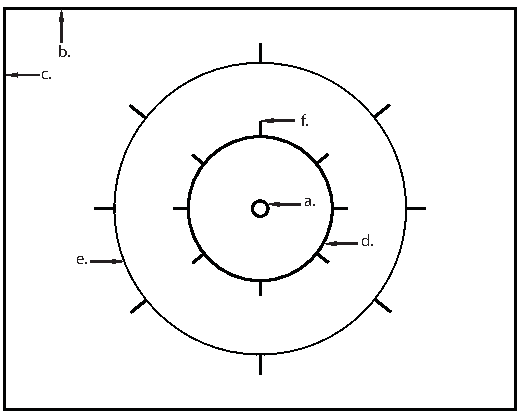
\includegraphics{std_skill_pattern_labeled}
\end{center}
\vspace{-20pt}
\caption{Riding Area Boundaries \label{fig:std_skill_pattern_labeled}}
\vspace{-10pt}
\end{figure}

\begin{enumerate}[a.]
\item Center circle (50cm diameter)
\item Long edge of riding area (faces judges)
\item Short edge of riding area
\item Inner circle (4m diameter) for circle figures
\item Outer circle (8m diameter) for line and figure eights.
\item Quarter and diagonal circle marks (length 1m) on the 4m and 8m circles.
Diagonals marked by going from corner to corner of the riding boundary.
\end{enumerate}


\subsection{Line Figure}
\begin{wrapfigure}{r}{0.35\textwidth}
\vspace{-35pt}
\begin{center}
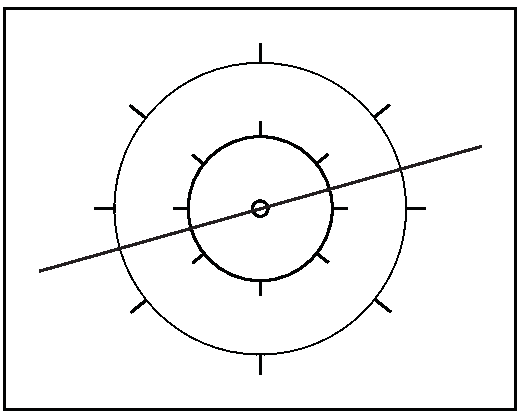
\includegraphics[width=0.33\textwidth]{std_skill_line_figure}
\end{center}
\vspace{-20pt}
\caption{Line Figure\label{fig:std_skill_line_figure}}
\vspace{-10pt}
\end{wrapfigure}
Lines, circles and figure eights may be ridden in any direction.
Line figures start outside the large (8m) circle, cross the center circle, and continue outside the large circle.
The rider must be in position for the figure before the hub crosses over the outside edge of the line.
For seat drag figures where the seat is forward of the riding direction, the rider must be in position before the seat crosses the outside edge of the line.
The line should be straight.
Circles and figure eights can be started at any point, as long as the rider completes the figure by crossing over the starting point.

\subsection{Circle Figure}
\begin{wrapfigure}{r}{0.35\textwidth}
\vspace{-75pt}
\begin{center}
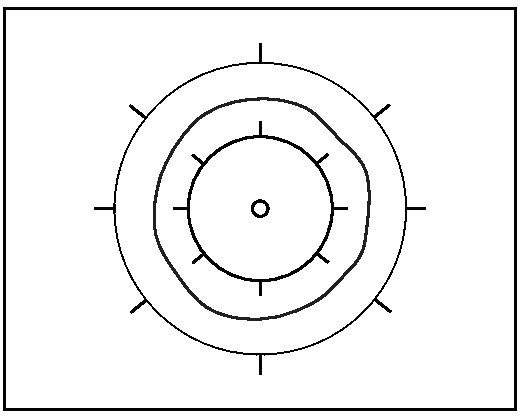
\includegraphics[width=0.33\textwidth]{std_skill_circle_figure}
\end{center}
\vspace{-20pt}
\caption{Circle Figure\label{fig:std_skill_circle_figure}}
\vspace{-10pt}
\end{wrapfigure}
Circle figures are ridden in the area between the 4m and 8m circle lines.
If the rider crosses the 4m line while performing the figure, the circle must be restarted from the point where the rider re-crosses to the outside of the 4m circle.
Crossing the 8m line does not invalidate the figure.
Circle figures should be as round as possible.

\subsection{Figure Eight}
\begin{wrapfigure}{r}{0.35\textwidth}
\vspace{-45pt}
\begin{center}
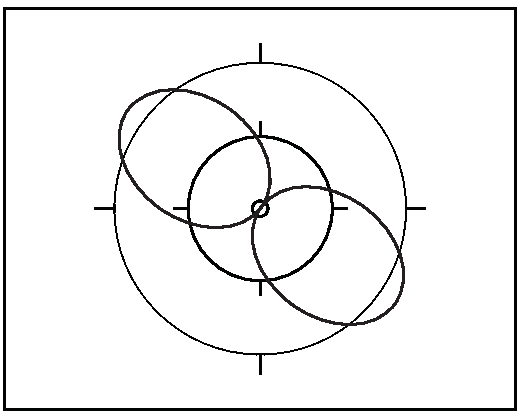
\includegraphics[width=0.33\textwidth]{std_skill_figure_eight}
\end{center}
\vspace{-20pt}
\caption{Figure Eight\label{fig:std_skill_figure_eight}}
\vspace{-10pt}
\end{wrapfigure}
The two circles making up the 8 should be the same size, and the orientation of the 8 can be in any direction.
The rider must pass outside the 8m circle on each end of the 8, and cross the center circle at the middle.
The two halves of the figure 8 must be circular, with diameters of at least 4m.

\section{Mounts, Transitions, Axis, Single And Counted Short Skills}
These are all collectively called ``non-riding skills''.
May be performed anywhere in the riding area unless stated differently in the description.

\section{Body Form}
Unless otherwise noted, each figure must be performed with riders sitting up straight with their arms stretched and horizontal.
Hands must be flat with palms down and fingers together.
Arms do not have to be straight out to the sides.
As long as arms are outstretched and horizontal, they may point in any direction.

\section{Dismounts}
All dismounts must be controlled, including the dismount at the end of the routine.
A controlled (intentional) dismount is where the rider comes to a stop and steps off the unicycle.
Dismounts executed otherwise will be considered unintentional.
A dismount occurs any time a rider touches the floor, except in skills where the rider is required to touch the floor, or when a foot on a pedal touches the floor.
The rules demand that the rider dismounts in a sportsmanlike manner at the end of the routine.
Failure to do so will result in a wave for insecure exit.

\section{Assisting Riders}
At international events it is forbidden for a rider to get verbal assistance or helping gestures from a person outside the riding area, since this is interference with the rider by an outside person.
At international events it is forbidden for a rider to use any props (including people) during the 3-minute routine.
Any competitor caught getting assistance (verbal or nonverbal) or using props may be disqualified from the competition.
Also, a rider may not look at the list of skills while performing the routine.
This includes skills written on the competitor's hand, a piece of paper or elsewhere.
Each occurrence of a competitor looking at a skills list will result in a wave.

\section{Standard Skill Judging Sheet}
Before competing in Standard Skill, each rider must fill out and turn in a judging sheet listing his or her routine.
This list includes the number, name, and point value of each figure to be performed in the routine, in the order in which they will be ridden.

\subsection{Skills To Be Used}
The maximum number of figures allowed is 18.
Of those 18 figures, no more than 12 may be other than a riding skill.
Skills with numbers 101 and higher are limited to a maximum of 12.
If a rider only chooses 12 skills for the whole routine, it is allowed for all of these to be non-riding skills.

\textbf{Note:} Each figure number may appear only once on the judging sheet.
This means that, for example, if a rider uses figure 15 b, he or she may not use 15 a, c, d, e, f, g, or h.

\subsection{Skill Order}
The 18 figures must be performed in the exact same order as they appear on the judging sheet.
Figures left out according to their order on the judging sheet will be devaluated 100\%.
This devaluation remains, even if the figure is performed later in the routine.
\textbf{Example:} The skills on a judging sheet are: wheel walk, one-foot, idle, riding backwards.
The rider does the wheel walk, skips the one-foot and idle, then performs the riding backwards, followed by the one-foot and the idle.
The technical judge will mark both the 1-ft and idle with a 100\% devaluation.

\subsection{Filling Out Judging Sheet}
The completed judging sheet must be sent in before the deadline date set by competition organizers.
When filling out the sheet, each figure name must be written out exactly as it appears on the Standard Skill List, with no further abbreviations.
Figure numbers, letters, and point values must be included, and the total Difficulty score (total points for all figures in the routine) must be filled in.
The judges have to check the judging sheets and, if possible in contact with the competitor, correct any mistakes.
Any disadvantage resulting from filling out a judging sheet incorrectly will be at the competitor's expense, and will not be valid grounds for protest.
Judging sheets, once checked and approved for competition, cannot be changed.

\subsection{Competitor and Judging Forms}
If available to the organizers, a computer database should be used to generate forms for both the competitor and the judges, and then be used to calculate the scores.
Either the Writing Judge Form or the traditional Standard Skill Form is required for judging.
The other forms are suggested to help both the competitors and judges.
Suggested forms are: 
\begin{itemize}
\item \textbf{Competitor Form:} Skill Order, Figure number and letter, Description, Score, and Skill Definition.
\item \textbf{Standard Skill Form:} Skill Order, Figure number and letter, Description, Score, and areas to mark 50/100\% technical devaluations and the ~ / + 0 execution devaluations.
An area at the bottom should be included to write in the names of the three judges.
An area at the bottom should also be included to help in manual scoring of the routines.
\item \textbf{Writing Judge Form:} Skill Order, Figure number and letter, Description, Score, and areas to mark 50/100\% technical devaluations and the ~ / + 0 execution devaluations.
An area at the bottom should be included to write in the names of the three judges.
\item \textbf{Difficulty Judge Form:} Skill Order, Figure number and letter, Description, Score, Skill Definition, and area to mark 50/100\% technical devaluations.
The addition of the Skill Definition can help the judge if there is clarification needed for the correct execution of the skill.
\item \textbf{Execution Judge Form:} Skill Order, Figure number and letter, Description, Score, and area to mark the ~ / + 0 execution devaluations.
\end{itemize}

All three judging forms should have grey shading to indicate the relative speed of the skills.
No shading would indicate a slower skill (typically all riding skills), a light grey indicates skills that are quicker than the riding skills (most of the counted short skills), and a dark grey indicates skills that are very quick.
This will help the judges estimate how quickly they must watch for new skills.

\chapter{Standard Skill Judging}

\section{Judging Panel \label{sec:freestyle_std-judging-panel}}
There will be 1 Chief Judge, 2 Difficulty Judges, 2 Execution Judges, 2 Writing Judges, and 1 Timer.
The judging panel will be divided into two judging units, each consisting of one Difficulty, one Execution, and one Writing Judge.
The judges will be appointed to the functions Writer, Execution, and Difficulty, respectively in order of their experience.
At Unicons, all judges for the Expert groups must have previous Unicon judging experience.

\section{Operation Of The Judges}
While the Difficulty and Execution Judges watch the routine, the Writing Judge reads the names of the figures from the list.
The Difficulty Judge indicates if a skill was fully completed, or the reduction percentage if it was not.
The Execution Judge indicates the execution mistakes using symbols, as described below.
The Writer writes down the verbal remarks of both judges on the judging sheet.
For this reason, the Writer is seated between the other two judges.
The position of the judging table must be so that all judges have a clear view of the entire riding area.
There must be enough space between the two judging units to ensure their working independently of each other.

A video of the performance may be reviewed if there are discrepancies in judge scores, or if a judge is in doubt about one or more of his/her scores.
When time allows, video can be reviewed by approval of the Chief Judge.
The Chief Judge should prearrange for routines to be recorded, but this is not a mandatory requirement.

Alternatively, to speed up the competition and judging, video cameras should be used to record the competition.
There must be at least two cameras, one on each of the two corners.
A third camera in the center is also good for a backup.
The recordings should be downloaded to a computer in approximately groups of ten competitors.
The judges will all be in a separate viewing area to watch the videos and make their scores.

\section{Difficulty Devaluations}

\subsection{Skill Verification}
Every figure on the judging sheet must be executed according to its description in the Standard Skill List.
If a performed figure does not correspond with the entry on the judging sheet, 100\% is devaluated.

\subsection{Technical Mistakes}
If a technical mistake occurs during the execution of a skill, 50\% is devaluated.
Technical mistakes include but are not limited to the following: 
\begin{itemize}
\item Part of body other than one hand touching seat in seat out skills
\item Hand holding seat touching body in seat out skills
\item Free foot touching rotating part of unicycle in one foot skills
\item Legs not extended and/or toe not pointed for skills where the leg is quickly extended (including, but not limited to: wheel grab, crank idle kick, hop on wheel kick)
\end{itemize}

\subsection{Skill Completion \label{subsec:freestyle_difficulty-devaluations_skill-completion}}
Every figure on the judging sheet must be performed as entered, from start to finish, without the rider touching the floor, except where required to by the figure description.
This applies to all skills: riding skills (figures in lines, circles and 8's), transitions, axis skills, single and counted short skills, and mounts.

\begin{wrapfigure}{l}{0.35\textwidth}
\vspace{-25pt}
\begin{center}
\includegraphics[width=0.33\textwidth]{std_skill_error_1}
\end{center}
\vspace{-20pt}
\caption{50\% Devaluation \label{fig:std_skill_error_1}}
\vspace{-5pt}
\begin{center}
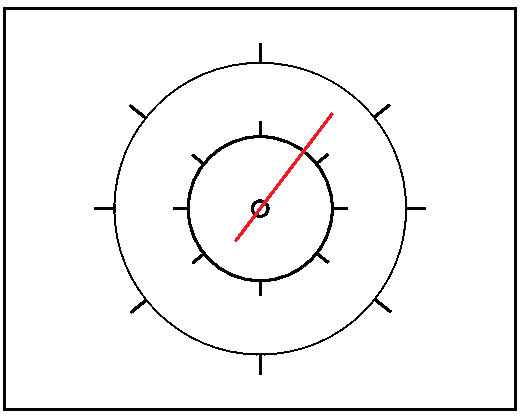
\includegraphics[width=0.33\textwidth]{std_skill_error_2}
\end{center}
\vspace{-20pt}
\caption{100\% Devaluation\label{fig:std_skill_error_2}}
\vspace{-25pt}
\end{wrapfigure}

\textbf{Riding Skills, Repetitive Axis Skills, and Counted Short Skills:} If a figure is broken off in the first half of its required execution, or performed for less than half of the required execution, 100\% is devaluated.
If a figure is broken off in the second half of the required execution, or performed for less than the required execution, 50\% is devaluated.

\textbf{Riding Skills:}
If a rider is not in position for a line figure before crossing the 8-meter circle, but is in position when crossing both 4-meter circle lines, 50\% is devaluated (see figure \ref{fig:std_skill_error_1}).
If the rider is in position but only crosses one edge of the 4-meter circle, 100\% is devaluated (see figure \ref{fig:std_skill_error_2}).

\textbf{Transitions and mounts:} Must finish in the end position (one revolution, $2 \frac{1}{2}$ hops, or $2 \frac{1}{2}$ idles) or 100\% is devaluated.
If the end position for a mount is not defined, must perform one revolution, OR $2 \frac{1}{2}$ hops, OR $2 \frac{1}{2}$ idles before stepping off the unicycle.

\textbf{Axis skills:} If the end position for a axis skill is not defined, must perform one revolution before stepping off the unicycle.
The ending position is not required to be the same as the starting position.

\textbf{Single Short Skills:} Unless otherwise defined in the skill description, the ending position is the same as the starting position.
Must finish in the end position (one revolution, $2 \frac{1}{2}$ hops, or $2 \frac{1}{2}$ idles) or 100\% is devaluated.
If the start and end position for a single short skill is not defined, must perform one revolution, $2 \frac{1}{2}$ hops, OR $2 \frac{1}{2}$ idles before stepping off the unicycle.

\subsection{Start Of Figures}
All figures start when the rider gets into the position required for that figure.

\subsection{Figure Order}
Figures left out according to their order on the judging sheet are devaluated 100\%.
This devaluation remains, even if the figure is performed afterward.

\subsection{Figure Patterns}
Riding figures that the rider doesn't attempt to be ridden as described in section \ref{subsec:freestyle_floor-markings-figure-shapes_riding-area-boundaries} should receive 100\% devaluation.

\textbf{Example:} The line figure is described as ``…start outside the large (8m) circle, cross the center circle, and continue outside the large circle''.
If the rider does not attempt to cross the center circle and performs the line circle completely outside the 4m circle, then 100\% is devaluated.

\section{Execution Devaluations}

\subsection{Wave (~) = -0.5 Point}
A wave is scored once per skill for each of the following execution mistakes listed below.
More than one wave can be applied to each skill, but if a rider makes the same mistake twice during one skill, they should only receive one wave.

\textbf{Example:} During wheel walking, a rider may have jerky body movements and fingers not together at the beginning – two waves should be applied.
If the rider then smoothly wheel walks for a while and then has jerky body movements again, a third wave should not be applied.
\begin{itemize}
\item insecure entrance or exit 
\item cramped, insecure execution 
\item jerky body movements 
\item not sitting up straight 
\item fingers not together 
\item free leg not stretched, toes not pointed 
\item waving arms 
\item jerky pedal movement 
\item line not straight 
\item circle not round 
\item crossing the 4 m circle when performing a skill in a circle 
\item failure to cross center circle in line or figure 8 
\item circles of figure 8 not the same size 
\item pedal, or foot on pedal touching floor 
\item wandering spin or pirouette 
\item circle size exceeds 1 meter diameter in a spin 
\item going outside riding area boundary 
\item looking at the standard skill order 
\item arms not stretched 
\item arms not horizontal 
\item palms not down 
\item arms touching the body during seat out skills
\end{itemize}

\subsection{Line (/) = - 1 Point}
A line is scored every time loss of control occurs.
Loss of control includes:
\begin{itemize}
\item loss of proper body form 
\item breaking off and restarting a skill 
\item loss of proper body form before or after transitions
\end{itemize}

\subsection{Cross (+) = - 2 Points}
A cross is scored each time an unintentional dismount occurs with the competitor landing on his or her feet without the unicycle being dropped.

\subsection{Circle (0) = - 3 Points}
A circle is scored each time an unintentional dismount occurs with a part of the rider other than his or her feet touching the floor (hand, knee, rear, etc.) or with the unicycle being dropped.
Seat drag skills only have this score applied if a part of the rider other than the feet touches the floor.

\subsection{Applying Lines, Circles, Crosses}
Lines, circles and crosses are scored every time they occur during and between all skills, whether entered on the score sheet or not.
Only the highest applicable devaluation symbol shall be imposed per execution mistake.
Most waves are not scored if they occur between skills listed on the judging sheet.
Waves can only be scored between skills if they are unrelated to body form.

\textbf{Example:} A competitor will not get a wave if the competitor's arms are not in proper form between skills listed on the judging sheet, but a competitor will get a wave for exceeding the riding area boundary.

\section{Totaling Scores}
After the routine is finished, the percentages and symbols from the judges are converted into numbers.
These numbers are subtracted from the rider's starting score.
Then, the scores of the two judging units are added together and divided by two to get the finishing score of a competitor.
The winner in the Standard Skill event is the competitor with the highest score.
If more than one competitor have the same score, placing is decided by the highest Execution score.
If those scores are also the same, the competitors receive tie scores.

\documentclass[a4paper,oneside,parskip=half,numbers=noenddot]{scrbook}


%%% Page Layout %%%
\textwidth=14.7cm % these two commands make the page fit in a box 
\textheight=22.1cm % ... that works on both letter and A4 paper
%\hoffset=5.8754pt % enable if using letterpaper to center document on page


%%% Preamble things that must happen first %%%


%%% Basic Setup %%%
\pdfminorversion=7 % use a more current pdf version to support better graphics inclusions


%%% Language support %%%
\usepackage[utf8]{inputenc} % use utf-8 encoding for better language support
\usepackage[T1]{fontenc} % uses 8-bit font encoding for better character support
\usepackage{lmodern} % use lmodern font for better character support and a prettier font


%%% Additional Simple Packages %%%
\usepackage{color} % for latexdiff
\usepackage[normalem]{ulem} % for latexdiff


%%% Graphics Packages %%%
\usepackage{graphicx}
\graphicspath{{img/}{./img/}{src/img/}}
\usepackage{wrapfig}
\usepackage{pict2e}


%%% User defined commands and associated packages %%%
\usepackage{comment}
\excludecomment{comment2016}

\newcommand{\unit}[1]{\ensuremath{\, \mathrm{#1}}} % use \unit{km} in math mode for better units

\usepackage{framed}
\newcommand{\oldrule}[1]{} % don't display oldrule (next line is displayed oldrule)
%\newcommand{\oldrule}[1]{\framebox{#1}} % displays oldrule references in a nice box


%%% GitInfo %%%
\usepackage{gitinfo2}
% gitinfo2 package can be found in the dependencies directory
% git hooks must also be installed and these are found in the scripts directory


%%% Tabular environment changes and packages %%%
\usepackage{array} % basic table package, "a must use"
\usepackage{longtable}
\usepackage{multicol}
\usepackage{multirow}

\newcolumntype{P}[1]{>{\raggedright\arraybackslash}p{#1}} % use column type 'P' instead of 'p' for non-justified paragraph text in a table - used primarily in the freestyle judging sections


%%% Additional basic custimizations %%%
\renewcommand{\thepart}{\arabic{part}} % arabic part numbering
\renewcommand{\thechapter}{\arabic{part}\Alph{chapter}} % make chapters numbered with part and then letter
%\renewcommand{\thesection}{\arabic{part}.\arabic{section}} % replace chapter number with part number in sections %% used prior to reorg

\setcounter{secnumdepth}{3} % makes subsubsections numbered

\usepackage[shortlabels]{enumitem} % allows list customization here below
\setlist{itemsep=-1mm, topsep=-1pt, partopsep=0pt} % customize spacing around lists

\newlist{judging_items}{itemize}{1} %redefine itemize for the freestyle judging grid to fit
\setlist[judging_items]{label=\textbullet,leftmargin=*, labelsep=0.7mm,itemsep=-1mm, topsep=-6pt, partopsep=-5pt}


\RedeclareSectionCommands[
  beforeskip=-\baselineskip,
  afterskip=.5\baselineskip]{section,subsection,subsubsection}
% this command is supposed to replace titlesec's titlespacing option
% the desired before/after spacing was {12pt plus 4pt minus 2pt}{0pt plus 2pt minus 2pt}




%%% Customize Part/Chapter/Section/Page numbering %%%
\usepackage{remreset} % allows the resets here below
\makeatletter
\@addtoreset{chapter}{part} % reset chapter numbering for each part
\@addtoreset{section}{part} % reset section numbering for each part
%\@removefromreset{section}{chapter} % don't reset section numbering in new chapters
\makeatother

%don't reset page numbers ever (specifically not after frontmatter)
\makeatletter
\def\pagenumbering#1{%
  \gdef\thepage{\csname @#1\endcsname \c@page}}
\makeatother


%%% Headings %%%
\usepackage[markcase=ignoreuppercase,autooneside]{scrlayer-scrpage} %better headings without uppercase TOC heading
\pagestyle{scrheadings}
\clearscrheadfoot %clear all header and footer styles to allow custimization
\cfoot[\pagemark]{\pagemark} %pagenumbers in footer
\makeatletter
\let\Oldpart\part
\newcommand{\parttitle}{}
\renewcommand{\part}[1]{\Oldpart{#1}\renewcommand{\parttitle}{#1}}
\renewcommand{\chaptermark}[1]{\markboth{#1}{}}
\renewcommand*{\chapterpagestyle}{headings} %display headers on first page of chapters

\chead[]{
  \ifnum\value{chapter}>0
    \thepart \ \parttitle -- \leftmark
  \else
    \thepart \ \parttitle 
  \fi
  }
\makeatother


%%% Hyperref %%%
% must be loaded as late as possible in preamble, with a few things after
\usepackage{hyperref} % clickable table of contents, index in pdf files 
\hypersetup{
    colorlinks,
    citecolor=black,
    filecolor=black,
    linkcolor=black,
    urlcolor=black
}


%%% Must be loaded after hyperref %%%
\usepackage[numbered]{bookmark} % customize PDF bookmarks 
\usepackage{minitoc} % for table of contents per part


%%% TOC custimization %%%
%% all of this comes after minitoc is loaded %%
\setcounter{tocdepth}{-1} % only includes parts and chapters (not sections) in main TOC
\mtcsetdepth{parttoc}{1} % only includes chapters and sections (not subsections) in part TOCs

\usepackage[tocindentauto]{tocstyle} % prettier TOC
\usetocstyle{allwithdot} %use 'KOMAlike" if you don't want dots
\settocstylefeature [-1] {entryvskip} {15pt}
\settocstylefeature [0] {entryvskip} {10pt}
\settocstylefeature [0] {entryhook} {\hspace{18pt} }

\renewcommand{\mtcgapbeforeheads}{0pt}
\renewcommand{\mtcgapafterheads}{0pt}
\mtcsettitle{parttoc}{Contents} %renames the part TOC to match main TOC

\usepackage{tocloft} % package for below command
\renewcommand{\cftsecnumwidth}{3em} %changes spacing between number and name on sections in TOC (and minitocs) to help with long section numbers (i.e. 1C.14)

\renewcommand{\thesection}{\arabic{part}\alph{chapter}.\arabic{section}} % replace chapter number with part number in sections

\begin{document}

\begin{titlepage}
\centering
\ \\
\vspace{5cm}
{\Huge IUF Standard Skills List}
\vspace{5mm}


\includegraphics{../img/iuf-logo}

\vspace{5mm}
{\huge International Unicycling Federation}

\vspace{70mm}
Prepared by the IUF Rulebook Committee.

\vspace{5mm}
{\small Copyright \copyright\ 2015 by the International Unicycling Federation, Inc. All rights reserved.} \\
\small{Last Revision 2012.}

\end{titlepage}

\setcounter{chapter}{5}\setcounter{part}{6}
\chapter{List of Standard Skills \label{chap:freestyle_std-skills-list}}

\section{General Remarks About Standard Skill Riding  }
Only figures listed in the following skills list can be used for the assembly of Standard Skill routines.

\subsection{Riding Position}
Unless stated differently in a figure description, it is to be executed with the rider seated and with both feet on the pedals.

\subsection{Body Form}
The rider must show proper body form and shall not change this form during the execution of the entire figure.
Proper body form must also be shown for the figure before and after transitions, even if not listed on the judging sheet.
The body form may be relaxed when not performing figures, except for figures before and after transitions.

\subsection{Riding Direction}
Unless stated differently, all riding figures are to be performed riding forward, this being the direction in which the rider faces.

\subsection{Pattern}
Unless stated differently in a figure description, it is to be executed in a line.
Exceptions are mounts, stationary skills and transitions, axis skills, single and counted short skills, which can be executed at any spot in the riding area.

\subsection{Transitions, And Single Short Skills}
Unless stated differently in the description of a transition, it starts and ends with the rider seated with both feet on the pedals.
Before and after transitions, and single short skills entered on the score sheet as figures, at least one revolution of the wheel must be ridden in the start and end positions.
If the start or end position of a transition or single short skill is a counted short skill, that skill must be executed at least 50\% as described, whether or not it is listed on the judging sheet.

\textbf{Example 1:} For the transition ``Riding to Seat in Front'', the rider must ride at least one full revolution of the wheel with the seat in front.

\textbf{Example 2:} For the single short skill, 180$^\circ$ uni spin to idling 1ft, the rider must idle one foot $2 \frac{1}{2}$ cycles.

\subsection{Axis Skills}
Unless stated differently in the description, it starts and ends with the rider seated with both feet on the pedals.
Before axis skills entered on the score sheet as figures, at least one revolution of the wheel must be ridden in the start position.
After axis skills, at least one revolution of the wheel must be ridden.
The ending position is not required to be the same as the starting position.

\subsection{Mounts}
Unless stated differently in the description of a mount, it is to end with the rider seated with both feet on the pedals.
After all mounts listed on the judging sheet as figures, at least one full revolution of the wheel must be ridden in the end position.
For mounts ending in counted short skills, the skill must be executed at least 50\% as described, whether or not it is listed on the judging sheet.

\textbf{Example:} For the Side Mount, the rider must ride at least one full revolution of the wheel in the riding position after mounting.

\subsection{Seat Out Figures}
Unless stated differently in seat out figures, the rider shall have no contact with the seat other than one hand holding the seat.
The hand holding the seat as well as the corresponding arm shall be extended away from the rider's body and shall not touch any part of the rider's body.

\subsection{One Foot Figures}
Unless stated differently in one foot figures, the free foot is to be placed on the frame so that there is no contact between the free foot and any rotating part of the unicycle.

\subsection{Wheel Walk Figures}
Unless stated differently in wheel walk figures, the feet are to push only the tire, and shall have no contact with the pedals or crank arms.

\subsection{Coasting}
Unless stated differently in coasting figures, the feet are to have no contact with any rotating part of the unicycle (pedals, crank arms, or tire).

\subsection{Transitions, Single Short Skills, Mounts Involving Seat Out Skills}
Unless stated differently in the description of the figure, those beginning or ending in seat out skills are allowed to have one or both hands touching the seat, and the seat touching the body for the final or first hop, idle, or revolution.
This includes, but is not limited to: unispins to seat out skills, transitions into and out of seat in front or back, leg around skills, side ride to seat in front, transitions out of seat drag in front or back, hopping wheel to pedals.

\subsection{Transitions To/From Stand Up Wheel Walk}
In all transition skills from/to stand up wheel walk position, a second foot may briefly touch the wheel during the transition, but only one foot pushes the wheel forward.
Unless clearly stated in the description, the rider must perform stand up wheel walk forward.

\subsection{Spins And Pirouettes}
The rider must make a minimum of three full rotations for spins and pirouettes.
Spins must be ridden around a fixed point and must not exceed a 1 meter diameter.
If rider rotates more than required minimum number, the last required rotations are judged for spins.
Pirouettes must be executed on 1 spot and the pedals may not move backward or forward during the pirouette.
If rider rotates more than required minimum number, the first required rotations are judged for pirouettes.

\subsection{Leg Around Skills}
All variations may begin or end with feet on the cranks or pedals and begin or end either riding, idling, or hopping unless otherwise specified.

\subsection{Idling Figures}
In idling figures, a minimum of 5 consecutive cycles (back and forth motions) must be executed.

\subsection{Twisting Figures}
In twisting figures, a minimum of 5 consecutive cycles (side to side motions) must be executed.

\subsection{Stillstands}
The minimum time for stillstands is 3 seconds.

\subsection{Hopping Figures}
In hopping figures, a minimum of 5 consecutive hops must be executed.

\section{Standard Skill Scores and Descriptions}
The following descriptions are meant to explain the correct way to execute the skills.
Any illustrations are intended to clarify the descriptions.
If illustrations and descriptions disagree, the descriptions always apply.

\textbf{Abbreviations Used In This List:}
\begin{center}
\begin{tabular}{l l l p{2cm} l l l}
fwd & = & forward & & c & = & circle \\
ext & = & extended & & 1ft & = & one foot \\
bwd & = & backward & & 8 & = & figure eight \\
frh & = & freehand & & ww & = & wheel walk \\
\end{tabular}
\end{center}
\newpage

\subsection{Riding Skills}
\renewcommand{\arraystretch}{1.5}
\begin{longtable}{|r|c|p{4cm}|p{8cm}|c|}
\hline
1 & a & riding  & Riding (sitting on seat, facing forward). & 1.0 \\ 
\hline
  & b & riding - c  & Riding in a circle (sitting on seat, facing forward). & 1.3 \\ 
\hline
  & c & riding - 8  & Riding in a figure eight sitting on seat, facing forward).  & 1.5 \\ 
\hline
2 & a & riding holding seatpost, 1 hand & Riding while leaning forward and with one hand holding the seatpost under the seat. & 1.3 \\ 
\hline
  & b & riding holding seatpost, 1 hand - c & Riding in a circle while leaning forward and with one hand holding the seatpost under the seat. & 1.6 \\ 
\hline
  & c & riding holding seatpost, 1 hand - 8 & Riding in a figure 8 while leaning forward and with one hand holding the seatpost under the seat. & 1.9 \\ 
\hline
  & d & riding holding seatpost, 2 hands  & Riding while leaning forward and with both hands holding the seatpost under the seat. & 1.4 \\ 
\hline
  & e & riding holding seatpost, 2 hands - c  & Riding in a circle while leaning forward and with both hands holding the seatpost under the seat. & 1.8 \\ 
\hline
  & f & riding holding seatpost, 2 hands - 8  & Riding in a figure 8 while leaning forward and with both hands holding the seatpost under the seat. & 2.0 \\ 
\hline
3 & a & riding bwd  & Riding backward.  & 2.5 \\ 
\hline
  & b & riding bwd - c  & Riding in a circle backward.  & 3.1 \\ 
\hline
  & c & riding bwd - 8  & Riding backward in a figure eight.  & 3.6 \\ 
\hline
4 & a & seat in front, seat against body  & Riding with seat held in front of the rider. The seat or hand holding the seat may rest against the rider.  & 2.0 \\ 
\hline
  & b & seat in front & Riding with seat held in front of the rider.  & 2.3 \\ 
\hline
  & c & seat in front - c & Riding in a circle with seat held in front of the rider.  & 2.9 \\ 
\hline
  & d & seat in front - 8 & Riding in a figure eight with seat held in front of the rider.  & 3.3 \\ 
\hline
  & e & seat in front frh, seat against body  & Riding with seat held out in front of the rider. Neither hand touches the seat and the seat post is held between the rider's legs. The seat may rest against the rider. & 3.3 \\ 
\hline
  & f & seat in front frh & Riding with seat held in front of the rider. Neither hand touches the seat and the seat post is held between the rider's legs.  & 3.7 \\ 
\hline
  & g & seat in front frh - c & Riding in a circle with seat held in front of the rider. Neither hand touches the seat and the seat post is held between the rider's legs.  & 4.3 \\ 
\hline
  & h & seat in front frh - 8 & Riding in a figure eight with seat held in front of the rider. Neither hand touches the seat and the seat post is held between the rider's legs.  & 4.8 \\ 
\hline
5 & a & seat in front bwd, seat against body  & Riding backward with seat held out in front of the rider. The seat or hand holding the seat may rest against the rider. & 3.4 \\ 
\hline
  & b & seat in front bwd & Riding backward with seat held out in front of the rider. & 3.6 \\ 
\hline
  & c & seat in front bwd - c & Riding backward in a circle with seat held out in front of the rider. & 4.1 \\ 
\hline
  & d & seat in front bwd - 8 & Riding backward in a figure eight with seat held out in front of the rider. & 4.7 \\ 
\hline
  & e & seat in front bwd frh, seat against body  & Riding backward with seat held out in front of the rider. Neither hand touches the seat and the seat post is held between the rider's legs. The seat may rest against the rider.  & 4.0 \\ 
\hline
  & f & seat in front bwd frh & Riding backward with seat held out in front of the rider. Neither hand touches the seat and the seat post is held between the rider's legs. & 4.5 \\ 
\hline
  & g & seat in front bwd frh - c & Riding backward in a circle with seat held out in front of the rider. Neither hand touches the seat and the seat post is held between the rider's legs. & 5.2 \\ 
\hline
6 & a & seat in back, seat against body & Riding with the seat held out behind the rider. The seat or the hand holding the seat may rest against the rider. & 2.2 \\ 
\hline
  & b & seat in back  & Riding with the seat held out behind the rider. & 2.5 \\ 
\hline
  & c & seat in back - c  & Riding in a circle with the seat held out behind the rider. & 3.1 \\ 
\hline
  & d & seat in back - 8  & Riding in a figure eight with the seat held out behind the rider. & 3.6 \\ 
\hline
7 & a & seat in back bwd, seat against body & Riding backward with the seat held out behind the rider. The seat or the hand holding the seat may rest against the rider.  & 3.5 \\ 
\hline
  & b & seat in back bwd  & Riding backward with the seat held out behind the rider.  & 3.9 \\ 
\hline
  & c & seat in back bwd - c  & Riding backward in a circle with the seat held out behind the rider.  & 4.5 \\ 
\hline
  & d & seat in back bwd - 8  & Riding backward in a figure eight with the seat held out behind the rider.  & 5.1 \\ 
\hline
8 & a & seat on side, seat against body & Riding with the seat held out to the side of the rider. The seat or the hand holding the seat may rest against the rider. & 3.4 \\ 
\hline
  & b & seat on side, seat against body - c & Riding in a circle with the seat held out to the side of the rider. The seat or the hand holding the seat may rest against the rider. & 3.2 \\ 
\hline
  & c & seat on side  & Riding with the seat held out to the side of the rider. & 4.1 \\ 
\hline
  & d & seat on side - c  & Riding in a circle with the seat held out to the side of the rider. & 3.9 \\ 
\hline
9 & a & seat on side bwd, seat against body & Riding backward with the seat held out to the side of the rider. The seat or the hand holding the seat may rest against the rider.  & 4.3 \\ 
\hline
  & b & seat on side bwd  & Riding backward with the seat held out to the side of the rider.  & 4.6 \\ 
\hline
  & c & seat on side bwd - c  & Riding backward in a circle with the seat held out to the side of the rider.  & 4.4 \\ 
\hline
10  & a & stomach on seat, 1 hand on seat & Riding with the abdomen on the seat. One hand holds onto the seat.  & 2.1 \\ 
\hline
  & b & stomach on seat & Riding with the abdomen on the seat, frh. & 2.3 \\ 
\hline
  & c & stomach on seat - c & Riding in a circle with the abdomen on the seat, frh. & 2.9 \\ 
\hline
  & d & stomach on seat - 8 & Riding in a figure eight with the abdomen on the seat, frh. & 3.3 \\ 
\hline
11  & a & stomach on seat bwd & Riding backward with the abdomen on the seat, hands free. & 3.8 \\ 
\hline
  & b & stomach on seat bwd - c & Riding backward in a circle with the abdomen on the seat, hands free. & 4.4 \\ 
\hline
  & c & stomach on seat bwd - 8 & Riding backward in a figure eight with the abdomen on the seat, hands free. & 4.9 \\ 
\hline
12  & a & chin on seat, 1 hand on seat  & Riding with no part of the body other than the chin touching the back of the seat. One hand may touch the seat. & 3.5 \\ 
\hline
  & b & chin on seat  & Riding with no part of the body other than the chin touching the back of the seat, freehanded.  & 4.0 \\ 
\hline
  & c & chin on seat - c  & Riding in a circle with no part of the body other than the chin touching the back of the seat, freehanded.  & 4.6 \\ 
\hline
  & d & chin on seat - 8  & Riding in a figure eight with no part of the body other than the chin touching the back of the seat, freehanded.  & 5.2 \\ 
\hline
13  & a & chin on seat bwd, 1 hand on seat  & Riding backward with no part of the body other than the chin touching the back of the seat, freehanded. One hand may touch the seat.  & 4.2 \\ 
\hline
  & b & chin on seat bwd  & Riding backward with no part of the body other than the chin touching the back of the seat, freehanded. & 4.9 \\ 
\hline
  & c & chin on seat bwd - c  & Riding backward in a circle with no part of the body other than the chin touching the back of the seat, freehanded. & 5.6 \\ 
\hline
  & d & chin on seat bwd - 8  & Riding backward in a figure eight with no part of the body other than the chin touching the back of the seat, freehanded. & 6.4 \\ 
\hline
14  & a & drag seat in front  & Riding with the seat dragging on the floor, in front of the wheel.  & 4.1 \\ 
\hline
  & b & drag seat in front - c  & Riding in a circle with the seat dragging on the floor, in front of the wheel.  & 4.7 \\ 
\hline
  & c & drag seat in front - 8  & Riding in a figure eight with the seat dragging on the floor, in front of the wheel.  & 5.3 \\ 
\hline
15  & a & drag seat in front bwd  & Riding backwards with the seat dragging on the floor, in front of the wheel.  & 5.3 \\ 
\hline
  & b & drag seat in front bwd - c  & Riding backwards in a circle with the seat dragging on the floor, in front of the wheel.  & 6.1 \\ 
\hline
  & c & drag seat in front bwd - 8  & Riding backwards in a figure eight with the seat dragging on the floor, in front of the wheel.  & 6.9 \\ 
\hline
16  & a & drag seat in back & Riding with the seat dragging on the floor, behind the wheel. & 4.3 \\ 
\hline
  & b & drag seat in back - c & Riding in a circle with the seat dragging on the floor, behind the wheel. & 4.9 \\ 
\hline
  & c & drag seat in back - 8 & Riding in a figure eight with the seat dragging on the floor, behind the wheel. & 5.6 \\ 
\hline
17  & a & drag seat in back bwd & Riding backward with the seat dragging on the floor, behind the wheel.  & 6.0 \\ 
\hline
  & b & drag seat in back bwd - c & Riding backward in a circle with the seat dragging on the floor, behind the wheel.  & 6.9 \\ 
\hline
  & c & drag seat in back bwd - 8 & Riding backward in a figure 8 with the seat dragging on the floor, behind the wheel.  & 7.8 \\ 
\hline
18  & a & riding sideways, seat against body  & Riding with the feet parallel to the wheel axle and the body turned 90 degrees to the riding direction with the seat in front holding with one or two hands. The seat or the hands holding the seat may touch the body. & 5.6 \\ 
\hline
  & b & riding sideways & Riding with the feet parallel to the wheel axle and the body turned 90 degrees to the riding direction with the seat in front holding with one or two hands.  & 5.7 \\ 
\hline
  & c & riding sideways 1ft ext, seat against body  & Riding with one foot parallel to the wheel axle and the body turned 90 degrees to the riding direction with the seat in front holding with one or two hands. The seat or the hands holding the seat may touch the body. The free leg is extended. & 6.0 \\ 
\hline
  & d & riding sideways seat drag & Riding seat drag in front (forward of the direction of travel) with the feet parallel to the wheel axle and the body turned 90 degrees to the riding direction. & 6.3 \\ 
\hline
19  & a & one foot  & Riding with one foot on pedal.  & 3.0 \\ 
\hline
  & b & one foot - c  & Riding in a circle with one foot on pedal.  & 3.5 \\ 
\hline
  & c & one foot - 8  & Riding in a figure eight with one foot on pedal.  & 3.9 \\ 
\hline
  & d & one foot ext  & Riding with one foot on pedal. The free leg is extended.  & 3.2 \\ 
\hline
  & e & one foot ext - c  & Riding in a circle with one foot on pedal. The free leg is extended.  & 3.7 \\ 
\hline
  & f & one foot ext - 8  & Riding in a figure eight with one foot on pedal. The free leg is extended.  & 4.2 \\ 
\hline
  & g & one foot crossed  & Riding with one foot on pedal. The free leg is crossed over the pedaling leg. & 3.4 \\ 
\hline
  & h & one foot crossed - c  & Riding in a circle with one foot on pedal. The free leg is crossed over the pedaling leg. & 3.9 \\ 
\hline
  & i & one foot crossed - 8  & Riding in a figure eight with one foot on pedal. The free leg is crossed over the pedaling leg. & 4.4 \\ 
\hline
20  & a & one foot bwd  & Riding backward with one foot on pedal. & 4.0 \\ 
\hline
  & b & one foot bwd - c  & Riding backward in a circle with one foot on pedal. & 4.6 \\ 
\hline
  & c & one foot bwd - 8  & Riding backward in a figure eight with one foot on pedal. & 5.2 \\ 
\hline
  & d & one foot ext bwd  & Riding backward with one foot on pedal. The free leg is extended. & 4.4 \\ 
\hline
  & e & one foot ext bwd - c  & Riding backward in a circle with one foot on pedal. The free leg is extended. & 5.1 \\ 
\hline
  & f & one foot ext bwd - 8  & Riding backward in a figure eight with one foot on pedal. The free leg is extended. & 5.7 \\ 
\hline
21  & a & one foot seat in front against body & Riding with the seat held out in front of the rider with ONE hand, one foot on pedal. The seat or hand holding the seat my rest against the rider.  & 3.8 \\ 
\hline
  & b & one foot seat in front  & Riding with the seat held out in front of the rider with ONE hand, one foot on pedal. & 4.5 \\ 
\hline
  & c & one foot seat in front - c  & Riding in a circle with the seat held out in front of the rider with ONE hand, one foot on pedal. & 5.2 \\ 
\hline
  & d & one foot seat in front - 8  & Riding in a figure eight with the seat held out in front of the rider with ONE hand, one foot on pedal. & 5.9 \\ 
\hline
  & e & one foot ext, seat in front against body  & Riding with the seat held out in front of the rider, one foot on pedal. The seat or hand holding the seat my rest against the rider. The free leg is extended.  & 4.1 \\ 
\hline
  & f & one foot ext, seat in front against body - c  & Riding in a circle with the seat held out in front of the rider, one foot on pedal. The seat or hand holding the seat my rest against the rider. The free leg is extended.  & 4.7 \\ 
\hline
22  & a & one foot seat in front against body bwd & Riding backward with the seat held out in front of the rider, one foot on pedal. The seat or hand holding the seat may rest against the rider.  & 4.7 \\ 
\hline
  & b & one foot seat in front bwd  & Riding backward with the seat held out in front of the rider, one foot on pedal.  & 5.4 \\ 
\hline
  & c & one foot seat in front bwd - c  & Riding backward in a circle with the seat held out in front of the rider, one foot on pedal.  & 6.2 \\ 
\hline
  & d & one foot ext, seat in front against body bwd  & Riding backward with the seat held out in front of the rider, one foot on pedal. The seat or hand holding the seat my rest against the rider. The free leg is extended. & 5.9 \\ 
\hline
  & e & one foot ext, seat in front against body bwd - c  & Riding backward in a circle with the seat held out in front of the rider, one foot on pedal. The seat or hand holding the seat my rest against the rider. The free leg is extended. & 6.8 \\ 
\hline
23  & a & seat on side, 1ft, seat against body  & Riding with the seat held out to the side of the rider, one foot on pedal. The seat or the hand holding the seat may rest against the rider.  & 4.0 \\ 
\hline
  & b & seat on side, 1ft & Riding with the seat held out to the side of the rider, one foot on pedal.  & 5.0 \\ 
\hline
  & c & seat on side, 1ft - c & Riding in a circle with the seat held out to the side of the rider, one foot on pedal.  & 4.8 \\ 
\hline
  & d & seat on side, 1ft - 8 & Riding in a figure eight with the seat held out to the side of the rider, one foot on pedal.  & 6.5 \\ 
\hline
24  & a & seat on side, 1ft bwd, seat against body  & Riding backward with the seat held out to the side of the rider, one foot on pedal. The seat or the hand holding the seat may rest against the rider. & 5.0 \\ 
\hline
  & b & seat on side, 1ft bwd & Riding backward with the seat held out to the side of the rider, one foot on pedal. & 5.4 \\ 
\hline
  & c & seat on side, 1ft bwd - c & Riding backward in a circle with the seat held out to the side of the rider, one foot on pedal. & 5.1 \\ 
\hline
25  & a & side saddle, hand touching seat & Riding 1ft while sitting partially on seat with the free leg resting on the seat or on the same side as the pedaling foot. One hand may touch the seat. & 3.5 \\ 
\hline
  & b & side saddle, hand touching seat - c & Riding 1 foot in a circle while sitting partially on seat with the free leg resting on the seat or on the same side as the pedaling foot. One hand may touch the seat.  & 4.0 \\ 
\hline
  & c & side saddle frh & Riding 1ft while sitting partially on seat with the free leg resting on the seat or on the same side as the pedaling foot.  & 3.7 \\ 
\hline
  & d & side saddle frh - c & Riding 1 foot in a circle while sitting partially on seat with the free leg resting on the seat or on the same side as the pedaling foot. & 4.3 \\ 
\hline
  & e & side saddle frh - 8 & Riding 1 foot in a figure eight while sitting partially on seat with the free leg resting on the seat or on the same side as the pedaling foot. & 4.8 \\ 
\hline
26  & a & cross over  & Riding one footed, with the pedaling foot on the non-corresponding pedal. Non pedaling foot can be extended, or on the fork.  & 4.4 \\ 
\hline
  & b & cross over - c  & Riding one footed in a circle, with the pedaling foot on the non-corresponding pedal. Non pedaling foot can be extended, or on the fork.  & 4.2 \\ 
\hline
  & c & cross over - 8  & Riding one footed in a figure eight, with the pedaling foot on the non-corresponding pedal. Non pedaling foot can be extended, or on the fork.  & 5.7 \\ 
\hline
27  & a & cross over bwd  & Riding backward one footed, with the pedaling foot on the non-corresponding pedal. Non pedaling foot can be extended, or on the fork. & 5.4 \\ 
\hline
  & b & cross over bwd - c  & Riding backward one footed in a circle, with the pedaling foot on the non-corresponding pedal. Non pedaling foot can be extended, or on the fork. & 5.1 \\ 
\hline
  & c & cross over bwd - 8  & Riding backward one footed in a figure 8, with the pedaling foot on the non-corresponding pedal. Non pedaling foot can be extended, or on the fork. & 7.0 \\ 
\hline
28  & a & side ride & Riding 1ft, next to the unicycle, with foot on the non-corresponding pedal, holding on to the seat with both hands. The seat or the hands holding the seat may rest against the rider.  & 5.9 \\ 
\hline
  & b & side ride - c & Riding 1 foot in a circle, next to the unicycle, with foot on the non-corresponding pedal, holding on to the seat with both hands. The seat or the hands holding the seat may rest against the rider. & 5.6 \\ 
\hline
  & c & side ride - 8 & Riding 1ft in a figure eight, next to the unicycle, with foot on the non-corresponding pedal, holding on to the seat with both hands. The seat or the hands holding the seat may rest against the rider.  & 7.7 \\ 
\hline
  & d & side ride, 1 hand & Riding 1ft, next to the unicycle, with foot on the non-corresponding pedal, holding on to the seat with one hand. The seat or the hand holding the seat may rest against the rider. & 6.2 \\ 
\hline
  & e & side ride, 1 hand - c & Riding 1ft in a circle, next to the unicycle, with foot on the non-corresponding pedal, holding on to the seat with one hand. The seat or the hand holding the seat may rest against the rider. & 5.9 \\ 
\hline
  & f & side ride, 1 hand - 8 & Riding 1ft in a figure eight, next to the unicycle, with foot on the non-corresponding pedal, holding on to the seat with one hand. The seat or the hand holding the seat may rest against the rider. & 8.1 \\ 
\hline
29  & a & side ride bwd & Riding 1ft bwd, next to the unicycle, with foot on the non-corresponding pedal, holding on to the seat with both hands. The seat or the hands holding the seat may rest against the rider.  & 6.6 \\ 
\hline
  & b & side ride bwd - c & Riding 1ft bwd in a circle, next to the unicycle, with foot on the non-corresponding pedal, holding on to the seat with both hands. The seat or the hands holding the seat may rest against the rider.  & 6.3 \\ 
\hline
  & c & side ride bwd - 8 & Riding 1ft bwd in a figure 8, next to the unicycle, with foot on the non-corresponding pedal, holding on to the seat with both hands. The seat or the hands holding the seat may rest against the rider.  & 8.6 \\ 
\hline
  & d & side ride bwd, 1 hand & Riding 1ft bwd, next to the unicycle, with foot on the non-corresponding pedal, holding on to the seat with one hand. The seat or the hand holding the seat may rest against the rider. & 6.8 \\ 
\hline
  & e & side ride bwd, 1 hand - c & Riding 1ft bwd in a circle, next to the unicycle, with foot on the non-corresponding pedal, holding on to the seat with one hand. The seat or the hand holding the seat may rest against the rider. & 6.5 \\ 
\hline
  & f & side ride bwd, 1 hand - 8 & Riding 1ft bwd in a figure 8, next to the unicycle, with foot on the non-corresponding pedal, holding on to the seat with one hand. The seat or the hand holding the seat may rest against the rider. & 8.8 \\ 
\hline
30  & a & wheel walk  & Propelling the wheel with the feet placed on the wheel in front of the frame. & 3.3 \\ 
\hline
  & b & wheel walk - c  & Propelling the wheel in a circle with the feet placed on the wheel in front of the frame. & 3.8 \\ 
\hline
  & c & wheel walk - 8  & Propelling the wheel in a figure eight with the feet placed on the wheel in front of the frame. & 4.3 \\ 
\hline
31  & a & wheel walk bwd  & Riding backward by propelling the wheel with the feet placed on the wheel in front of the frame.  & 4.4 \\ 
\hline
  & b & wheel walk bwd - c  & Riding backward in a circle by propelling the wheel with the feet placed on the wheel in front of the frame.  & 5.1 \\ 
\hline
32  & a & ww frame between feet & Riding forward by propelling the wheel with one foot placed on the wheel in front of the frame and the other foot placed on the wheel behind the frame. & 4.1 \\ 
\hline
  & b & ww frame between feet - c & Riding forward in a circle by propelling the wheel with one foot placed on the wheel in front of the frame and the other foot placed on the wheel behind the frame. & 4.7 \\ 
\hline
33  & a & ww frame between feet bwd & Riding backward by propelling the wheel with one foot placed on the wheel in front of the frame and the other foot placed on the wheel behind the frame.  & 4.6 \\ 
\hline
  & b & ww frame between feet bwd - c & Riding backward in a circle by propelling the wheel with one foot placed on the wheel in front of the frame and the other foot placed on the wheel behind the frame.  & 5.3 \\ 
\hline
34  & a & ww bwd, feet behind frame & Riding backward by propelling the wheel with the feet placed on the wheel behind the frame. & 5.0 \\ 
\hline
  & b & ww bwd, feet behind frame - c & Riding backward in a circle by propelling the wheel with the feet placed on the wheel behind the frame. & 5.8 \\ 
\hline
35  & a & spoke walk bwd, feet behind frame & Riding backward by propelling the wheel with the feet placed on both sides of the wheel, behind the frame. Feet may contact spokes, rim, or tire. & 5.3 \\ 
\hline
  & b & spoke walk bwd, feet behind frame - c & Riding backward in a circle by propelling the wheel with the feet placed on both sides of the wheel, behind the frame. Feet may contact spokes, rim, or tire. & 6.1 \\ 
\hline
36  & a & ww 1ft  & Walking the wheel using only one foot on the wheel, in front of the frame.  & 3.5 \\ 
\hline
  & b & ww 1ft - c  & Walking the wheel in a circle using only one foot on the wheel, in front of the frame.  & 4.3 \\ 
\hline
  & c & ww 1ft - 8  & Walking the wheel in a figure eight using only one foot on the wheel, in front of the frame.  & 4.8 \\ 
\hline
  & d & ww 1ft ext  & Walking the wheel using only one foot on the wheel, in front of the frame. The free leg is extended.  & 4.0 \\ 
\hline
  & e & ww 1ft ext - c  & Walking the wheel in a circle using only one foot on the wheel, in front of the frame. The free leg is extended.  & 4.6 \\ 
\hline
  & f & ww 1ft ext - 8  & Walking the wheel in a figure eight using only one foot on the wheel, in front of the frame. The free leg is extended.  & 5.2 \\ 
\hline
  & g & ww 1ft crossed  & Walking the wheel using only one foot on the wheel, in front of the frame. The free leg is crossed over the leg and above the knee that is walking the wheel. & 4.6 \\ 
\hline
  & h & ww 1ft crossed - c  & Walking the wheel in a circle using only one foot on the wheel, in front of the frame. The free leg is crossed over the leg and above the knee that is walking the wheel. & 5.3 \\ 
\hline
37  & a & ww bwd 1ft  & Walking the wheel backwards with one foot on the wheel, in front of the frame.  & 5.4 \\ 
\hline
  & b & ww bwd 1ft - c  & Walking the wheel backwards in a circle with one foot on the wheel, in front of the frame.  & 6.2 \\ 
\hline
  & c & ww bwd 1ft ext  & Walking the wheel backwards with one foot on the wheel, in front of the frame. The free leg is extended.  & 6.0 \\ 
\hline
  & d & ww bwd 1ft ext - c  & Walking the wheel backwards in a circle with one foot on the wheel, in front of the frame. The free leg is extended.  & 6.9 \\ 
\hline
38  & a & koosh koosh & Walking the wheel backward with one foot on the wheel behind the frame. The other foot rests on the frame with the toe being used as a brake to maintain balance. & 3.9 \\ 
\hline
  & b & koosh koosh - c & Walking the wheel backward in a circle with one foot on the wheel behind the frame. The other foot rests on the frame with the toe being used as a brake to maintain balance. & 4.5 \\ 
\hline
  & c & ww bwd 1ft behind frame & Walking the wheel backward with one foot on the wheel behind the frame. & 5.2 \\ 
\hline
  & d & ww bwd 1ft behind frame - c & Walking the wheel backward in a circle with one foot on the wheel behind the frame. & 6.0 \\ 
\hline
39  & a & hand ww & Riding by propelling the unicycle with the hands on the wheel and with the feet resting on the frame. & 4.7 \\ 
\hline
  & b & hand ww - c & Riding in a circle by propelling the unicycle with the hands on the wheel and with the feet resting on the frame. & 5.4 \\ 
\hline
  & c & hand ww feet out  & Riding by propelling the unicycle with the hands on the wheel. The legs are extended. & 5.8 \\ 
\hline
  & d & hand ww feet out - c  & Riding in a circle by propelling the unicycle with the hands on the wheel. The legs are extended. & 6.7 \\ 
\hline
40  & a & 1 hand ww & Hand wheel walk with one hand on the wheel. & 5.4 \\ 
\hline
  & b & 1 hand ww - c & Hand wheel walk in a circle with one hand on the wheel. & 6.2 \\ 
\hline
  & c & 1 hand ww feet out  & Hand wheel walk with one hand on the wheel. The legs are extended.  & 6.5 \\ 
\hline
  & d & 1 hand ww feet out - c  & Hand wheel walk in a circle with one hand on the wheel. The legs are extended.  & 7.5 \\ 
\hline
41  & a & hand ww, stomach on seat  & Hand wheel walk with the abdomen on the seat and the legs extended. & 4.3 \\ 
\hline
  & b & hand ww, stomach on seat – c  & Hand wheel walk in a circle with the abdomen on the seat and the legs extended. & 4.9 \\ 
\hline
42  & a & 1 hand ww, stomach on seat  & One hand wheel walk with the abdomen on the seat and the legs extended. & 5.1 \\ 
\hline
  & b & 1 hand ww, stomach on seat - c  & One hand wheel walk in a circle with the abdomen on the seat and the legs extended. & 5.9 \\ 
\hline
43  & a & ww seat in front  & Riding forward with the seat touching the body and held in front with one or two hands, the rider propels the unicycle by pushing the wheel in front of the frame with the feet.  & 6.3 \\ 
\hline
  & b & ww seat in front - c  & Riding forward in a circle with the seat touching the body and held in front with one or two hands, the rider propels the unicycle by pushing the wheel in front of the frame with the feet.  & 7.2 \\ 
\hline
  & c & ww seat in front, 1ft & Riding forward with the seat touching the body and held in front with one or two hands, the rider propels the unicycle by pushing the wheel in front of the frame with one foot with the leg of the standing foot behind the middle of the seat.  & 5.4 \\ 
\hline
  & d & ww seat in front, 1ft ext & Riding forward with the seat touching the body and held in front with one or two hands, the rider propels the unicycle by pushing the wheel in front of the frame with one foot. The free leg is extended.  & 6.2 \\ 
\hline
44  & a & ww seat in front bwd, feet behind frame & Riding backward with the seat held out in front with one or two hands, the rider propels the unicycle by pushing the wheel behind the frame with the feet. The seat or hand(s) holding the seat may rest against the rider. & 6.5 \\ 
\hline
  & b & ww seat in front bwd, feet behind frame - c & Riding backward in a circle with the seat held out in front with one or two hands, the rider propels the unicycle by pushing the wheel behind the frame with the feet. The seat or hand(s) holding the seat may rest against the rider. & 7.5 \\ 
\hline
  & c & ww seat in front bwd, 1ft, foot behind frame  & Riding backward with the seat held out in front with one or two hands, the rider propels the unicycle by pushing the wheel behind the frame with one foot. The seat or hand(s) holding the seat may rest against the rider. & 6.5 \\ 
\hline
  & d & ww seat in front bwd, 1ft ext, foot behind frame  & Riding backward with the seat held out in front with one or two hands, the rider propels the unicycle by pushing the wheel behind the frame with one foot. The seat or hand(s) holding the seat may rest against the rider. The free leg is extended. & 6.7 \\ 
\hline
45  & a & ww seat in back & Riding forward with the seat touching the body and held in back with one or two hands, the rider propels the unicycle by pushing the wheel in front the frame with the feet.  & 6.4 \\ 
\hline
  & b & ww seat in back - c & Riding forward in a circle with the seat touching the body and held in back with one or two hands, the rider propels the unicycle by pushing the wheel in front the frame with the feet.  & 7.4 \\ 
\hline
  & c & ww seat in back, 1ft ext  & Riding forward with the seat touching the body and held in back with one or two hands, the rider propels the unicycle by pushing the wheel in front the frame with the foot. The free leg is extended.  & 6.5 \\ 
\hline
46  & a & seat on side, ww, hand touching seat  & Riding by walking the wheel with the feet on the wheel in front of the frame and on the same side of the seat. The rider is sitting partially on the seat. One hand may touch the seat. & 5.6 \\ 
\hline
  & b & seat on side, ww  & Riding by walking the wheel with the feet on the wheel in front of the frame and on the same side of the seat. The rider is sitting partially on the seat.  & 5.8 \\ 
\hline
  & c & seat on side, ww - c  & Riding in a circle by walking the wheel with the feet on the wheel in front of the frame and on the same side of the seat. The rider is sitting partially on the seat.  & 6.7 \\ 
\hline
  & d & seat on side, ww 1ft, hand touching seat  & Riding by walking the wheel with one foot on the wheel in front of the frame and on the same side of the seat. The rider is sitting partially on the seat. One hand may touch the seat; the free leg is touching the frame. & 5.3 \\ 
\hline
  & e & seat on side, ww 1ft  & Riding by walking the wheel with one foot on the wheel in front of the frame and on the same side of the seat. The rider is sitting partially on the seat. The free leg is touching the frame.  & 5.6 \\ 
\hline
  & f & seat on side, ww 1ft - c  & Riding in a circle by walking the wheel with one foot on the wheel in front of the frame and on the same side of the seat. The rider is sitting partially on the seat. The free leg is touching the frame.  & 6.4 \\ 
\hline
  & g & seat on side, stand up ww 1ft, hand touching seat & Standing on the frame with the seat held out to the side with one hand, walking the wheel with one foot on the wheel in front of the frame and on the same side of the seat. The seat and/or frame may touch the body of the rider. & 5.2 \\ 
\hline
  & h & seat on side, stand up ww 1ft & Standing on the frame with the seat on the side, walking the wheel with one foot on the wheel in front of the frame and on the same side of the seat. The seat and/or frame may touch the body of the rider.  & 5.6 \\ 
\hline
  & i & seat on side, stand up ww 1ft - c & Standing on the frame with the seat on the side, walking the wheel in a circle with one foot on the wheel in front of the frame and on the same side of the seat. The seat and/or frame may touch the body of the rider.  & 6.4 \\ 
\hline
47  & a & seat on side, koosh koosh & Riding backward by walking the wheel with one foot on the wheel behind the frame and the other foot rests on the frame with the toe being used as a brake to maintain balance. Both legs are on one side of the seat and one hand is holding the seat. The seat touches the legs. The rider is sitting partially on the seat. & 5.5 \\ 
\hline
  & b & seat on side, koosh koosh -c  & Riding backward in a circle by walking the wheel with one foot on the wheel behind the frame and the other foot rests on the frame with the toe being used as a brake to maintain balance. Both legs are on one side of the seat and one hand is holding the seat. The seat touches the legs. The rider is sitting partially on the seat. & 6.3 \\ 
\hline
  & c & seat on side, stand up koosh koosh  & Standing on the frame and walking the wheel backward with one foot on the wheel behind the frame and the other foot rests on the frame with the toe being used as a brake to maintain balance. Both legs are on one side of the seat and one hand is holding the seat. The seat touches the legs. & 5.6 \\ 
\hline
  & d & seat on side, stand up koosh koosh -c & Standing on the frame and walking the wheel backward in a circle with one foot on the wheel behind the frame and the other foot rests on the frame with the toe being used as a brake to maintain balance. Both legs are on one side of the seat and one hand is holding the seat. The seat touches the legs. & 6.4 \\ 
\hline
48  & a & sideways ww & Riding sideways, standing on the wheel with one foot in front of the frame and the other behind the frame, holding on to the seat with both hands.  & 5.4 \\ 
\hline
  & b & sideways ww - c & Riding sideways in a circle, standing on the wheel with one foot in front of the frame and the other behind the frame, holding on to the seat with both hands.  & 6.2 \\ 
\hline
49  & a & sideways ww, 1ft  & Riding sideways, standing on the wheel with one foot in front of the frame and the free leg extended, holding on to the seat with both hands. & 5.6 \\ 
\hline
  & b & sideways ww, 1ft - c  & Riding sideways in a circle, standing on the wheel with one foot in front of the frame and the free leg extended, holding on to the seat with both hands. & 6.4 \\ 
\hline
  & c & sideways ww, 1ft on seat  & Riding sideways, standing on the wheel with one foot in front of the frame and the free leg is placed on the seat, holding on to the seat with both hands.  & 5.8 \\ 
\hline
50  & a & sideways ww, sitting on seat, 1 hand  & Walking the wheel sideways with one foot in front of the frame and the other behind the frame, sitting sideways on the seat with one hand holding the seat. & 6.1 \\ 
\hline
  & b & sideways ww, sitting on seat, frh & Walking the wheel sideways with one foot in front of the frame and the other behind the frame, sitting sideways on the seat with no hands touching the seat.  & 6.3 \\ 
\hline
  & c & sideways ww, sitting on seat, frh - c & Walking the wheel sideways in a circle with one foot in front of the frame and the other behind the frame, sitting sideways on the seat with no hands touching the seat.  & 7.2 \\ 
\hline
  & d & sideways ww, sitting on seat, frh, 1ft  & Walking the wheel sideways with one foot in front of the frame and the other on the frame, sitting sideways on the seat with no hands touching the seat.  & 6.5 \\ 
\hline
  & e & sideways ww, sitting on seat, frh, 1ft ext  & Walking the wheel sideways with one foot in front of the frame and the other leg extended, sitting sideways on the seat with no hands touching the seat.  & 6.7 \\ 
\hline
51  & a & stand up ww 1ft & Standing on the frame walking the wheel using only one foot on the wheel, in front of the frame.  & 4.2 \\ 
\hline
  & b & stand up ww 1ft - c & Standing on the frame walking the wheel in a circle using only one foot on the wheel, in front of the frame.  & 4.8 \\ 
\hline
52  & a & stand up koosh koosh  & Standing on the frame, walking the wheel backward with one foot on the wheel behind the frame, the other foot rests on the frame with the toe being used as a brake to maintain balance.  & 4.8 \\ 
\hline
  & b & stand up koosh koosh - c  & Standing on the frame, walking the wheel backward in a circle with one foot on the wheel behind the frame, the other foot rests on the frame with the toe being used as a brake to maintain balance.  & 5.5 \\ 
\hline
  & c & stand up ww bwd 1ft & Standing on the frame, walking the wheel backward with one foot on the wheel in front of the frame. & 6.0 \\ 
\hline
  & d & stand up ww bwd 1ft -c  & Standing on the frame, walking the wheel backward in a circle with one foot on the wheel in front of the frame. & 6.9 \\ 
\hline
53  & a & gliding & Riding with one foot on the wheel and the other foot resting on the frame, maintaining balance only by the braking action of the foot on the wheel. The braking foot is not touching the frame. & 3.9 \\ 
\hline
  & b & gliding - c & Riding with one foot in a circle on the wheel and the other foot resting on the frame, maintaining balance only by the braking action of the foot on the wheel. The braking foot is not touching the frame. & 4.7 \\ 
\hline
  & c & gliding, foot on frame  & Riding by maintaining balance only by the braking action of one or both feet on the wheel. The heel(s) of the braking foot (or feet) is on the frame. & 3.9 \\ 
\hline
  & d & gliding, foot on frame - c  & Riding in a circle by maintaining balance only by the braking action of one or both feet on the wheel. The heel(s) of the braking foot (or feet) is on the frame. & 4.7 \\ 
\hline
  & e & gliding, leg ext  & Riding with one foot on the wheel and the other foot is extended, maintaining balance only by the braking action of the foot on the wheel. The braking foot is not touching the frame.  & 4.2 \\ 
\hline
  & f & gliding, leg ext - c  & Riding in a circle with one foot on the wheel and the other foot is extended, maintaining balance only by the braking action of the foot on the wheel. The braking foot is not touching the frame.  & 5.0 \\ 
\hline
54  & a & gliding bwd foot behind frame & Riding backward with one foot on the wheel behind the frame and the other foot resting on the frame, maintaining balance only by the braking action of the foot on the wheel. & 5.2 \\ 
\hline
  & b & gliding bwd foot behind frame - c & Riding backward in a circle with one foot on the wheel behind the frame and the other foot resting on the frame, maintaining balance only by the braking action of the foot on the wheel. & 6.2 \\ 
\hline
  & c & gliding bwd foot on frame & Riding backward with both feet on the frame, maintaining balance only by the braking action of one toe on the wheel.  & 5.1 \\ 
\hline
  & d & gliding bwd foot on frame -c  & Riding backward in a circle with both feet on the frame, maintaining balance only by the braking action of one toe on the wheel.  & 6.1 \\ 
\hline
  & e & gliding bwd foot on frame, leg ext  & Riding backward maintaining balance only by the braking action of one toe on the wheel. The heel of the braking foot is on the frame with the free leg extended.  & 5.7 \\ 
\hline
  & f & gliding bwd foot on frame, leg ext -c & Riding backward in a circle maintaining balance only by the braking action of one toe on the wheel. The heel of the braking foot is on the frame with the free leg extended.  & 6.8 \\ 
\hline
55  & a & coasting, leg ext & Riding with one foot resting on the frame and the free foot extended. & 5.3 \\ 
\hline
  & b & coasting, leg ext - c & Riding in a circle with one foot resting on the frame and the free foot extended. & 6.1 \\ 
\hline
  & c & coasting, leg ext - 8 & Riding in a figure eight with one foot resting on the frame and the free foot extended. & 6.9 \\ 
\hline
  & d & coasting, feet in & Riding with both feet resting on the frame. & 5.3 \\ 
\hline
  & e & coasting, feet in - c & Riding in a circle with both feet resting on the frame. & 6.1 \\ 
\hline
  & f & coasting, feet in - 8 & Riding in a figure eight with both feet resting on the frame. & 6.9 \\ 
\hline
56  & a & coasting bwd, leg ext & Riding backward with one foot resting on the frame and the free foot extended.  & 6.2 \\ 
\hline
  & b & coasting bwd, leg ext - c & Riding backward in a circle with one foot resting on the frame and the free foot extended.  & 7.1 \\ 
\hline
  & c & coasting bwd, leg ext - 8 & Riding backward in a figure eight with one foot resting on the frame and the free foot extended.  & 8.1 \\ 
\hline
  & d & coasting bwd, feet in & Riding backward with both feet resting on the frame.  & 6.0 \\ 
\hline
  & e & coasting bwd, feet in - c & Riding backward in a circle with both feet resting on the frame.  & 7.0 \\ 
\hline
  & f & coasting bwd, feet in - 8 & Riding backward in a figure eight with both feet resting on the frame.  & 7.8 \\ 
\hline
57  & a & stand up glide  & Gliding while standing on the frame with one foot on the wheel, in front of the frame, maintaining balance only by the braking action of the foot on the wheel. & 5.4 \\ 
\hline
  & b & stand up glide - c  & Gliding while standing on the frame with one foot on the wheel in a circle, in front of the frame, maintaining balance only by the braking action of the foot on the wheel. & 6.5 \\ 
\hline
  & c & stand up glide, foot on frame & Gliding while standing on the frame with one or both feet on the wheel, in front of the frame, maintaining balance only by the braking action of the foot or feet on the wheel. & 5.4 \\ 
\hline
  & d & stand up glide, foot on frame - c & Gliding in a circle while standing on the frame with one or both feet on the wheel, in front of the frame, maintaining balance only by the braking action of the foot or feet on the wheel. & 6.5 \\ 
\hline
  & e & stand up glide 1ft ext, 1 hand on seat  & Gliding while standing on the frame with one foot on the wheel, in front of the frame, maintaining balance only by the braking action of the foot on the wheel. One hand is on the saddle and the free leg is extended. & 6.3 \\ 
\hline
  & f & stand up glide 1ft ext  & Gliding while standing on the frame with one foot on the wheel, in front of the frame, maintaining balance only by the braking action of the foot on the wheel. The free leg is extended. & 6.6 \\ 
\hline
  & g & stand up glide 1ft ext -c & Gliding in a circle while standing on the frame with one foot on the wheel, in front of the frame, maintaining balance only by the braking action of the foot on the wheel. The free leg is extended. & 7.9 \\ 
\hline
58  & a & stand up glide bwd  & Gliding backward while standing on the frame, maintaining balance only by the braking action of the foot on the wheel. The braking foot is not touching the frame.  & 6.7 \\ 
\hline
  & b & stand up glide bwd - c  & Gliding backward in a circle while standing on the frame, maintaining balance only by the braking action of the foot on the wheel. The braking foot is not touching the frame.  & 8.0 \\ 
\hline
  & c & stand up glide bwd, foot on frame & Gliding backward while standing on the frame, maintaining balance only by the braking action of the foot on the wheel. One or both feet are braking and the heel(s) of the braking foot (or feet) is on the frame.  & 6.7 \\ 
\hline
  & d & stand up glide bwd, foot on frame - c & Gliding backward in a circle while standing on the frame, maintaining balance only by the braking action of the foot on the wheel. One or both feet are braking and the heel(s) of the braking foot (or feet) is on the frame.  & 8.0 \\ 
\hline
  & e & stand up glide bwd 1ft ext, 1 hand  & Gliding backward while standing on the frame, maintaining balance only by the braking action of the foot on the wheel. The heel of the braking foot is on the frame. The free leg is extended. One hand on the saddle.  & 7.1 \\ 
\hline
  & f & stand up glide bwd 1ft ext  & Gliding backward while standing on the frame, maintaining balance only by the braking action of the foot on the wheel. The heel of the braking foot is on the frame. The free leg is extended.  & 7.4 \\ 
\hline
  & g & stand up glide bwd 1ft ext - c  & Gliding backward in a circle while standing on the frame, maintaining balance only by the braking action of the foot on the wheel. The heel of the braking foot is on the frame. The free leg is extended.  & 8.9 \\ 
\hline
59  & a & stand up coast  & Coasting while standing upright with both feet on the frame.  & 7.0 \\ 
\hline
  & b & stand up coast - c  & Coasting in a circle while standing upright with both feet on the frame.  & 8.4 \\ 
\hline
  & c & stand up coast - 8  & Coasting in a figure eight while standing upright with both feet on the frame.  & 9.5 \\ 
\hline
\end{longtable}
\newpage

\subsection{Transitions}
\begin{longtable}{|r|c|p{4cm}|p{8cm}|c|}
\hline
101 & a & riding to seat in front & From riding, pulling out the seat to seat in front. & 1.3 \\ 
\hline
  & b & riding to stomach on seat & From riding, pulling out the seat to stomach on seat  & 1.5 \\ 
\hline
102 & a & seat in front to riding & From seat in front, getting back on the seat into riding. & 1.5 \\ 
\hline
  & b & stomach on seat to riding & From stomach on seat, getting back on the seat into riding. & 1.6 \\ 
\hline
103 & a & riding to seat in back  & From riding, pulling out the seat to seat in back.  & 1.6 \\ 
\hline
104 & a & seat in back to riding  & From seat in back, getting back on the seat into riding.  & 1.7 \\ 
\hline
105 & a & ww to pedals  & From walking the wheel with two feet to riding. One foot is allowed to push twice before leaving the wheel and being placed on the pedal. & 2.8 \\ 
\hline
  & b & ww to riding 1ft  & From walking the wheel to riding with one foot on the pedal.  & 3.1 \\ 
\hline
  & c & gliding to pedals & Gliding to riding.  & 3.3 \\ 
\hline
  & d & gliding to riding 1ft & Gliding to riding with one foot on the pedal. & 3.5 \\ 
\hline
  & e & ww 1ft to pedals  & From walking the wheel with one foot to riding. & 3.0 \\ 
\hline
106 & a & pick up seat in front & From seat drag in front, picking up the frame and bringing it upright into seat in front. The frame is picked up with a hand. & 4.0 \\ 
\hline
  & b & pick up seat in front with toe  & From seat drag in front, picking up the frame and bringing it upright into seat in front. The frame is picked up with the toe by back pedaling slightly.  & 4.5 \\ 
\hline
  & c & pick up seat in front free foot & From seat drag in front, picking up the frame and bringing it upright into seat in front. The frame is picked up by lifting a foot off the pedals and placing it under the frame. & 4.2 \\ 
\hline
107 & a & pick up seat in back  & From seat drag in back, picking up the frame and bringing it upright into seat in back or seat on side. The frame is picked up with a hand. & 4.0 \\ 
\hline
  & b & pick up seat in back with heel  & From seat drag in back, picking up the frame and bringing it upright into seat in back or seat on side. The frame is picked up with the heel. & 4.0 \\ 
\hline
  & c & pick up seat in back free foot  & From seat drag in back, picking up the frame and bringing it upright into seat in back or seat on side. The frame is picked up by lifting a foot off the pedal and placing it under the frame.  & 4.8 \\ 
\hline
108 & a & seat in front to side ride  & From seat in front jumping into side ride.  & 5.0 \\ 
\hline
109 & a & side ride to seat in front  & From side ride, jumping into seat in front. & 5.2 \\ 
\hline
110 & a & side ride to hop on wheel & From side ride, jumping into hopping on wheel.  & 4.7 \\ 
\hline
  & b & side ride to sideways ww  & From side ride, jumping into sideways wheel walk. & 5.3 \\ 
\hline
111 & a & idling to stand up ww & From idling, jumping up into stand up wheel walk, removing both feet from the pedals simultaneously, and then landing both feet on the frame simultaneously.  & 3.7 \\ 
\hline
  & b & idling to stand up ww frh & From idling, jumping up into stand up wheel walk, removing both feet from the pedals simultaneously, and then landing both feet on the frame simultaneously. Freehanded.  & 3.9 \\ 
\hline
  & c & hopping to stand up ww  & From hopping, jumping up into stand up wheel walk, removing both feet from the pedals simultaneously, and then landing both feet on the frame simultaneously. & 3.9 \\ 
\hline
  & d & hopping to stand up ww frh  & From hopping, jumping up into stand up wheel walk, removing both feet from the pedals simultaneously, and then landing both feet on the frame simultaneously. Freehanded. & 4.1 \\ 
\hline
  & e & stillstand to stand up ww & From stillstand, jumping up into stand up wheel walk, removing both feet from the pedals simultaneously, and then landing both feet on the frame simultaneously.  & 4.3 \\ 
\hline
  & f & stillstand to stand up ww frh & From stillstand, jumping up into stand up wheel walk, removing both feet from the pedals simultaneously, and then landing both feet on the frame simultaneously. Freehanded.  & 4.5 \\ 
\hline
  & g & riding to stand up ww & From riding, jumping up into stand up wheel walk, removing both feet from the pedals simultaneously, and then landing both feet on the frame simultaneously.  & 4.0 \\ 
\hline
  & h & riding to stand up ww frh & From riding, jumping up into stand up wheel walk, removing both feet from the pedals simultaneously, and then landing both feet on the frame simultaneously. Freehanded.  & 4.2 \\ 
\hline
  & i & riding bwd to stand up koosh koosh  & From riding backward, jumping up into stand up koosh koosh, removing both feet from the pedals simultaneously, and then landing both feet on the frame simultaneously.  & 4.2 \\ 
\hline
  & j & riding bwd to stand up koosh koosh frh  & From riding backward, jumping up into stand up koosh koosh, removing both feet from the pedals simultaneously, and then landing both feet on the frame simultaneously. Freehanded.  & 4.4 \\ 
\hline
112 & a & 1ft to stand up glide & From riding with one foot on pedal into stand up gliding or stand up gliding, foot on frame.  & 4.0 \\ 
\hline
  & b & 1ft to stand up glide frh & From riding with one foot on pedal into stand up gliding or stand up gliding, foot on frame. Freehanded.  & 4.1 \\ 
\hline
  & c & gliding to stand up glide & From gliding into stand up gliding or stand up gliding, foot on frame.  & 3.8 \\ 
\hline
  & d & gliding to stand up glide frh & From gliding into stand up gliding or stand up gliding, foot on frame. Freehanded.  & 3.9 \\ 
\hline
  & e & riding to stand up glide  & From riding, jumping up and removing both feet from the pedals simultaneously into stand up gliding or stand up gliding, foot on frame. & 4.2 \\ 
\hline
  & f & riding to stand up glide frh  & From riding, jumping up and removing both feet from the pedals simultaneously into stand up gliding or stand up gliding, foot on frame. Freehanded. & 4.3 \\ 
\hline
113 & a & 1ft bwd to stand up glide bwd & From riding backward with one foot on pedal, into stand up gliding bwd or stand up gliding bwd, foot on frame.  & 5.1 \\ 
\hline
  & b & 1ft bwd to stand up glide bwd frh & From riding backward with one foot on pedal, into stand up gliding bwd or stand up gliding bwd, foot on frame. Freehanded.  & 5.3 \\ 
\hline
  & c & gliding bwd to stand up glide bwd & From gliding backward into stand up gliding bwd or stand up gliding bwd, foot on frame. & 4.9 \\ 
\hline
  & d & gliding bwd to stand up glide bwd frh & From gliding backward into stand up gliding bwd or stand up gliding bwd, foot on frame. Freehanded. & 5.1 \\ 
\hline
  & e & riding bwd to stand up glide bwd  & From riding backward, jumping up and removing both feet from the pedals simultaneously into stand up gliding bwd or stand up gliding bwd, foot on frame.  & 5.3 \\ 
\hline
  & f & riding bwd to stand up glide bwd frh  & From riding backward, jumping up and removing both feet from the pedals simultaneously into stand up gliding bwd or stand up gliding bwd, foot on frame. Freehanded.  & 5.5 \\ 
\hline
114 & a & stand up ww to hop on wheel frh & From stand up ww, change position of the feet on the frame into stand up hopping on wheel freehanded. Freehanded. & 3.6 \\ 
\hline
  & b & hop on wheel frh to stand up ww & From hop on wheel freehanded, change position of the feet on the frame into stand up ww. Freehanded.  & 3.6 \\ 
\hline
115 & a & ww to crossover & From walking the wheel to crossover.  & 3.7 \\ 
\hline
  & b & ww 1ft to crossover & From walking the wheel one foot to crossover. & 3.8 \\ 
\hline
  & c & gliding to crossover  & From gliding to crossover.  & 4.2 \\ 
\hline
116 & a & crossover to ww & From crossover to walking the wheel.  & 3.7 \\ 
\hline
  & b & crossover to ww 1ft & From crossover to walking the wheel one foot. & 3.8 \\ 
\hline
\end{longtable}
\newpage

\subsection{Axis Skills}
\begin{longtable}{|r|c|p{4cm}|p{8cm}|c|}
\hline
151 & a & riding turn 90  & Riding, rotating 90 degrees around a vertical axis and continuing riding. & 1.3 \\ 
\hline
  & b & riding turn 180 & Riding, rotating 180 degrees around a vertical axis and continuing riding.  & 1.7 \\ 
\hline
  & c & riding turn 360 & Riding, rotating 360 degrees around a vertical axis and continuing riding in the same direction.  & 2.2 \\ 
\hline
152 & a & bwd riding turn 90  & Riding backward, rotating 90 degrees around a vertical axis and continuing riding backward. & 2.3 \\ 
\hline
  & b & bwd riding turn 180 & Riding backward, rotating 180 degrees around a vertical axis and continuing riding backward.  & 2.7 \\ 
\hline
  & c & bwd riding turn 360 & Riding backward, rotating 360 degrees around a vertical axis and continuing riding backward in the same direction.  & 3.5 \\ 
\hline
153 & a & stand up full turn, arms in & Stand up gliding, rotating 360 degrees around a vertical axis and continuing stand up gliding or stand up ww. .Arms are pulled in towards the body during the turn. & 4.6 \\ 
\hline
  & b & stand up full turn  & Stand up gliding, rotating 360 degrees around a vertical axis and continuing stand up gliding or stand up ww. & 4.8 \\ 
\hline
  & c & stand up 1.5 turns, arms in & Stand up gliding, rotating 540 degrees (1.5x) around a vertical axis and continuing stand up gliding or stand up ww. Arms are pulled in towards the body during the turn. & 4.9 \\ 
\hline
  & d & stand up 1.5 turns  & Stand up gliding, rotating 540 degrees (1.5x) around a vertical axis and continuing stand up gliding or stand up ww.  & 5.1 \\ 
\hline
  & e & stand up 2 turns, arms in & Stand up gliding, rotating 720 degrees (2x) around a vertical axis and continuing stand up gliding or stand up ww. Arms are pulled in towards the body during the turn. & 5.3 \\ 
\hline
  & f & stand up 2 turns  & Stand up gliding, rotating 720 degrees (2x) around a vertical axis and continuing stand up gliding or stand up ww.  & 5.5 \\ 
\hline
  & g & stand up 2.5 turns, arms in & Stand up gliding, rotating 900 degrees (2.5x) around a vertical axis and continuing stand up gliding or stand up ww. Arms are pulled in towards the body during the turn. & 5.8 \\ 
\hline
  & h & stand up 2.5 turns  & Stand up gliding, rotating 900 degrees (2.5x) around a vertical axis and continuing stand up gliding or stand up ww.  & 6.0 \\ 
\hline
  & i & stand up 3 turns, arms in & Stand up gliding, rotating 1080 degrees (3x) around a vertical axis and continuing stand up gliding or stand up ww. Arms are pulled in towards the body during the turn.  & 6.3 \\ 
\hline
  & j & stand up 3 turns  & Stand up gliding, rotating 1080 degrees (3x) around a vertical axis and continuing stand up gliding or stand up ww. & 6.5 \\ 
\hline
154 & a & back turn & Riding, rotating 180 degrees around a vertical axis and continuing riding backward in the same direction. & 2.6 \\ 
\hline
  & b & back turn seat in front, touching body  & Riding with the seat in front, rotating 180 degrees around a vertical axis and continuing riding backward in the same direction. The seat or hand holding the seat may rest against the rider.  & 3.0 \\ 
\hline
  & c & back turn seat in front & Riding with the seat in front, rotating 180 degrees around a vertical axis and continuing riding backward in the same direction.  & 3.2 \\ 
\hline
  & d & back turn seat in back, touching body & Riding with the seat in back, rotating 180 degrees around a vertical axis and continuing riding backward in the same direction. The seat or hand holding the seat may rest against the rider. & 3.3 \\ 
\hline
  & e & back turn seat in back  & Riding with the seat in back, rotating 180 degrees around a vertical axis and continuing riding backward in the same direction. & 3.8 \\ 
\hline
  & f & back turn, 1ft  & Riding with one foot on the pedal, rotating 180 degrees around a vertical axis and continuing riding backward in the same direction.  & 3.5 \\ 
\hline
155 & a & front turn  & Riding backwards, rotating 180 degrees around a vertical axis and continuing riding forward in the same direction.  & 3.0 \\ 
\hline
  & b & front turn seat in front, touching body & Riding backward with the seat in front, rotating 180 degrees around a vertical axis and continuing riding forward in the same direction. The seat or hand holding the seat may rest against the rider.  & 3.2 \\ 
\hline
  & c & front turn seat in front  & Riding backward with the seat in front, rotating 180 degrees around a vertical axis and continuing riding forward in the same direction.  & 3.4 \\ 
\hline
  & d & front turn seat in back, touching body  & Riding backward with the seat in back, rotating 180 degrees around a vertical axis and continuing riding forward in the same direction. The seat or hand holding the seat may rest against the rider. & 3.4 \\ 
\hline
  & e & front turn seat in back & Riding backward with the seat in back, rotating 180 degrees around a vertical axis and continuing riding forward in the same direction. & 3.9 \\ 
\hline
  & f & front turn, 1ft & Riding backward with one foot on the pedal, rotating 180 degrees around a vertical axis and continuing riding forward in the same direction.  & 3.7 \\ 
\hline
156 & a & stand up back turn, arms in & Standing on the frame and gliding, rotating 180 degrees around a vertical axis and continuing gliding backward in the same direction. Arms are pulled in towards the body during the turn.  & 5.2 \\ 
\hline
  & b & stand up back turn  & Standing on the frame and gliding, rotating 180 degrees around a vertical axis and continuing gliding backward in the same direction. & 5.4 \\ 
\hline
157 & a & stand up front turn, arms in  & Standing on the frame and gliding backward, rotating 180 degrees around a vertical axis and continuing gliding in the same direction. Arms are pulled in towards the body during the turn.  & 5.3 \\ 
\hline
  & b & stand up front turn & Standing on the frame and gliding backward, rotating 180 degrees around a vertical axis and continuing gliding in the same direction. Arms are pulled in towards the body during the turn.  & 5.5 \\ 
\hline
158 & a & spin  & Riding in a small circle with the upper body rotating around a vertical axis. & 3.1 \\ 
\hline
  & b & spin 1ft  & Riding in a small circle with the upper body rotating around a vertical axis. Riding with one foot on pedal.  & 3.5 \\ 
\hline
  & c & spin 1ft ext  & Riding in a small circle with the upper body rotating around a vertical axis. Riding with one foot on pedal. The free foot is extended. & 3.7 \\ 
\hline
159 & a & backward spin & Riding backward in a small circle so that the upper body is rotating around a vertical axis.  & 4.0 \\ 
\hline
  & b & backward spin 1ft & Riding backward in a small circle so that the upper body is rotating around a vertical axis. Riding with one foot on pedal. & 4.3 \\ 
\hline
  & c & backward spin 1ft ext & Riding backward in a small circle so that the upper body is rotating around a vertical axis. Riding with one foot on pedal. The free foot is extended.  & 4.7 \\ 
\hline
160 & a & toe point spin  & Riding with one foot on pedal, rotating around a vertical axis of the other foot on one spot. The spot may not move in any direction during the rotation once placed. One hand may hold the seat. & 3.6 \\ 
\hline
  & b & toe point spin frh  & Riding with one foot on pedal, rotating around a vertical axis of the other foot on one spot. The spot may not move in any direction during the rotation once placed. Without hands on the seat.  & 3.7 \\ 
\hline
  & c & 1ft spin, hand holding foot & Riding with one foot on pedal, rotating around a vertical axis of the other foot on one spot. The center foot is held with one hand with the knee bent. Freehanded. & 3.7 \\ 
\hline
161 & a & toe point bwd spin  & Riding backward with one foot on pedal, rotating around a vertical axis of the other foot on one spot. The spot may not move in any direction during the rotation once placed. One hand may hold the seat.  & 4.3 \\ 
\hline
  & b & toe point bwd spin frh  & Riding backward with one foot on pedal, rotating around a vertical axis of the other foot on one spot. The spot may not move in any direction during the rotation once placed. Without hands on the seat. & 4.5 \\ 
\hline
  & c & 1ft spin bwd, hand holding foot & Riding backward with one foot on pedal, rotating around a vertical axis of the other foot on one spot. The center foot is held with one hand with the knee bent. Freehanded.  & 5.0 \\ 
\hline
162 & a & cross over toe point spin & Riding in a small circle one footed with the upper body rotating around a vertical axis and with the pedaling foot on the non-corresponding pedal. Non pedaling foot is extended and must touch the floor and may not move in any direction during the rotation once placed.  & 4.0 \\ 
\hline
  & b & cross over spin & Riding in a small circle one footed with the upper body rotating around a vertical axis and with the pedaling foot on the non-corresponding pedal. Non pedaling foot is extended. & 3.9 \\ 
\hline
163 & a & cross over spin bwd & Riding backward in a small circle one footed with the upper body rotating around a vertical axis and with the pedaling foot on the non-corresponding pedal. Non pedaling foot is extended.  & 4.4 \\ 
\hline
164 & a & spin seat in front, seat against body & Riding in a small circle with the seat held out in front of the rider so that the upper body is rotating around a vertical axis. The seat or the hand holding the seat may rest against the rider.  & 3.5 \\ 
\hline
  & b & spin seat in front  & Riding in a small circle with the seat held out in front of the rider so that the upper body is rotating around a vertical axis.  & 3.7 \\ 
\hline
165 & a & spin seat in back, seat against body  & Riding in a small circle with the seat held out behind the rider so that the upper body is rotating around a vertical axis. The seat or the hand holding the seat may rest against the rider. & 3.6 \\ 
\hline
  & b & spin seat in back & Riding in a small circle with the seat held out behind the rider so that the upper body is rotating around a vertical axis. & 3.9 \\ 
\hline
166 & a & spin seat on side, seat touching body & Riding in a small circle so that the upper body is spinning around a vertical axis with the seat held out to the side of the rider. The seat or hand holding the seat may rest against the rider. & 3.4 \\ 
\hline
  & b & spin seat on side & Riding in a small circle so that the upper body is spinning around a vertical axis with the seat held out to the side of the rider. & 3.8 \\ 
\hline
167 & a & pirouette, arms in  & Spinning around a vertical axis, on momentum gained from forward movement. Arms may be pulled into the body during the pirouette and do not have to be stretched and horizontal.  & 3.9 \\ 
\hline
  & b & pirouette & Spinning around a vertical axis, on momentum gained from forward movement.  & 4.7 \\ 
\hline
168 & a & backward pirouette, arms in & Spinning around a vertical axis on momentum gained from backward movement. Arms may be pulled into the body during the pirouette and do not have to be stretched and horizontal.  & 5.2 \\ 
\hline
  & b & backward pirouette  & Spinning around a vertical axis on momentum gained from backward movement.  & 5.5 \\ 
\hline
169 & a & pirouette seat in front, against bdy, arm in  & Spinning around a vertical axis with the seat held out in front of the rider. The seat or the hand holding the seat may rest against the rider. Arm may be pulled into the body during the pirouette and do not have to be stretched and horizontal.  & 4.0 \\ 
\hline
  & b & pirouette seat in front, seat against body  & Spinning around a vertical axis with the seat held out in front of the rider. The seat or the hand holding the seat may rest against the rider. & 4.7 \\ 
\hline
  & c & pirouette seat in front, arm in & Spinning around a vertical axis with the seat held out in front of the rider. Arm may be pulled into the body during the pirouette and do not have to be stretched and horizontal.  & 4.2 \\ 
\hline
  & d & pirouette seat in front & Spinning around a vertical axis with the seat held out in front of the rider. & 4.9 \\ 
\hline
170 & a & pirouette seat in back, against bdy, arm in & Spinning around a vertical axis with the seat held out behind the rider. The seat or the hand holding the seat may rest against the rider. Arm may be pulled into the body during the pirouette and do not have to be stretched and horizontal. & 4.1 \\ 
\hline
  & b & pirouette seat in back, seat against body & Spinning around a vertical axis with the seat held out behind the rider. The seat or the hand holding the seat may rest against the rider.  & 4.8 \\ 
\hline
  & c & pirouette seat in back, arm in  & Spinning around a vertical axis with the seat held out behind the rider. Arm may be pulled into the body during the pirouette and do not have to be stretched and horizontal. & 4.3 \\ 
\hline
  & d & pirouette seat in back  & Spinning around a vertical axis with the seat held out behind the rider.  & 5.0 \\ 
\hline
\end{longtable}
\newpage

\subsection{Single Short Skills}
\begin{longtable}{|r|c|p{4cm}|p{8cm}|c|}
\hline
201 & a & hop-twist 90  & Bouncing with the unicycle and turning around a vertical axis over 90 degrees in one jump.  & 2.3 \\ 
\hline
  & b & hop-twist 180 & Bouncing with the unicycle and turning around a vertical axis over 180 degrees in one jump. & 2.8 \\ 
\hline
  & c & hop-twist 360 & Bouncing with the unicycle and turning around a vertical axis over 360 degrees in one jump. & 4.1 \\ 
\hline
  & d & hop-twist frh 90  & Bouncing with the unicycle and turning around a vertical axis over 90 degrees in one jump with hands free.  & 2.5 \\ 
\hline
  & e & hop-twist frh 180 & Bouncing with the unicycle and turning around a vertical axis over 180 degrees in one jump with hands free. & 3.0 \\ 
\hline
  & f & hop-twist frh 360 & Bouncing with the unicycle and turning around a vertical axis over 360 degrees in one jump with hands free. & 4.5 \\ 
\hline
202 & a & riding hoptwist 90  & Riding forward and jumping around a vertical axis over 90 degrees in one jump and continue riding.  & 2.5 \\ 
\hline
  & b & riding hoptwist 180 & Riding forward and jumping around a vertical axis over 180 degrees in one jump and continue riding backward.  & 3.0 \\ 
\hline
  & c & riding hoptwist 360 & Riding forward and jumping around a vertical axis over 360 degrees in one jump and continue riding. & 4.1 \\ 
\hline
  & d & riding hoptwist frh 90  & Riding forward and jumping around a vertical axis over 90 degrees in one jump and continue riding with hands free.  & 2.6 \\ 
\hline
  & e & riding hoptwist frh 180 & Riding forward and jumping around a vertical axis over 180 degrees in one jump and continue riding backward with hands free.  & 3.5 \\ 
\hline
  & f & riding hoptwist frh 360 & Riding forward and jumping around a vertical axis over 360 degrees in one jump and continue riding with hands free. & 4.6 \\ 
\hline
203 & a & hoptwist on wheel 90  & Hopping on wheel and turning around a vertical axis over 90 degrees in one jump.  & 3.1 \\ 
\hline
  & b & hoptwist on wheel 180 & Hopping on wheel and turning around a vertical axis over 180 degrees in one jump. & 3.6 \\ 
\hline
  & c & hoptwist on wheel frh 90  & Stand up hopping on wheel freehanded, and turning around a vertical axis over 90 degrees in one jump. & 3.7 \\ 
\hline
  & d & hoptwist on wheel frh 180 & Stand up hopping on wheel freehanded, and turning around a vertical axis over 180 degrees in one jump.  & 3.9 \\ 
\hline
204 & a & hop over  & Hop with the unicycle over the center 50 cm circle. One or both hands may touch the seat. With the unicycle facing the direction of travel. & 2.7 \\ 
\hline
  & b & sideways hop over & Hop with the unicycle over the center 50 cm circle. One or both hands may touch the seat. With the unicycle perpendicular to the direction of travel. & 2.6 \\ 
\hline
  & c & hop over, seat in front & Hop with the unicycle over the center 50 cm circle. One or both hands may touch the seat. With the unicycle facing the direction of travel. The seat is held in front of the rider. & 3.1 \\ 
\hline
  & d & sideways hop over, seat in front, against body  & Hop with the unicycle over the center 50 cm circle. One or both hands may touch the seat and seat or the hand holding the seat may rest against the rider. With the unicycle perpendicular to the direction of travel.  & 3.0 \\ 
\hline
  & e & sideways hop over, seat in front  & Hop with the unicycle over the center 50 cm circle. One or both hands may touch the seat. With the unicycle perpendicular to the direction of travel. The seat is held in front of the rider. & 3.3 \\ 
\hline
  & f & sideways hop over, hop on wheel & While hopping on wheel, hop with the unicycle over the center 50 cm circle. One or both hands may touch the seat and seat or the hand holding the seat may rest against the rider.  & 3.3 \\ 
\hline
  & g & sideways hop over, stand up hop on wheel frh  & While hopping on wheel freehanded, hop with the unicycle over the center 50 cm circle.  & 3.8 \\ 
\hline
205 & a & wheel grab  & While riding, hopping, or idling, lean over and grab the tire in front of the frame with one or both hands. & 1.3 \\ 
\hline
  & b & wheel grab, 1ft ext & While riding, hopping, or idling, lean over and grab the tire in front of the frame with one or both hands. Extend one foot off the pedals away from the unicycle before letting go of the tire.  & 2.2 \\ 
\hline
  & c & wheel grab, 2ft ext & While riding, hopping, or idling, lean over and grab the tire in front of the frame with one or both hands. Extend both feet off the pedals away from the unicycle before letting go of the tire. & 3.5 \\ 
\hline
  & d & wheel grab seat in front  & While hopping seat in front, lean over and grab the tire in front of the frame with one or both hands. The seat or hand holding the seat may rest against the rider.  & 3.1 \\ 
\hline
  & e & wheel grab seat in front, 1ft ext & While hopping seat in front, lean over and grab the tire in front of the frame with one or both hands. Extend one foot off the pedals away from the unicycle before letting go of the tire. The seat or hand holding the seat may rest against the rider. & 3.4 \\ 
\hline
  & f & wheel grab seat in front, 2ft ext & While hopping seat in front, lean over and grab the tire in front of the frame with one or both hands. Extend both feet off the pedals away from the unicycle before letting go of the tire. The seat or hand holding the seat may rest against the rider.  & 4.0 \\ 
\hline
  & g & wheel grab seat in front, 2ft ext to back & While hopping seat in front, lean over and grab the tire in front of the frame with one or both hands. Extend both feet off the pedals away from the unicycle before letting go of the tire. The seat or hand holding the seat may rest against the rider. Both feet are extended straight back with the legs touching each other and their angle is between parallel to the ground (completely horizontal) and 45 degrees from horizontal. & 4.8 \\ 
\hline
206 & a & bounce seat, riding & From riding with the seat in front, bouncing the seat on the floor once and catching it back. One or both hands may be used and the hands or seat may rest against the body. The unicycle is briefly released during the bounce.  & 3.2 \\ 
\hline
  & b & bounce seat, idling & From idling with the seat in front, bouncing the seat on the floor once and catching it back. One or both hands may be used and the hands or seat may rest against the body. The unicycle is briefly released during the bounce.  & 3.4 \\ 
\hline
  & c & bounce seat, hopping  & From hopping with the seat in front, bouncing the seat on the floor once and catching it back. One or both hands may be used and the hands or seat may rest against the body. The unicycle is briefly released during the bounce. & 3.0 \\ 
\hline
  & d & bounce seat in back, riding & From riding with the seat in back, bouncing the seat on the floor once and catching it back. One or both hands may be used and the hands or seat may rest against the body. The unicycle is briefly released during the bounce. & 3.7 \\ 
\hline
  & e & bounce seat in back, idling & From idling with the seat in back, bouncing the seat on the floor once and catching it back. One or both hands may be used and the hands or seat may rest against the body. The unicycle is briefly released during the bounce. & 4.0 \\ 
\hline
  & f & bounce seat in back, hopping  & From hopping with the seat in back, bouncing the seat on the floor once and catching it back. One or both hands may be used and the hands or seat may rest against the body. The unicycle is briefly released during the bounce.  & 3.7 \\ 
\hline
207 & a & touch seat on floor & Bending down while riding, idling, or hopping seat in front, and touching the floor with the seat while holding it out in front of the rider with one hand. & 3.1 \\ 
\hline
  & b & touch seat 2 times on floor & Bending down while riding, idling, or hopping seat in front, and touching the floor with the seat while holding it out in front of the rider with one hand. The seat touches the floor two times before returning to riding, idling, or hopping seat in front.  & 3.3 \\ 
\hline
  & c & touch seat 3 times on floor & Bending down while riding, idling, or hopping seat in front, and touching the floor with the seat while holding it out in front of the rider with one hand. The seat touches the floor three times before returning to riding, idling, or hopping seat in front.  & 3.4 \\ 
\hline
208 & a & touch the floor & Bending down and touching the floor with one hand while seated or standing on the pedals in the seated position.  & 2.5 \\ 
\hline
  & b & touch the floor with both hands & Bending down and touching the floor with one hand while seated or standing on the pedals in the seated position. Both hands simultaneously touch the floor. & 3.5 \\ 
\hline
209 & a & touch the floor, seat in front  & Bending down and touching the floor with one hand, while holding the seat out in front with the other hand. & 3.0 \\ 
\hline
210 & a & seat drop & From hopping seat in front holding the seat with one or both hands and the seat resting against the body, drop the seat forward until it rests against the forward foot. The angle of the frame must be between almost touching the ground and 45 degrees. To return the seat to the hands, lean back and flip the frame back upright with the forward foot or reach and grab with one hand.  & 3.3 \\ 
\hline
  & b & seat drop, twist 90 & From hopping seat in front holding the seat with one or both hands and the seat resting against the body, drop the seat forward until it rests against the forward foot. The angle of the frame must be between almost touching the ground and 45 degrees. Twist 90 degrees, then return the seat to the hands by leaning back and flip the frame back upright with the forward foot or reach and grab with one hand... & 3.5 \\ 
\hline
211 & a & crank idle kick, seat against body  & Crank idle and kick the foot that was on the pedal away from the unicycle, from 45$^\circ$ to 90$^\circ$ relative to the starting angle. The seat or the hand holding the seat may rest against the rider.  & 3.3 \\ 
\hline
  & b & crank idle kick & Crank idle and kick the foot that was on the pedal away from the unicycle, from 45$^\circ$ to 90$^\circ$ relative to the starting angle.  & 3.5 \\ 
\hline
  & c & crank idle kick, seat against body, high  & Crank idle and kick the foot that was on the pedal away from the unicycle, more than 90$^\circ$ relative to the starting angle. The seat or the hand holding the seat may rest against the rider.  & 3.9 \\ 
\hline
  & d & crank idle kick, high & Crank idle and kick the foot that was on the pedal away from the unicycle, more than 90$^\circ$ relative to the starting angle.  & 4.3 \\ 
\hline
212 & a & hop on wheel kick & Hopping on wheel, kick one leg off the wheel. Return to hopping on wheel. & 3.2 \\ 
\hline
  & b & hop on wheel kick, 2 feet & Hopping on wheel, kick both legs off the wheel. Return to hopping on wheel. & 3.6 \\ 
\hline
213 & a & pedals to hop on wheel  & From seat in front riding or hopping, jumping on the wheel into hopping on wheel. & 2.9 \\ 
\hline
  & b & pedals to hop on wheel, riding  & From riding or idling, feet are placed sequentially on the wheel with one foot in front of the frame and one behind the frame into hopping on wheel.  & 3.4 \\ 
\hline
  & c & ww to hop on wheel  & From wheel walking, feet are placed sequentially on the wheel with one foot in front of the frame and one behind the frame into hopping on wheel. & 3.8 \\ 
\hline
  & d & pedals to stand up hop on wheel, frh  & From riding, placing one foot on the wheel in front of the frame and the other foot on the wheel behind the frame, and standing up into stand up hopping on wheel freehanded. & 3.5 \\ 
\hline
  & e & pedals 270 to hop on wheel  & From seat in front riding or hopping, jumping on the wheel into hopping on wheel. The unicycle is rotated 270 around a vertical axis before the feet are placed on the tire.  & 4.0 \\ 
\hline
  & f & pedals 450 to hop on wheel  & From seat in front riding or hopping, jumping on the wheel into hopping on wheel. The unicycle is rotated 450 degrees around a vertical axis before the feet are placed on the tire.  & 5.3 \\ 
\hline
  & g & pedals to sideways ww & From seat in front riding or hopping, jumping on the wheel into sideways wheel walk.  & 3.4 \\ 
\hline
  & h & pedals 270 to sideways ww & From seat in front riding or hopping, jumping on the wheel into sideways wheel walk. the unicycle is rotated 270 degrees around a vertical axis before the feet are placed on the tire. & 4.7 \\ 
\hline
  & i & pedals 450 to sideways ww & From seat in front riding or hopping, jumping on the wheel into sideways wheel walk. the unicycle is rotated 450 degrees around a vertical axis before the feet are placed on the tire. & 6.0 \\ 
\hline
214 & a & hop on wheel to pedals  & From hopping on wheel, jumping down to seat in front (with the seat touching the body) or riding. & 3.4 \\ 
\hline
  & b & hop on wheel to pedals, step down & From hopping on wheel, the feet are placed on the pedals one after the other and riding or idling.  & 3.4 \\ 
\hline
  & c & hop on wheel to ww  & From hopping on wheel, into wheel walking.  & 3.3 \\ 
\hline
  & d & stand up hop on wheel frh to pedals & From stand up hopping on wheel freehanded, jumping down to riding.  & 4.0 \\ 
\hline
  & e & hop on wheel 270 to pedals  & From hopping on wheel, jumping down to seat in front touching the body) or riding. The unicycle is rotated 270 degrees around a vertical axis before the feet are placed on the pedals. & 4.2 \\ 
\hline
  & f & hop on wheel 450 to pedals  & From hopping on wheel, jumping down to seat in front touching the body) or riding. The unicycle is rotated 450 degrees around a vertical axis before the feet are placed on the pedals. & 5.8 \\ 
\hline
  & g & sideways ww to pedals & From sideways wheel walk, without hopping, jumping or stepping down to seat in front touching the body) or riding.  & 3.9 \\ 
\hline
  & h & sideways ww 270 to pedals & From sideways wheel walk, without hopping, jumping or stepping down to seat in front or riding. The unicycle is rotated 270 degrees around a vertical axis before the feet are placed back on the pedals. & 6.0 \\ 
\hline
215 & a & 180 unispin & Jumping up off the uni from hopping seat in front, touching body and rotating the uni or the body 180 degrees around a vertical axis and landing back on it by sitting on the seat with the feet on the pedals or cranks. The body is allowed to rotate up to 90$^\circ$; contact with the wheel is NOT allowed. & 3.6 \\ 
\hline
  & b & 360 unispin & Jumping up off the uni from hopping seat in front, touching body and rotating the uni or the body 360 degrees around a vertical axis and landing back on it by sitting on the seat with the feet on the pedals or cranks. The body is allowed to rotate up to 90$^\circ$; contact with the wheel is NOT allowed. & 4.6 \\ 
\hline
  & c & 540 unispin & Jumping up off the uni from hopping seat in front, touching body and rotating the uni or the body 540 degrees around a vertical axis and landing back on it by sitting on the seat with the feet on the pedals or cranks. The body is allowed to rotate up to 90$^\circ$; contact with the wheel is NOT allowed. & 5.7 \\ 
\hline
  & d & 720 unispin & Jumping up off the uni from hopping seat in front, touching body and rotating the uni or the body 720 degrees around a vertical axis and landing back on it by sitting on the seat with the feet on the pedals or cranks. The body is allowed to rotate up to 90$^\circ$; contact with the wheel is NOT allowed. & 6.8 \\ 
\hline
  & e & 180 unispin to seat in front  & Jumping up off the uni, rotating the uni or the body 180 degrees around a vertical axis and landing back on it with the seat held in front. The body is allowed to rotate up to 90$^\circ$; contact with the wheel is NOT allowed. The seat may touch the rider and one or both hands may touch the seat.  & 3.6 \\ 
\hline
  & f & 360 unispin to seat in front  & Jumping up off the uni, rotating the uni or the body 360 degrees around a vertical axis and landing back on it with the seat held in front. The body is allowed to rotate up to 90$^\circ$; contact with the wheel is NOT allowed. The seat may touch the rider and one or both hands may touch the seat.  & 4.6 \\ 
\hline
  & g & 540 unispin to seat in front  & Jumping up off the uni, rotating the uni or the body 540 degrees around a vertical axis and landing back on it with the seat held in front. The body is allowed to rotate up to 90$^\circ$; contact with the wheel is NOT allowed. The seat may touch the rider and one or both hands may touch the seat.  & 5.7 \\ 
\hline
  & h & 180 unispin to idling 1ft & Jumping up off the uni from hopping seat in front, touching body and rotating the uni or the body 180 degrees around a vertical axis and landing back on it by sitting on the seat and into idling one foot. The body is allowed to rotate up to 90$^\circ$; contact with the wheel is NOT allowed.  & 4.0 \\ 
\hline
  & i & 360 unispin to idling 1ft & Jumping up off the uni from hopping seat in front, touching body and rotating the uni or the body 360 degrees around a vertical axis and landing back on it by sitting on the seat and into idling one foot. The body is allowed to rotate up to 90$^\circ$; contact with the wheel is NOT allowed.  & 5.0 \\ 
\hline
  & j & 540 unispin to idling 1ft & Jumping up off the uni from hopping seat in front, touching body and rotating the uni or the body 540 degrees around a vertical axis and landing back on it by sitting on the seat and into idling one foot. The body is allowed to rotate up to 90$^\circ$; contact with the wheel is NOT allowed.  & 6.2 \\ 
\hline
  & k & 180 unispin to idling 1ft seat in front & Jumping up off the uni, rotating the uni or the body 180 degrees around a vertical axis and landing back on it with the seat held in front and idling one foot. The body is allowed to rotate up to 90$^\circ$; contact with the wheel is NOT allowed. The seat may touch the rider and one or both hands may touch the seat.  & 4.7 \\ 
\hline
  & l & 360 unispin to idling 1ft seat in front & Jumping up off the uni, rotating the uni or the body 360 degrees around a vertical axis and landing back on it with the seat held in front and idling one foot. The body is allowed to rotate up to 90$^\circ$; contact with the wheel is NOT allowed. The seat may touch the rider and one or both hands may touch the seat.  & 5.7 \\ 
\hline
  & m & riding 180$^\circ$ unispin & From riding seat in front, jumping up off the uni and rotating the uni 180$^\circ$ around a vertical axis and landing back on it by sitting on the seat with the feet on the pedals or cranks or into riding seat in front. The body is allowed to rotate up to 90$^\circ$; contact with the wheel is NOT allowed. The seat may touch the rider and one or both hands may touch the seat. & 3.9 \\ 
\hline
  & n & riding 360$^\circ$ unispin & From riding seat in front, jumping up off the uni and rotating the uni 360$^\circ$ around a vertical axis and landing back on it by sitting on the seat with the feet on the pedals or cranks or into riding seat in front. The body is allowed to rotate up to 90$^\circ$; contact with the wheel is NOT allowed. The seat may touch the rider and one or both hands may touch the seat. & 4.9 \\ 
\hline
216 & a & 180 unispin to ww & Jumping up off the uni, rotating it 180 degrees around a vertical axis and landing back on it in the wheel walk position. & 4.3 \\ 
\hline
  & b & 360 unispin to ww & Jumping up off the uni, rotating it 360 degrees around a vertical axis and landing back on it in the wheel walk position  & 5.3 \\ 
\hline
  & c & 180 unispin to ww 1ft & Jumping up off the uni, rotating it 180 degrees around a vertical axis and landing back on it in the wheel walk one foot position.  & 4.5 \\ 
\hline
  & d & 360 unispin to ww 1ft & Jumping up off the uni, rotating it 360 degrees around a vertical axis and landing back on it in the wheel walk one foot position.  & 5.5 \\ 
\hline
217 & a & 180 unispin to stand up hop on wheel frh  & Jumping up off the uni, rotating it 180 degrees around a vertical axis, and landing back on it into hopping on wheel freehanded. When landing on the wheel, the hands must not touch the seat after the first hop.  & 4.5 \\ 
\hline
  & b & 360 unispin to stand up hop on wheel frh  & Jumping up off the uni, rotating it 360 degrees around a vertical axis, and landing back on it into hopping on wheel freehanded. When landing on the wheel, the hands must not touch the seat after the first hop.  & 5.5 \\ 
\hline
218 & a & 180 unispin on wheel  & From hopping on wheel, jumping up off the unicycle, rotating it 180 degrees around a vertical axis, and landing back on it into hopping on wheel. & 3.8 \\ 
\hline
  & b & 360 unispin on wheel  & From hopping on wheel, jumping up off the unicycle, rotating it 360 degrees around a vertical axis, and landing back on it into hopping on wheel. & 4.8 \\ 
\hline
219 & a & crankflip, feet on pedals & From riding with one or both hands holding the seat, jump up and rotate the wheel without the feet leaving the pedals so it will do a complete rotation before landing. The wheel may rotate forwards or backwards. & 3.8 \\ 
\hline
  & b & crankflip & From riding with one or both hands holding the seat, jump up and after leaving the ground, push the front pedal or back pedal so the wheel will do a complete rotation, remove both feet from the pedals, before finally landing with feet on the pedals in the same relative position as they started. The wheel may rotate forwards or backwards. & 5.1 \\ 
\hline
  & c & double crankflip  & From riding with one or both hands holding the seat, jump up and after leaving the ground, push the front pedal or back pedal so the wheel will do two complete rotations, remove both feet from the pedals, before finally landing with feet on the pedals in the same relative position as they started. The wheel may rotate forwards or backwards.  & 5.6 \\ 
\hline
  & d & triple crankflip  & From riding with one or both hands holding the seat, jump up and after leaving the ground, push the front pedal or back pedal so the wheel will do three complete rotations, remove both feet from the pedals, before finally landing with feet on the pedals in the same relative position as they started. The wheel may rotate forwards or backwards.  & 6.1 \\ 
\hline
  & e & crankflip, seat in front  & From riding seat in front with one or both hands holding the seat, jump up and after leaving the ground, push the front pedal or back pedal so the wheel will do a complete rotation, remove both feet from the pedals, before finally landing with feet on the pedals in the same relative position as they started. The wheel may rotate forwards or backwards. The seat or the hand holding the seat may rest against the rider. & 5.2 \\ 
\hline
  & f & double crankflip, seat in front & From riding seat in front with one or both hands holding the seat, jump up and after leaving the ground, push the front pedal or back pedal so the wheel will do two complete rotations, remove both feet from the pedals, before finally landing with feet on the pedals in the same relative position as they started. The wheel may rotate forwards or backwards. The seat or the hand holding the seat may rest against the rider.  & 5.7 \\ 
\hline
  & g & triple crankflip, seat in front & From riding seat in front with one or both hands holding the seat, jump up and after leaving the ground, push the front pedal or back pedal so the wheel will do three complete rotations, remove both feet from the pedals, before finally landing with feet on the pedals in the same relative position as they started. The wheel may rotate forwards or backwards. The seat or the hand holding the seat may rest against the rider.  & 6.2 \\ 
\hline
220 & a & crankflip 180 unispin & From riding or hopping seat in front, jump up and then in mid-air push the front pedal so the wheel will do a complete rotation, simultaneously rotating the unicycle 180 degrees, and landing with feet on the pedals. The rider lands either sitting on the seat or seat in front. If the seat is in front, one or both hands may touch the seat and the seat may rest against the body.  & 5.5 \\ 
\hline
  & b & crankflip 360 unispin & From riding or hopping seat in front, jump up and then in mid-air push the front pedal so the wheel will do a complete rotation, simultaneously rotating the unicycle 360 degrees, and landing with feet on the pedals. The rider lands either sitting on the seat or seat in front. If the seat is in front, one or both hands may touch the seat and the seat may rest against the body.  & 6.5 \\ 
\hline
  & c & crankflip 540 unispin & From riding or hopping seat in front, jump up and then in mid-air push the front pedal so the wheel will do a complete rotation, simultaneously rotating the unicycle 540 degrees, and landing with feet on the pedals. The rider lands either sitting on the seat or seat in front. If the seat is in front, one or both hands may touch the seat and the seat may rest against the body.  & 7.5 \\ 
\hline
  & d & double crankflip 180 unispin  & From riding or hopping seat in front, jump up and then in mid-air push the front pedal so the wheel will do two complete rotations, simultaneously rotating the unicycle 180 degrees, and landing with feet on the pedals. The rider lands either sitting on the seat or seat in front. If the seat is in front, one or both hands may touch the seat and the seat may rest against the body. & 5.9 \\ 
\hline
  & e & double crankflip 360 unispin  & From riding or hopping seat in front, jump up and then in mid-air push the front pedal so the wheel will do two complete rotations, simultaneously rotating the unicycle 360 degrees, and landing with feet on the pedals. The rider lands either sitting on the seat or seat in front. If the seat is in front, one or both hands may touch the seat and the seat may rest against the body. & 6.9 \\ 
\hline
  & f & double crankflip 540 unispin  & From riding or hopping seat in front, jump up and then in mid-air push the front pedal so the wheel will do two complete rotations, simultaneously rotating the unicycle 540 degrees, and landing with feet on the pedals. The rider lands either sitting on the seat or seat in front. If the seat is in front, one or both hands may touch the seat and the seat may rest against the body. & 7.9 \\ 
\hline
221 & a & crank flip, standing on frame & From hopping seat in front with the seat touching the body and holding with one or both hands, jump up and land with one foot resting on the wheel and the other on the crown of the frame. Push the wheel so it rotates backwards a full revolution before landing back on the pedals into hopping seat in front, touching the body. & 4.4 \\ 
\hline
222 & a & leg around, riding to riding  & From riding, swinging one leg first around the back of the seat then around the front of the seat to riding.  & 3.3 \\ 
\hline
  & b & leg around twice, riding to riding  & From riding, swinging one leg first around the back of the seat then around the front of the seat to riding. The leg goes once around the back of the seat and the front of the seat a second time before the foot is placed back on the pedal. & 4.4 \\ 
\hline
  & c & leg around, riding to seat on side, 1 hand  & From riding, swinging one leg over the front of the seat into idling seat on side, touching body. Only one hand is used.  & 3.4 \\ 
\hline
  & d & leg around, riding to seat on side  & From riding, swinging one leg over the front of the seat into idling seat on side, touching body. Two hands may be used.  & 3.0 \\ 
\hline
  & e & leg around, riding to crank idle, 1 hand  & From riding, swinging one leg over the front of the seat into crank idle, seat against body. Only one hand is used. & 3.6 \\ 
\hline
  & f & leg around, riding to crank idle  & From riding, swinging one leg over the front of the seat into crank idle, seat against body. Two hands may be used. & 3.2 \\ 
\hline
  & g & leg around, riding to crank idle, rev & From riding, swinging one leg around the back of the seat into crank idle, seat against body. One or two hands may be used. & 3.3 \\ 
\hline
  & h & leg around, riding to seat in back  & From riding, swinging one leg around the back of the seat, then the leg and body around to the front of the seat into seat in back. One or two hands may be used. & 3.6 \\ 
\hline
223 & a & leg around, seat on side to riding  & From seat on side, swinging one leg around the front of the seat to riding. One or two hands may be used. & 2.5 \\ 
\hline
  & b & leg around, seat on side to crank idle  & From seat on side, swinging one leg around the front of the wheel into crank idle. One or two hands may be used.  & 2.6 \\ 
\hline
  & c & leg around, seat on side to seat in front & From seat on side, swinging one leg around the front of the seat into seat in front. One or two hands may be used.  & 3.2 \\ 
\hline
  & d & leg around, seat on side to seat in front, rev  & From seat on side, swinging one leg around the back of the seat into seat in front. One or two hands may be used. & 3.2 \\ 
\hline
  & e & leg around, seat on side to side hopping  & From seat on side, the leg goes around the front of the wheel and jumps into side hopping. One or two hands may be used.  & 3.4 \\ 
\hline
224 & a & leg around, crank idle to riding, 1 hand  & From crank idle, swinging one leg around the front of the seat to idling. One hand is on the seat.  & 2.6 \\ 
\hline
  & b & leg around, crank idle to riding, frh & From crank idle, swinging one leg around the front of the seat to idling. Freehanded. & 3.1 \\ 
\hline
  & c & leg around, crank idle to 1ft idle  & From crank idle, swinging one leg around the front of the seat to idling one foot. One or two hands may be used.  & 3.1 \\ 
\hline
  & d & leg around, crank idle to seat on side  & From crank idle, swinging one leg around the front of the wheel to seat on side idling, touching body. One or two hands may be used.  & 2.6 \\ 
\hline
  & e & leg around, crank idle to seat in front & From crank idle, the leg goes around the front of the seat into seat in front idling. One or two hands may be used. & 3.4 \\ 
\hline
  & f & leg around, crank idle to crank idle  & From crank idle, the leg goes around the front of the seat, then around the back of the seat into crank idling. One or two hands may be used. & 3.8 \\ 
\hline
  & g & crank idle to side hopping  & From crank idle, jumping into side hopping or side hopping, foot touching tire. One or two hands may be used. & 3.8 \\ 
\hline
  & h & crank idle to hop on wheel  & From crank idle, into hopping on wheel by stepping onto the wheel. One or two hands may be used.  & 3.9 \\ 
\hline
  & i & crank idle to hop on wheel, jump  & From crank idle, into hopping on wheel by hopping onto the wheel. One or two hands may be used. & 4.1 \\ 
\hline
225 & a & leg around, seat in front to riding & From seat in front with the seat touching the body, swinging one leg first around the back of the seat then around the front of the seat to riding. One or two hands may be used. & 2.7 \\ 
\hline
  & b & leg around twice, seat in front to riding & From seat in front, swinging one leg around the seat to seat in back or riding. The leg goes once around the seat before the foot is placed back on the pedal. The leg goes one additional time around the seat before the foot is placed back on the pedal. One or two hands may be used.  & 3.9 \\ 
\hline
  & c & leg around, seat in front to seat in front  & From seat in front with the seat touching the body, swinging one leg first around the back of the seat then around the front of the seat into seat in front. One or two hands may be used.  & 3.4 \\ 
\hline
  & d & leg around, seat in front to seat on side & From seat in front with the seat touching the body, swinging one leg first around the back of the seat then pulling the seat to one side of the body as the second foot is placed on the pedal into idling seat on side, touching body. One or two hands may be used. & 3.0 \\ 
\hline
  & e & leg around, seat in front to crank idle & From seat in front with the seat touching the body, swinging one leg first around the back of the seat then pulling the seat to one side of the body as the second foot is placed on the crank arm into crank idle, seat against body. One or two hands may be used.  & 3.2 \\ 
\hline
  & f & leg around, seat in front to seat in back & From seat in front with the seat touching the body, swinging one leg first around the back of the seat then the leg and body around to the front of the seat into seat in back. One or two hands may be used. & 3.4 \\ 
\hline
226 & a & leg around, seat in back to riding  & From seat in back, swinging one leg first around the front of the seat then the back of the seat to riding. One or two hands may be used. & 3.7 \\ 
\hline
  & b & leg around twice, seat in back to riding  & From seat in back, swinging one leg first around the front of the seat then the back of the seat to riding. The leg goes once around the seat before the foot is placed back on the pedal. One or two hands may be used.  & 4.4 \\ 
\hline
227 & a & Step around & From seat in front the rider steps around the uni, without the uni bouncing or turning, such that the feet switch pedals. The rider ends facing the opposite way, sitting on the seat.  & 3.9 \\ 
\hline
  & b & jump around & From seat in front hopping the rider jumps up and twists their body 180$^\circ$ before landing back on the pedals. & 4.9 \\ 
\hline
  & c & inverse & From seat on side the rider swings one leg in back and then steps around the uni, without the uni bouncing or turning, such that the feet switch pedals. The rider ends facing the opposite way, sitting on the seat. & 4.8 \\ 
\hline
228 & a & 180 unispin, 180 hoptwist & Hopping with the unicycle seat in front (the seat may touch the body), turning around a vertical axis over 180 degrees in one jump, and simultaneously jumping up off the uni, rotating the unicycle relative to the rider’s body 180$^\circ$ around a vertical axis and landing back on the pedals or cranks with the seat in front. The hoptwist and the unispin are in the same direction, so relative to the ground the unicycle travels 360$^\circ$  & 5.1 \\ 
\hline
  & b & 360 unispin, 180 hoptwist & Hopping with the unicycle seat in front (the seat may touch the body), turning around a vertical axis over 180 degrees in one jump, and simultaneously jumping up off the uni, rotating the unicycle relative to the rider’s body 360$^\circ$ around a vertical axis and landing back on the pedals or cranks with the seat in front. The hoptwist and the unispin are in the same direction, so relative to the ground the unicycle travels 540$^\circ$  & 5.4 \\ 
\hline
  & c & 540 unispin, 180 hoptwist & Hopping with the unicycle seat in front (the seat may touch the body), turning around a vertical axis over 180 degrees in one jump, and simultaneously jumping up off the uni, rotating the unicycle relative to the rider’s body 540$^\circ$ around a vertical axis and landing back on the pedals or cranks with the seat in front. The hoptwist and the unispin are in the same direction, so relative to the ground the unicycle travels 720$^\circ$  & 5.8 \\ 
\hline
  & d & 360 unispin, 180 hoptwist, opposite & Hopping with the unicycle seat in front (the seat may touch the body), turning around a vertical axis over 180 degrees in one jump, and simultaneously jumping up off the uni, rotating the unicycle relative to the rider’s body 360$^\circ$ around a vertical axis and landing back on the pedals or cranks with the seat in front. The hoptwist and the unispin are the opposite direction, so relative to the ground the unicycle travels 180$^\circ$ & 5.8 \\ 
\hline
  & e & 540 unispin, 180 hoptwist, opposite & Hopping with the unicycle seat in front (the seat may touch the body), turning around a vertical axis over 180 degrees in one jump, and simultaneously jumping up off the uni, rotating the unicycle relative to the rider’s body 540$^\circ$ around a vertical axis and landing back on the pedals or cranks with the seat in front. The hoptwist and the unispin are the opposite direction, so relative to the ground the unicycle travels 360$^\circ$ & 6.3 \\ 
\hline
229 & a & 180 sidespin  & From riding or hopping seat in front with one or two hands on the seat and the seat touching the body, the rider jumps and spins the unicycle 180 degrees similar to a 180 unispin. During the unispin, one leg wraps all the way around the unicycle in the same direction that the unicycle is spinning (first behind the seat, then in front of the seat), and then both feet land back on to the pedals. The hand spinning the seat is originally in front of the body, but when landing back on the unicycle, the hand is in back of the body. & 5.4 \\ 
\hline
  & b & 360 sidespin  & From riding or hopping seat in front with one or two hands on the seat and the seat touching the body, the rider jumps and spins the unicycle 360 degrees similar to a 360 unispin. During the unispin, one leg wraps all the way around the unicycle in the same direction that the unicycle is spinning (first behind the seat, then in front of the seat), and then both feet land back on to the pedals. The hand spinning the seat is originally in front of the body, but when landing back on the unicycle, the hand is in back of the body. & 5.8 \\ 
\hline
  & c & 540 sidespin  & From riding or hopping seat in front with one or two hands on the seat and the seat touching the body, the rider jumps and spins the unicycle 540 degrees similar to a 540 unispin. During the unispin, one leg wraps all the way around the unicycle in the same direction that the unicycle is spinning (first behind the seat, then in front of the seat), and then both feet land back on to the pedals. The hand spinning the seat is originally in front of the body, but when landing back on the unicycle, the hand is in back of the body. & 6.3 \\ 
\hline
\end{longtable}
\newpage

\subsection{Counted Short Skills}
\begin{longtable}{|r|c|p{4cm}|p{8cm}|c|}
\hline
251 & a & idling  & Staying in place by moving the wheel forward and backward centered at a vertical crank position.  & 1.8 \\ 
\hline
  & b & idling 1ft  & Staying in place by moving the wheel forward and backward centered at a vertical crank position. Idling with one foot on pedal. & 2.1 \\ 
\hline
  & c & idling 1ft ext  & Staying in place by moving the wheel forward and backward centered at a vertical crank position. Idling with one foot on pedal and free foot extended.  & 2.3 \\ 
\hline
  & d & idling 1ft crossed  & Staying in place by moving the wheel forward and backward centered at a vertical crank position. Idling with one foot on pedal and free leg crossed over the pedaling leg.  & 2.3 \\ 
\hline
252 & a & idling seat in front, seat against body & Staying in place by moving the wheel forward and backward centered at a vertical crank position with the seat held in front of the rider. The seat or hand holding the seat may rest against the rider. & 2.5 \\ 
\hline
  & b & idling seat in front  & Staying in place by moving the wheel forward and backward centered at a vertical crank position with the seat held in front of the rider. & 2.8 \\ 
\hline
  & c & idling 1ft seat in front, seat against body & Staying in place by moving the wheel forward and backward centered at a vertical crank position with the seat held in front of the rider. The seat or hand holding the seat may rest against the rider. Idling with one foot on pedal.  & 2.9 \\ 
\hline
  & d & idling 1ft seat in front  & Staying in place by moving the wheel forward and backward centered at a vertical crank position with the seat held in front of the rider. Idling with one foot on pedal.  & 3.3 \\ 
\hline
  & e & idling 1ft seat in front ext, seat against body & Staying in place by moving the wheel forward and backward centered at a vertical crank position with the seat held in front of the rider. The seat or hand holding the seat may rest against the rider. Idling with one foot on pedal and free foot extended  & 3.2 \\ 
\hline
  & f & idling seat in back, seat against body  & Staying in place by moving the wheel forward and backward centered at a vertical crank position with the seat held in back of the rider. The seat or hand holding the seat may rest against the rider.  & 3.1 \\ 
\hline
  & g & idling seat in back & Staying in place by moving the wheel forward and backward centered at a vertical crank position with the seat held in back of the rider.  & 3.4 \\ 
\hline
253 & a & idling seat on side, seat touching body & Idling with the seat held out to the side of the rider. The seat may touch the rider’s body.  & 2.7 \\ 
\hline
  & b & idling seat on side frh, touching body  & Idling with the seat on the side of the rider. The seat may touch the rider’s body but neither hand may touch the seat. & 2.9 \\ 
\hline
  & c & idling seat on side & Idling with the seat held out to the side of the rider. The rider shall have no contact with the seat other than one hand holding the seat. & 3.0 \\ 
\hline
  & d & idling 1ft seat on side, touching body  & Idling with one foot on the pedal and with the seat held out to the side of the rider. The seat may touch the rider’s body. & 3.1 \\ 
\hline
  & e & idling 1ft seat on side & Idling with one foot on the pedal and with the seat held out to the side of the rider. The rider shall have no contact with the seat other than one hand holding the seat.  & 3.5 \\ 
\hline
  & f & idling 1ft ext seat on side, touching body  & Idling with one foot on the pedal and with the seat held out to the side of the rider. The seat may touch the rider’s body. The free leg is extended. & 3.6 \\ 
\hline
  & g & idling 1ft ext seat on side & Idling with one foot on the pedal and with the seat held out to the side of the rider. The rider shall have no contact with the seat other than one hand holding the seat. The free leg is extended.  & 4.2 \\ 
\hline
  & h & side idle & Idling with the seat out to the side of the rider. idling with one foot on the non-corresponding pedal with the seat on side, holding the seat with both hands. The seat or the hands holding the seat may rest against the rider.  & 4.0 \\ 
\hline
  & i & side idle, 1 hand & Idling with the seat out to the side of the rider. Idling with one foot on the non-corresponding pedal with the seat on side, holding the seat with one hand. The seat or the hand holding the seat may rest against the rider. & 4.1 \\ 
\hline
254 & a & crank idle, seat against body & Staying in place, on one side of the unicycle, by moving the wheel forward and backward centered at a vertical crank position. One foot is on the pedal while the other foot is resting on top of the crank arm on the same side. The seat or one hand holding the seat may rest against the rider. & 2.9 \\ 
\hline
  & b & crank idle freehand, seat against body  & Staying in place, on one side of the unicycle, by moving the wheel forward and backward centered at a vertical crank position. One foot is on the pedal while the other foot is resting on top of the crank arm on the same side. The seat may rest against the rider but neither hand may touch the seat.  & 3.1 \\ 
\hline
  & c & crank idle  & Staying in place, on one side of the unicycle, by moving the wheel forward and backward centered at a vertical crank position. One foot is on the pedal while the other foot is resting on top of the crank arm on the same side. The rider shall have no contact with the seat other than one hand holding the seat. & 3.2 \\ 
\hline
255 & a & wheel idle  & Staying in place by moving the wheel forward and backward with the feet on the wheel. One foot is in front of the frame and one is in back of the frame.  & 3.7 \\ 
\hline
  & b & wheel idle, 1ft & Staying in place by moving the wheel forward and backward with one foot on the wheel. & 3.6 \\ 
\hline
  & c & wheel idle, 1ft ext & Staying in place by moving the wheel forward and backward with one foot on the wheel. The free leg is extended. & 3.8 \\ 
\hline
256 & a & twisting  & Staying in place twisting the unicycle left and right around a vertical axis. & 2.6 \\ 
\hline
257 & a & stillstand  & Staying in place with no wheel movement.  & 3.6 \\ 
\hline
258 & a & hopping & Bouncing with the unicycle with one hand holding on to the seat.  & 1.8 \\ 
\hline
  & b & hopping freehand  & Bouncing with the unicycle with both hands are free.  & 2.0 \\ 
\hline
259 & a & hopping seat in front, seat against body  & Hopping with the unicycle with the seat held in front of the rider. The seat or the hand holding the seat may rest against the rider. & 2.5 \\ 
\hline
  & b & hopping seat in front & Hopping with the unicycle with the seat held in front of the rider. & 2.8 \\ 
\hline
  & c & hopping seat in back, seat against body & Hopping with the unicycle with the seat held in front of the rider. The seat or the hand holding the seat may rest against the rider. The seat is held in back of the rider.  & 3.1 \\ 
\hline
  & d & hopping seat in back  & Hopping with the unicycle with the seat held in front of the rider. The seat is held in back of the rider.  & 3.4 \\ 
\hline
260 & a & hop on wheel  & Hopping, standing on wheel with one foot in front of and the other behind frame, holding on to the seat with both hands.  & 2.6 \\ 
\hline
  & b & Hop on wheel, sitting & Hopping, sitting on the seat with one or both feet on the wheel. One hand may be holding the seat.  & 3.2 \\ 
\hline
  & c & hop on wheel, sitting, freehand & Hopping, sitting on the seat with one or both feet on the wheel. Freehanded.  & 3.4 \\ 
\hline
  & d & stand up hop on wheel, 1 hand & Hopping, standing on wheel with one foot in front of and the other behind the frame, and the seat between the legs. One hand holding on to the seat.  & 3.1 \\ 
\hline
  & e & stand up hop on wheel, freehanded & Hopping, standing on wheel with one foot in front of and the other behind the frame, and the seat between the legs. Not holding on to the seat. & 3.6 \\ 
\hline
261 & a & hoptwisting & Staying in place bouncing the unicycle left then right around a vertical axis. A minimum of 5 consecutive cycles (left and right bounces) must be executed. Neither hand may touch the seat.  & 2.6 \\ 
\hline
262 & a & side hopping  & Hopping 1ft, next to the unicycle, with foot on the non-corresponding pedal holding on to the seat with either one or both hands. The free foot is extended.  & 2.9 \\ 
\hline
  & b & side hopping, foot touching tire  & Hopping 1ft, next to the unicycle, with foot on the non-corresponding pedal holding on to the seat with either one or both hands. The free foot is touching the tire for balance. & 2.8 \\ 
\hline
\end{longtable}
\newpage

\subsection{Mounts}
\begin{longtable}{|r|c|p{4cm}|p{8cm}|c|}
\hline
301 & a & mount, 1 hand & Mounting the uni from standing behind it, by placing one foot on the rear pedal and going up and over the wheel or rotating the wheel backward to obtain balance. One hand is touching the seat.  & 1.2 \\ 
\hline
  & b & mount & Mounting the uni from standing behind it, by placing one foot on the rear pedal and going up and over the wheel or rotating the wheel backward to obtain balance. & 1.3 \\ 
\hline
  & c & mount to idle & Mounting the uni from standing behind it, by placing one foot on the rear pedal and going up and over the wheel or rotating the wheel backward to obtain balance, mounting to idling without riding.  & 1.5 \\ 
\hline
  & d & mount to 1ft idle & Mounting the uni from standing behind it, by placing one foot on the rear pedal and going up and over the wheel or rotating the wheel backward to obtain balance, mounting into idling with only one foot on pedal. & 2.0 \\ 
\hline
  & e & mount to 1ft ext idle & Mounting the uni from standing behind it, by placing one foot on the rear pedal and going up and over the wheel or rotating the wheel backward to obtain balance, mounting into idling with only one foot on pedal the free leg is extended.  & 2.5 \\ 
\hline
302 & a & rolling mount & Mounting the uni while pushing the uni forward, by placing one foot on the rear pedal and going up and over the wheel, without the wheel pausing, stopping or going backwards and continue riding forward.  & 1.8 \\ 
\hline
  & b & rolling mount to 1ft  & Mounting the uni while pushing the uni forward, by placing one foot on the rear pedal and going up and over the wheel, without the wheel pausing, stopping or going backwards and continue riding forward, mounting directly into one foot riding.  & 2.5 \\ 
\hline
  & c & rolling mount to 1ft ext  & Mounting the uni while pushing the uni forward, by placing one foot on the rear pedal and going up and over the wheel, without the wheel pausing, stopping or going backwards and continue riding forward, mounting directly into one foot extended riding. & 2.7 \\ 
\hline
  & d & rolling mount to gliding  & Mounting the uni while pushing the uni forward, by placing one foot on the rear pedal and going up and over the wheel, without the wheel pausing, stopping or going backwards and continue riding forward, mounting directly into gliding without touching either of the pedals.  & 3.7 \\ 
\hline
  & e & rolling mount to coasting & Mounting the uni while pushing the uni forward, by placing one foot on the rear pedal and going up and over the wheel, without the wheel pausing, stopping or going backwards and continue riding forward, mounting directly into coasting without touching either of the pedals. & 4.5 \\ 
\hline
303 & a & back mount  & Mounting the uni from standing in front of it, by placing one foot on the front pedal and going up and over the wheel or rotating the wheel forward to obtain balance.  & 1.9 \\ 
\hline
  & b & back mount to idle  & Mounting the uni from standing in front of it, by placing one foot on the front pedal and going up and over the wheel or rotating the wheel forward to obtain balance, mounting to idling without riding. & 2.1 \\ 
\hline
  & c & back mount to 1ft idle  & Mounting the uni from standing in front of it, by placing one foot on the front pedal and going up and over the wheel or rotating the wheel forward to obtain balance, mounting into idling with only one foot on pedal.  & 2.6 \\ 
\hline
  & d & back mount to 1ft ext idle  & Mounting the uni from standing in front of it, by placing one foot on the front pedal and going up and over the wheel or rotating the wheel forward to obtain balance, mounting into idling with only one foot on pedal the free leg is extended. & 3.1 \\ 
\hline
  & e & back mount to ww  & Mounting the uni from standing in front of it, by placing one foot on the front pedal, then putting the second foot onto the wheel, and going immediately into wheel walk.  & 2.7 \\ 
\hline
  & f & back mount to ww 1ft  & Mounting the uni from standing in front of it, by placing one foot on the front pedal, then putting the second foot onto the wheel, and going immediately into wheel walk one foot. & 3.2 \\ 
\hline
  & g & back mount to ww 1ft ext  & Mounting the uni from standing in front of it, by placing one foot on the front pedal, then putting the second foot onto the wheel, and going immediately into wheel walk one foot extended.  & 3.5 \\ 
\hline
  & h & back mount to stand up ww & Mounting the uni from standing in front of it, by placing one foot on the front pedal, then putting the second foot onto the wheel, and going immediately into stand up wheel walk. & 4.0 \\ 
\hline
304 & a & mount to stomach on seat, 1 hand on seat  & Mounting the uni from standing behind it, placing one foot on the rear pedal and the abdomen on the seat, and going up and over the wheel or rotating the wheel backward to obtain balance. One hand holds onto the seat. & 1.5 \\ 
\hline
  & b & mount to stomach on seat  & Mounting the uni from standing behind it, placing one foot on the rear pedal and the abdomen on the seat, and going up and over the wheel or rotating the wheel backward to obtain balance. & 2.0 \\ 
\hline
  & c & mount to seat in front, touching body & Mounting the uni from standing behind it, placing one foot on the rear pedal, holding the seat in front of the rider, and going up and over the wheel or rotating the wheel backward to obtain balance. The seat or hand holding the seat may rest against the rider. & 2.0 \\ 
\hline
  & d & mount to seat in front  & Mounting the uni from standing behind it, placing one foot on the rear pedal, holding the seat in front of the rider, and going up and over the wheel or rotating the wheel backward to obtain balance. & 2.4 \\ 
\hline
305 & a & side mount  & Mounting the uni from standing next to it, by placing corresponding foot on pedal closest to rider, swinging the other leg around in front of the seat, getting seated and placing second foot on pedal.  & 1.8 \\ 
\hline
  & b & side mount leg around & Mounting the uni from standing next to it, by placing corresponding foot on pedal closest to rider, swinging the other leg around in front of the seat, getting seated and placing second foot on pedal. The leg goes once around the seat before the second foot is placed on the pedal. & 3.4 \\ 
\hline
  & c & side mount leg around twice & Mounting the uni from standing next to it, by placing corresponding foot on pedal closest to rider, swinging the other leg around in front of the seat, getting seated and placing second foot on pedal. The leg goes twice around the seat before the second foot is placed on the pedal.  & 4.9 \\ 
\hline
  & d & side mount from on wheel  & Mounting the uni from standing next to it, by placing corresponding foot on pedal closest to rider, swinging the other leg around in front of the seat, getting seated and placing second foot on pedal. The leg goes once around the seat before the second foot is placed on the pedal. The rider mounts the unicycle by laying the unicycle down on its side with one pedal touching the floor, one hand holding the seat and placing corresponding foot on pedal closest to rider and the other foot on the edge of the tire, neither foot may touch the floor, and mounts into the side mount. & 2.5 \\ 
\hline
  & e & side mount from on wheel leg around & Mounting the uni from standing next to it, by placing corresponding foot on pedal closest to rider, swinging the other leg around in front of the seat, getting seated and placing second foot on pedal. The leg goes twice around the seat before the second foot is placed on the pedal. The rider mounts the unicycle by laying the unicycle down on its side with one pedal touching the floor, one hand holding the seat and placing corresponding foot on pedal closest to rider and the other foot on the edge of the tire, neither foot may touch the floor, and mounts into the side mount.  & 4.1 \\ 
\hline
306 & a & side mount reverse  & Mounting the uni from standing next to it, by placing corresponding foot on pedal closest to rider, swinging the other leg around behind the seat, getting seated and placing second foot on pedal. & 1.8 \\ 
\hline
  & b & side mount reverse leg around & Mounting the uni from standing next to it, by placing corresponding foot on pedal closest to rider, swinging the other leg around behind the seat, getting seated and placing second foot on pedal. The leg goes once around the seat before the second foot is placed on the pedal.  & 3.4 \\ 
\hline
  & c & side mount reverse leg around twice & Mounting the uni from standing next to it, by placing corresponding foot on pedal closest to rider, swinging the other leg around behind the seat, getting seated and placing second foot on pedal. The leg goes twice around the seat before the second foot is placed on the pedal. & 4.9 \\ 
\hline
  & d & side mount reverse from on wheel  & Mounting the uni from standing next to it, by placing corresponding foot on pedal closest to rider, swinging the other leg around behind the seat, getting seated and placing second foot on pedal. The leg goes once around the seat before the second foot is placed on the pedal. The rider mounts the unicycle by laying the unicycle down on its side with one pedal touching the floor, one hand holding the seat and placing corresponding foot on pedal closest to rider and the other foot on the edge of the tire, neither foot may touch the floor, and mounts into the side mount.  & 2.5 \\ 
\hline
  & e & side mount reverse from on wheel leg around & Mounting the uni from standing next to it, by placing corresponding foot on pedal closest to rider, swinging the other leg around behind the seat, getting seated and placing second foot on pedal. The leg goes twice around the seat before the second foot is placed on the pedal. The rider mounts the unicycle by laying the unicycle down on its side with one pedal touching the floor, one hand holding the seat and placing corresponding foot on pedal closest to rider and the other foot on the edge of the tire, neither foot may touch the floor, and mounts into the side mount. & 4.1 \\ 
\hline
307 & a & jump mount  & Mounting the uni from standing behind it, by jumping on it, landing on both pedals simultaneously. The unicycle frame is upright (perpendicular to the floor) before the mount. & 2.2 \\ 
\hline
  & b & free jump mount & Mounting the uni from standing behind it, by jumping on it, landing on both pedals simultaneously. The rider lets go of the uni before his or her feet leave the floor. The unicycle frame is upright (perpendicular to the floor) before the mount.  & 2.7 \\ 
\hline
  & c & jump mount to seat in front & Mounting the uni from standing behind it, by jumping on it, landing on both pedals simultaneously. The rider lands with the seat in front, not touching body The unicycle frame is upright (perpendicular to the floor) before the mount. & 2.5 \\ 
\hline
  & d & jump mount to seat in back  & Mounting the uni from standing behind it, by jumping on it, landing on both pedals simultaneously. The rider lands with seat in back not touching body. The unicycle frame is upright (perpendicular to the floor) before the mount.  & 2.7 \\ 
\hline
  & e & jump mount to ww  & Mounting the uni from standing behind it, by jumping over the seat, landing in wheel walk position. The unicycle frame is upright (perpendicular to the floor) before the mount.  & 2.9 \\ 
\hline
  & f & jump mount from on wheel  & Mounting the uni from standing behind it, by jumping on it, landing on both pedals simultaneously. The unicycle is lying on its side. Rider stands on the side of the tire with neither foot touching the floor, then jumps up, pulls saddle into position, and lands on saddle and pedals. & 2.9 \\ 
\hline
  & g & 180 unispin jump mount  & Mounting the uni from standing behind it, by jumping on it, landing on both pedals simultaneously. The uni or rider gets spun 180 degrees around a vertical axis after the rider leaves the floor but before the rider lands on it. The unicycle frame is upright (perpendicular to the floor) before the mount.  & 2.8 \\ 
\hline
  & h & 360 unispin jump mount  & Mounting the uni from standing behind it, by jumping on it, landing on both pedals simultaneously. The uni or rider gets spun 360 degrees around a vertical axis after the rider leaves the floor but before the rider lands on it. The unicycle frame is upright (perpendicular to the floor) before the mount.  & 3.0 \\ 
\hline
  & i & turn around jump mount  & Mounting the uni from standing behind it, by jumping on it, landing on both pedals simultaneously. The rider turns around 180 degrees before landing on the unicycle. The unicycle frame is upright (perpendicular to the floor) before the mount.  & 3.0 \\ 
\hline
  & j & jump mount to stand up ww & Mounting the uni from standing behind it, by jumping on it, landing in stand up wheel walk position. The unicycle frame is upright (perpendicular to the floor) before the mount. & 3.8 \\ 
\hline
  & k & free jump mount to seat drag in front & Mounting the uni from standing behind it, letting go of the seat before leaving the floor, and jumping on it, landing on both pedals simultaneously. The rider lands in seat drag in front position.  & 4.2 \\ 
\hline
  & l & jump mount to seat drag in front  & Mounting the uni with the unicycle on the floor in seat drag in front position and the wheel is held upright with the legs before jumping and landing on both pedals simultaneously. The rider lands in seat drag in front position.  & 4.6 \\ 
\hline
  & m & jump mount to seat drag in back, holding wheel  & Mounting the uni with the unicycle on the floor in seat drag in back position and the wheel is held upright with the legs before jumping and landing on both pedals simultaneously. The rider lands in seat drag in back position.  & 4.1 \\ 
\hline
  & n & jump mount to seat drag in back, feet holding seat  & Mounting the uni with the unicycle on the floor in seat drag in back position and is held upright with the feet touching the seat before jumping and landing on both pedals simultaneously. The rider lands in seat drag in back position.  & 4.8 \\ 
\hline
308 & a & side jump mount & Mounting the uni from standing next to it, by jumping on it with on leg going around the front of the seat and landing on both pedals simultaneously. & 2.5 \\ 
\hline
  & b & free side jump mount  & Mounting the uni from standing next to it, by jumping on it with on leg going around the front of the seat and landing on both pedals simultaneously. The rider lets go of the uni before his or her feet leave the floor.  & 3.0 \\ 
\hline
  & c & side jump mount to seat on side & Mounting the uni from standing next to it, by jumping on it with on leg going around the front of the seat and landing on both pedals simultaneously. Into riding seat on side, seat touching body. & 3.1 \\ 
\hline
  & d & side jump mount to ww & Mounting the uni from standing next to it, by jumping on it with on leg going around the front of the seat and landing on it. The feet are placed on the wheel, without touching the pedals, and the rider goes immediately into wheel walk.  & 3.8 \\ 
\hline
  & e & side jump mount to ww 1ft & Mounting the uni from standing next to it, by jumping on it with on leg going around the front of the seat and landing on it. The foot is placed on the wheel, without touching the pedals, and the rider goes immediately into wheel walk one foot.  & 3.9 \\ 
\hline
  & f & side jump mount to ww 1ft ext & Mounting the uni from standing next to it, by jumping on it with on leg going around the front of the seat and landing on it. The foot is placed on the wheel, without touching the pedals, and the rider goes immediately into wheel walk one foot with the free leg extended. & 4.1 \\ 
\hline
  & g & 180 unispin side jump mount & Mounting the uni from standing next to it, by jumping on it with on leg going around the front of the seat and landing on both pedals simultaneously. The uni gets spun 180 degrees around a vertical axis after the rider leaves the floor but before the rider lands on it. & 3.8 \\ 
\hline
  & h & 360 unispin side jump mount & Mounting the uni from standing next to it, by jumping on it with on leg going around the front of the seat and landing on both pedals simultaneously. The uni gets spun 360 degrees around a vertical axis after the rider leaves the floor but before the rider lands on it. & 5.2 \\ 
\hline
  & i & rolling side jump mount to gliding  & Mounting the uni by pushing the uni forward, jump on it without touching the pedals and go immediately into gliding.  & 4.3 \\ 
\hline
309 & a & spin mount 360  & Mounting the unicycle and without pausing or idling, spinning 360 degrees around a vertical axis. & 2.4 \\ 
\hline
  & b & spin mount 720  & Mounting the unicycle and without pausing or idling, spinning 720 degrees around a vertical axis. & 3.4 \\ 
\hline
310 & a & kick up mount, 1 hand on seat & Mounting the uni from standing over it (the unicycle lying on the floor) by placing corresponding foot on pedal, kicking the seat up into place with the other foot without either hand touching the seat and placing the second foot on the pedal. One hand may touch the seat & 2.8 \\ 
\hline
  & b & kick up & Mounting the uni from standing over it (the unicycle lying on the floor) by placing corresponding foot on pedal, kicking the seat up into place with the other foot without either hand touching the seat and placing the second foot on the pedal. & 3.2 \\ 
\hline
  & c & kick up to ww & Mounting the uni from standing over it (the unicycle lying on the floor) by placing corresponding foot on pedal, kicking the seat up into place with the other foot without either hand touching the seat and placing the second foot on the pedal. The second foot is placed on the wheel instead of on the pedal and the rider goes immediately into wheel walk.  & 3.4 \\ 
\hline
  & d & kick up mount to ww 1ft & Mounting the uni from standing over it (the unicycle lying on the floor) by placing corresponding foot on pedal, kicking the seat up into place with the other foot without either hand touching the seat and placing the second foot on the pedal. The second foot is placed on the wheel instead of on the pedal and the rider goes immediately into wheel walk one foot. & 3.6 \\ 
\hline
  & e & kick up mount to ww 1ft ext & Mounting the uni from standing over it (the unicycle lying on the floor) by placing corresponding foot on pedal, kicking the seat up into place with the other foot without either hand touching the seat and placing the second foot on the pedal. The second foot is placed on the wheel instead of on the pedal and the rider goes immediately into wheel walk one foot with the free leg extended.  & 3.8 \\ 
\hline
311 & a & pick up & Mounting the unicycle from standing behind it (wheel upright with seat on the floor) by jumping onto the pedals, picking up the seat and getting seated.  & 3.2 \\ 
\hline
312 & a & swing up mount  & Mounting the unicycle from standing behind it (wheel upright; seat on floor in seat drag in front position) by placing corresponding foot on the pedal, swinging the frame upright with the second foot. The seat is grabbed with a hand, into seat in front idling or hopping with the seat touching the body. & 3.2 \\ 
\hline
  & b & swing up mount, frh & Mounting the unicycle from standing beside it (wheel upright; seat on floor in seat drag in back position) by placing corresponding foot on the pedal, lifting the frame upright with the second foot on the same side of the unicycle. The second leg swings around the back of the seat before getting seated and placing the second foot on the pedal, without touching the seat with the hand.  & 4.0 \\ 
\hline
313 & a & push up mount & Mounting the unicycle starting with rider laying face down on the floor. The uni is in the riding position but with only the seat and wheel touching the floor. The rider pushes up using only the hands, the feet can only touch the pedals, into the riding position. & 3.8 \\ 
\hline
\end{longtable}
\end{document}


\part{Flatland and Street}
\parttoc

\chapter{Flatland Street \label{chap:flat-street}}

\section{Difference Between These Events}
In Flatland, riders perform in a flat area with no obstacles or props.
There is no judging of music and costume, and the emphasis is on originality and creativity.
Street is about using the environment, such as ramps, rails, stairs and platforms, to do tricks in the style of skateboarding and.
Riders are judged on the skill and creativity of moves and combinations they do.

\textbf{Note:} These rules apply to both Flatland and Street unless otherwise noted.

\section{Deadline For Signing Up}
These events have a deadline for entry, which must be specified in the registration form.
If not specified in the registration form, the deadline is one month before the official convention start date.
A maximum of ten Individuals for each event will be allowed to be added after this time to account for difficulties in travel planning or other valid reasons that are communicated about in advance.
These will be added in the order of their request to the Chief Judge and Convention Director via email or fax.
Participants who attempt to sign up less than 36 hours prior to the beginning of the specified competition will not be allowed to enter.

\section{Size Of Performing Areas}
Hosts must publicize the dimensions of the available performing area as far in advance of the competition as possible, and organizers of international championships at least three months prior to the event.

\subsection{Street Comp Performing Area \label{subsec:flat-street_size-of-performing-area_street-comp}}
The street course is to be composed of three ``zones''.
Each zone should have multiple obstacles, but each obstacle should encourage a specific type of skill.
The list below is an example of three typical things that can be used for the zones; however designers of the street comp area should not limit themselves to the exact list.

\textbf{Zone 1:}
A ramp with a skate park rail in the middle, and a ledge on either side.
This zone will encourage technical grinds, without giving an advantage to a right of left footed grinder.

\textbf{Zone 2:}
Two different manny pads (a smooth platform of at least 3m x .5m and between 7cm and 15cm in height), one with two revs of length, and one with just one rev of length.
This will encourage the ability to perform technical flip tricks and other street moves while having to set up quickly for the move down.

\textbf{Zone 3:}
A set of 5 stairs and a set of 7 stairs with a handrail in the middle of each (that are of a similar size to one that you would find in a city, not extremely steep).
This section would encourage the ability to perform bigger moves of all types.

\subsection{Street Comp: Problems With Required Obstacles}
The required obstacles must be built strong enough to endure many hours of heavy use.
They need to survive the competition without changing their shape or stability.
If one of the required obstacles is broken or made unusable during the competition, it must be repaired if one or more competitors say they need to use the damaged part.
If no competitors have a problem with the damage, no repair is necessary except for safety reasons, such as in the event of sharp exposed parts. 

\subsection{Flatland Competition Performing Area}
A 11 x 14 meter area is required.
The audience may be as close to the boundaries as possible.
It can be done indoor and outdoor depending on the host's possibilities and weather conditions.
For indoor competitions the host should think about the free use of unicycles and protect the ground. 

\subsection{Riders Must Be Ready}
Riders who are not ready at their scheduled performance time may or may not be allowed to perform after the last competitor in their age group.
The Chief Judge will remember to consider language barriers, and that riders may be engaged in convention work to slow them down.
A rider may not perform before a different set of judges than those that judged the rest of their age group.

\section{Interruption Of Judging}
An interruption of judging can result from material damage, injury or sudden illness of a competitor, or interference with a competitor by a person or object.
If this happens, the Chief Judge determines the amount of time left and whether any damage may be the fault of the competitor.
Re-admittance into competition must happen within the regulatory competition time.
If a routine is continued and the competitor was not at fault for the interruption, all devaluations coming forth from the interruption will be withdrawn.

\section{Music}
In Flatland, competitors may optionally bring their own music but is not judged.
For Street Comp, background music will be played.

\subsection{Media Types}
The host is required to have the capability of playing recordable CDs.
Other media types may also be supported, at the host's discretion.
The Artistic Director is responsible for announcing what media types will be supported, and making sure the necessary equipment is provided.

\subsection{Music Preparation}
Competitors who bring music must provide it in a form that is supported, and has been announced by the Artistic Director.
All music must be clearly labeled with the competitor name, age group and the track number.
Whenever possible, competition music should be the first track on the CD.
The DJ (music operator) is not responsible for any errors resulting from unsupported types or mislabeled tracks.

\subsection{Music Volume}
Volume level is controlled by the DJ, at instructions from the Chief Judge.
The base volume should be loud enough to sound clear, and be heard by all.
Some music may start with especially loud or quiet sections, and the DJ should be advised of these so volume levels do not get compensated in the wrong direction.
Some competitors may request that their music be played at lower levels.
These requests can be made directly to the DJ.
Requests for higher volumes must be approved by the Chief Judge, who has the option of passing this responsibility to the DJ.

\section{Announcing Of Results}
Final results will be continuously announced and/or posted for public view.
Results Sheets will be posted after each age category of an event.
The protest period begins at this point.

\section{Protests}
Must be filed in writing, within 15 minutes from the posting of event results.
Protest against judges' scores is not permissible.
Protest is only possible against calculation mistakes or other mistakes not connected to the scoring.
The Chief Judge must resolve all protests within 30 minutes from receipt of the written form.

\section{Judging Panel}
For Flatland, there must always be an odd number of judges.
For Street, there are three judges for the preliminary rounds, and five judges for the finals.

\subsection{Selecting Judges}
A person should not judge an event if he or she is:
\begin{enumerate}
\item A parent, child or sibling of a rider competing in the event.
\item An individual or team coach, manager, trainer, colleague who is member of the same club specified in the registration form, colleague's family etc. of a rider competing in the event.
\item More than one judge from the same family judging the same event at the same time.
If the judging pool is too limited by the above criteria, restrictions can be eliminated starting from the bottom of the list and working upward as necessary only until enough judges are available.
If there are some candidates who have the same level of restrictions and judging score, their agreement about publishing the results need to be considered.
The eliminations must be agreed upon by the Chief Judge and Artistic Director, or next-highest ranking artistic official if the Chief Judge and Artistic Director are the same person.
\end{enumerate}

\subsection{Standard Skill Vs. Freestyle Vs. Flatland or Street Comp Judging}
With entirely different sets of rules, qualified judges for Standard Skill are not necessarily qualified to judge Freestyle, the Street Comp, Flatland, and vice versa.
Judges' qualifications must list the types of events they are qualified to judge.

\subsection{Judging Panel May Not Change}
The individual members of the judging panel must remain the same for entire age groups; i.e. one judge may not be replaced by another except between age groups.
In the event of a medical or other emergency, this rule can be waived by the Chief Judge.

\subsection{Rating Judge Performance}
Judges are rated by comparing their scores to those of other judges at previous competitions.
Characteristics of Judging Weaknesses:
\begin{itemize}
\item \textbf{Excessive Ties:}
A judge should be able to differentiate between competitors.
Though tying is most definitely acceptable, excessive use of tying defeats the purpose of judging.
\item \textbf{Group Bias:}
If a judge places members of a certain group or nation significantly different from the other judges.
This includes a judge placing members significantly higher or significantly lower (a judge may be harsher on his or her own group members) than the other judges.
\item\textbf{Inconsistent Placing:}
If a judge places a large number of riders significantly different from the average of the other judges.
\end{itemize}

\subsection{Judges Workshop}
The hosts of the convention must provide for a judge's workshop at least 24 hours prior to the start of the first competition.
A minimum of 3 hours must be set aside, in a classroom or similar environment.
If possible, it is strongly recommended to have more than one workshop to accommodate schedules.
Variations on this can be approved by the Chief Judge.
Workshop schedule(s) must be announced to all judges at least three weeks prior to the start of the competition.

Judges should have read the rules prior to the start of the workshop.
The workshop will include a practice judging session.
Each judge will be required to sign a statement indicating they have read the rules, attended the workshop, agree to follow the rules, and will accept being removed from the list of available judges if their judging accuracy scores show Judging Weaknesses.

\section{World Champions}
Winners in each event are the \textbf{World Champions}. Separate titles are awarded for male and female, unless only one competition group is offered.

\section{Flatland Overview}

\subsection{Age Group:}
Junior (0-14) and Senior class (15-UP), male/female separated (3 riders are the minimum requirement for each category).
If there are less than 3 riders for one of the categories, those riders will compete in the older age groups.
If there are less than three females or less than three males overall, the male and female categories are merged.

\subsection{Time Limit:}
Preliminary round: Two minutes.
Competitors are allowed to finish a line that was started before the limit elapsed, and as long the line is continued without interruption.
If more than 20 competitors are present, the chief judge may choose to reduce the time to 1:30 if time restrictions are present.

\subsection{Definitions:}
A Flatland skill is any unicycle skill performed on a flat surface.
Flatland encourages riders to demonstrate a high level of technical difficulty and variety, as well as combinations and transitions between skills.
Skills typically known from freestyle should be judged with equal weight.

\subsection{Battle Finals:}
Each battle will last two minutes total.
No rider may ride for over 15 seconds at one time without allowing the other rider to perform.
A timekeeper is responsible for keeping track of time for both riders.
If a rider exceeds the 15-second limit, a beep will indicate they must dismount.
Riders do not need to ride for the whole 15 seconds; they should generally perform two to three tricks then allow the other rider to go.
The championship battle will last three minutes.

\subsection{Unicycles:}
Standard unicycles only (see definition), though any number can be used.

\subsection{Music, Costume and Props:}
Riders may provide their own music, but it is not judged.
Costume is not judged.
Props and obstacles are not allowed.

\subsection{Competition Format:}
Riders perform a two-minute preliminary run and the top riders continue on to tournament-style Battle finals.

\subsection{Battle-style Overview:}
In a flatland battle, riders compete head-to-head in groups of two, taking turns performing lines of tricks.
The winner of each battle is determined immediately following the battle by the judges.
The winner continues to the next battle and the loser is eliminated.

\subsection{Number Of Competitors Entering Battles:}
The final battles will consist of the top 4 or 8 riders, based on their scores in the preliminary round.
If the judges consider there to be less than 8 top-level riders, the 4 with the highest scores from the Preliminary Round will advance to the Finals.
If there are 4 or fewer riders competing, there will be no battles and the results from the preliminary runs will be final results.

\subsection{Final Tricks:}
Preliminaries: With 15 seconds left, the announcer will announce ``last trick.''
At that time, the rider will attempt their final trick.
If they fail, the rider will be given one more attempt.
The rider is not obligated to try the same trick in every attempt.
A final trick cannot last longer than 15 seconds to complete.

\subsection{Final Trick In Battles:}
Once the 2-minute battle is completed, the announcer will announce that it is time for the final tricks.
Each rider has three attempts to land their final trick.

\section{Flatland Judging and Scoring \label{sec:flat-street_flatland-judging-scoring}}

\subsection{Number of Judges}
There must always be an odd number of judges to prevent ties. 

\subsection{Performing Area}
A 11 x 14 meter area is required.
The audience may be as close to the boundaries as possible.
It can be done indoor and outdoor depending on the host's possibilities and weather conditions.
For indoor competitions the host should think about the free use of unicycles and cover the ground.

\subsection{Preliminaries}
Difficulty, consistency, variety, and last trick contribute to the total score.
Scoring: A total of 40 points is possible.
Higher numbers are better scores.
The judges will add up all scores for each competitor and rank then accordingly.
Rankings from individual judges are averaged to determine overall ranking.
The points are allocated as following: 

\subsubsection{Variety/Combos:}
(Score of 1-15 is given:)
High scores are awarded to competitors who perform a wide range of tricks and combos.
Lots of repeated tricks or similar tricks will receive low scores.
Combos are combinations; the linking of two or more tricks together without returning to a neutral riding position.
Creative combos will receive higher scores than tricks done at a time.

\subsubsection{Consistency/Flow:}
(Score of 1-10 is given:)
Fewer falls relative to number of landed skills results in higher score.
Higher points are rewarded to skills completed smoothly with minimal corrective hops or drastic movements to regain balance.

\subsubsection{Difficulty:}
(Score of 1-10 is given:)
Technical, difficult tricks result in high scores only if they are completed successfully.
If a rider completes part of a flat line then falls, they are awarded points for everything they did up until the fall.
A longer line of difficult tricks deserves a higher score than a short one, or one that is broken by a dismount.

\subsubsection{Last Trick:}
(Score of 0-5 is given:)
The last trick is supposed to judge how strong the rider is (physically and mentally) in the end.
Partial points may be given for a trick that is almost landed.
The best attempt counts, other failed attempts do not subtract from the score.

\subsection{Battle \label{subsec:flat-street_flatland-judging-scoring_battle}}
Battles are judged using the same criteria as the preliminary round.
Judges must determine a winner individually, then the chief judge holds a vote to decide on the winner of that battle.
Judges are not required to write down scores for each category during battles.
If a rider repeatedly rides longer than their allowed time, distracting the audience and other rider, the judges may choose to eliminate that rider.

\subsubsection{Battle Assignments:}
In the first round of battles, the riders who competed best in the preliminary round will compete against the lower scoring competitors.
For example, 1 will battle 8, 2 will battle 7, etc.
The rest will follow the following chart. (http://uniflatland.com/flatbattles.png)

\subsubsection{Finals/Semi-Finals:}
The two competitors who make it to the last battle compete for 1st and 2nd place in the Finals.
The two competitors who lose in the second round of battles will continue to the Semi-Finals where they will battle for 3rd and 4th place.

\subsection{Flatland Scoring}
In the preliminary round, raw scores from the judges are added to determine the placing of the riders.
The highest and lowest scores are removed.
If there are two riders with equal points in places 1–8, the rider with most points in ``last trick'' get an additional fraction of a point to break the tie.
The additional fraction of a point cannot result in that rider receiving a higher score than any previously higher-scoring rider.
If the riders' ``last trick'' scores are equal, they must show a last line and the judges must vote for the best, like later in battles.
Once place 1–8 is figured out, the battles can be configured like described in section \ref{subsec:flat-street_flatland-judging-scoring_battle}.

For battles, judges must decide on a single rider to vote on, they cannot tie the riders.
If a judge feels both riders performed equally based on their judging criteria, they must look at the ``last trick.''
The rider with the best score for ``last trick'' will be the winner.
 
\section{Street Comp Overview}

\subsection{Minimum Age Groups:}
None.

\subsection{Preliminaries:}
Riders will be put into groups of three or four (preferably 4, but in some cases, there may need to be up to 3 groups of 3 depending on the number of competitors).
Each group will be given a starting time, and they will proceed to their starting Zone.
They will be given 5 minutes in each zone to perform as many tricks as possible.
The riders are assigned an order and they may only attempt a trick when it is their turn.
The order should be presented in writing as well as announced before the competition.
Riders may choose to skip their turn in the event of an injury or any other reason.
The group will then move on to the next zone (so it will take each group 25 minutes to finish, with 5 minutes after for discussion, and it will take 10n+20 minutes to finish prelims, where n is the number of groups).

\subsection{Judging:}
Each of the three judges will rank the riders (see section \ref{sec:flat-street_flatland-judging-scoring}) based on the number of tricks done, and the difficulty of the tricks.
Consistency should not be considered, because it is inevitable that a consistent rider will land the most tricks.

\subsection{Finals:}
The top 5 or 6 riders will be chosen to participate in the finals, which should be a few hours later, or the next day.
Finals should preferably not be before noon, because we want a lot of spectators, and we want to riders to have a chance to warm up and be ready to be at their best.
In the finals, the same 3 zones will be used, and all riders will go at the same time for 12 to 15 minutes (open for discussion) in each zone.
The riders are assigned an order and they may only attempt a trick when it is their turn.
The order should be presented in writing as well as announced before the competition.
Riders may choose to skip their turn in the event of an injury or any other reason.
There will be 5 judges in the finals, and these can be made up from some of the judges of prelims, or even riders that may not have performed their best in prelims, and did not make it into the finals.

\subsection{Zones:}
See section \ref{subsec:flat-street_size-of-performing-area_street-comp} for detailed description.

\subsection{Unicycles:}
Any type and any number.
Trials unicycles with metal pedals and marking tires are allowed, so this competition is generally intended for outdoors.

\subsection{Dress:}
Riders must wear the same footwear as required for unicycle racing (see Section 2.3), plus shin pads and helmets.
Riders found not to wearing the minimum required safety gear will be first called to order as a reminder and disqualified if continue to not wear the proper safety gear.

\subsection{Music:}
Music is not judged.
Background music may be played.

\subsection{Costume and Props}:Clothing has no influence on the score.
Riders are encouraged to dress in the uniform of their national teams or clubs, or in clothing that represents their teams, groups or countries.
No props allowed, other than what is included in the performing area.

\subsection{Judging Method}:Riders scored in four equal categories: Height/Distance, Technical Difficulty, Originality/Variety, and Consistency/Flow.

\section{Street Comp Judging}
There will be three judges for each zone for the preliminaries, and five judges for each zone for the final.

The judges will have 5 minutes after each session to discuss the tricks.
They should use their preferred system for taking notes during competition (for example: they may take notes of tricks that were landed in that zone or assign point values).
It is recommended to ask riders about specific tricks (other riders should be present to justify the response), but neither the riders nor judges may discuss relative difficulty as it could influence the score.
After the judges have seen ALL of the riders at a single zone, they will rank the riders from best to worst.
Each judge is responsible for one set of rankings at their zone; they must judge all riders against each other even if they are in different groups.
Each place is awarded points as follows:

\textbf{1st:} 10 points\\
\textbf{2nd:} 7 points\\
\textbf{3rd:} 5 points\\
\textbf{4th:} 3 points\\
\textbf{5th:} 2 points\\
\textbf{6th:} 1 point\\ 
\textbf{7th and Beyond:} 0 points

The ranking should be influenced by the number of tricks done, and the difficulty of the tricks.
Consistency should not be considered, because it is inevitable that a consistent rider will land the most tricks.
However, note that the number of tricks
should also not always be the deciding factor on who wins.
Some one who performs 18 easy tricks should not be scored higher than someone who performs 3 outstanding tricks.
Once the judges assign places for every zone, the points will be added and the final results can be calculated (either to decide who makes it to the finals in the case of prelims, or who wins the competition in the case of finals).

\part{Unicycle Trials \label{part:trials}}
\parttoc

\singlechapter{Trials \label{chap:trials}}

\section{Definition of Unicycle Trials Competitions}
The object of unicycle trials is to ride over obstacles. 
A unicycle trials competition takes place on a ``course'' containing different obstacles called ``sections''. 
Each section is worth one point, and courses typically contain 15 - 40 or more sections.

Riders earn points by successfully riding (``cleaning'') each section from start to finish. 
The objective is to earn as many points as possible by cleaning as many sections as possible.

At the end of a specified time period, the rider with the highest overall number of points (who has cleaned the most number of sections) is the winner.

\section{The Course}
The competition takes place within a specified time period (2+ hours depending on the number of obstacles), on a collection of 15 to >40 independent, numbered sections of any length (typically 3 m to 20 m long). 
Sections may include narrow beams or logs, steep climbs, rocks, etc.

The average difficulty level of sections will vary between competitions depending on the ability level of the riders participating. 
In all competitions, section difficulty should be evenly represented at all levels from the most beginner to the most expert riders. 
See section \ref{sec:trials_guidelines-for-course-setters} for more information on setting sections.

At each section are posted instructions that identify the section number, its difficulty level, and a description of the section.
Section boundaries are defined by flagging tape and/or instructions that designate a start line, section boundaries, and a finish line.

\section{Safety Gear}
All riders must wear a helmet and shin pads as defined in chapter \ref{chap:general_definitions}.
Gloves and knee protection are recommended.

There should be no dangerous objects to land on if a rider falls off a high object.
Sections should be constructed so that they do not collapse or fall over under normal riding conditions.

If an observer of the event director feels the safety is compromised by a rider attempting a section that is beyond their ability, they may prohibit the rider from attempting that obstacle.
In cases where a fall from an obstacle could be particularly dangerous, the Event Director may also permit attempts only by highly skilled riders who believe they will qualify for the Finals.

\section{Competition Time Duration}
The competition time duration is based on the number of obstacles and competitors. 
The typical time duration is 2 hours with an approximate formula of 2-3 minutes per obstacle to allow each rider time to attempt each obstacle multiple times, if necessary. 
The size of the course, number of sections, and number of riders competing at one time can also factor into the time duration of the competition.

All riders must stop riding at the end of the time limit. 
If a rider is mid-way through an attempt when the time limit is reached, they are allowed to finish that attempt.

\section{Competition Categories}
Competitors are divided up into different categories for the purpose of awarding prizes. 
Rider age groups should include 0-14, 15-29 and 30-UP as the minimum. 
Depending on the host, additional breakdown of ages could be used (for example:0-12, 13-14, 15-19, 20-29, 30-39, 40-UP). 
The age groups should also be split male and female with a minimum of 6 (3) riders in a group following section \ref{subsec:general_host's-option-unicon_combining-age-groups}.
Due to the size of the course and the number of competitors, the competition may be split into several time slots. 
The splitting should aim to have a broad range of ability levels within each time slot, to reduce the potential for lineups at particular obstacles. Splitting may be done randomly, by competitor number, alphabetically, or by rider's self-rating of ability level.

\subsection{Final Round}
When the competition has been completed, the top riders for male and female would compete in the final round for the championship.
The minimum number of top riders would be 6 for each male and female with the upper limit up to the host. 
There should be at least 6-10 additional lines that represent the difficulty of the top riders. 
Male and female finalists may have different lines depending on the overall ability of each gender.

In the finals, long lines with multiple skills can be built completely new or combined from existing lines which were used in the preliminaries. 
The host should take attention that the lines for the final are close together and on a place that is good for spectators. Depending on the used obstacles, there should be 20 - 30 minutes of competition time for each group. 
Between the competition and the final should be a minimum of a 1-hour delay, or on another day.
 
\section{Section Restrictions For Competition Categories \label{sec:trials_section-restrictions-for-competition-categories}}
Normally, all riders of all categories are free to attempt any sections they wish in the entire course.
This is the recommended approach for all competitions. 
However, if there are space or time restrictions, the Event Director may use the following system to allow top level riders to skip the easiest sections. 

The sections should be be sorted into ``green'' (easier lines), ``blue'' (mid-range lines), and ``black'' (harder lines), according to the instructions provided in section \ref{subsec:trials_guidelines-for-course-setters_assigning-difficulty-ratings} (Assigning Difficulty Ratings to Sections). 

All riders that successfully ride 100\% of the blue lines will automatically receive the points from all the green lines, without having to ride them.

\section{Scoring Points}
Each section is worth one point, and the objective is to score points by successfully riding (``cleaning'') as many sections as possible within the specified time period.

\subsection{Definition Of ``Cleaning''}
Cleaning a section is defined as follows:

\begin{enumerate}
\item \textbf{Riding into a section.} This is defined as the moment a rider's front axle crosses over the start line.
\item \textbf{Riding through the section without ``dabbing''.} Dabbing is defined as follows:
	\begin{enumerate}[a.]
	\item Allowing any part of the rider's body to touch the ground or obstacle. 
	If loose clothing brushes against the ground or obstacle but does not influence the rider's balance, then this is acceptable (does not constitute a dab).
	\item Allowing any part of the cycle except the tire, rim, spokes, crank arms, pedals, bottom bracket, bashguard or bearing housings to touch the ground.
	\item Riding or hopping outside the boundaries of the defined section.
	The axle(s) of the cycle must be within the boundaries of the section at all times, even if the rider is in the air (for example, a rider cannot hop over a section boundary that turns a corner, even if they land back inside the section).
	\item Breaking the flagging tape or other markers that are delineating a section boundary. 
	Touching or stretching the tape does not constitute a dab, as long as the axle(s) remain inside the section boundary.
	\item Riding a section in any way that is not consistent with the instructions outlined for that problem.
	\end{enumerate}
\item \textbf{Exiting the section.} A rider exits a section when their axle(s) fully cross over the finish line, or are within a
defined finish area (such as a taped circle on top of a boulder). 
There is no requirement to exit in control.
If a rider falls across the defined finish line but manages to exit without dabbing, they have cleaned the section.
\end{enumerate}

\subsection{Exceptions And Special Notes}
When hooking a pedal on an obstacle, it is acceptable for a rider's heel and/or toe to initially contact the ground, as long
as most of the rider's foot is still on the pedal. 
However, after a rider is established in position, weighting the heel or toe on the ground constitutes a dab.

It is acceptable for a rider's body to be entirely on one side of the centerline of the cycle.
Riders may attempt any problem multiple times until they succeed or decide to abandon the section.
However, it is not possible to earn additional points by cleaning a section more than once, and no points are awarded if the rider does not clean the entire section.

If there is a lineup for a section, the rider must go to the end of the line after each attempt.

\section{Observers}
Observers are responsible for judging whether a rider has successfully cleaned a section. 
There are several possible ways for an Event Director to organize Observers at an event:
\begin{itemize}
\item One Observer can be assigned to judge at each section. 
This is the best option but is normally not possible because there are normally more sections than Observers.
\item Each Observer can be assigned to judge several sections in the nearby vicinity. 
In this case, it is the responsibility of the rider to ensure that an Observer is watching when they attempt a section.
\item Riders can be split into groups, and one Observer is assigned to each group. 
This Observer would then follow the group around as they go from section to section.
\item At small events, there may not be a need for Observers. 
Riders waiting to attempt a section may serve as Observers for the rider who is currently attempting the section. 
This is termed ``self-judging'', and it is up to the riders to ensure that scores are honestly recorded. 
This is the most common method for smaller competitions.
\end{itemize}

\section{Keeping Score}

\subsection{Method 1}
Method 1 is mandatory for all major competitions and is the recommended method for all other competitions.

Each rider is issued a scorecard (see example) at the beginning of the competition, and must give their card to an Observer prior to attempting a section.
If the competition is self-judged, the rider attempting the section gives their card to another rider who must observe them attempt the section.
If they clean the section, the observer indicates that they have completed the section by initialing or punching the box corresponding to that section. 
At the end of the competition, riders hand in their cards to the Event Director or to a designated person for tallying of scores.

\textbf{Example scorecard:}

\begin{tabular}{|l|l|l|}
\hline 
\textbf{Rider Name:} & \textbf{Category:} &  \\ 
\hline 
Section Number  & Section Number  & Section Number \\ 
\hline 
1 & 6 & 11 \\ 
\hline 
2 & 7 & 12 \\ 
\hline 
3 & 8 & 13 \\ 
\hline 
4 & 9 & 14 \\ 
\hline 
5 & 10 & 15 \\ 
\hline 
\end{tabular}

\subsection{Method 2} 
This method is intended for small events, and is not appropriate for larger events. 
Major events such as Unicon or national meets must not use this system of scoring.

In this method, one or two observers keep track of scores for numbered sections on a computer or paper spreadsheet such as this:

\begin{tabular}{|c|c|c|c|c|c|c|c|c|c|c|c|c|c|c|c|}
\hline 
 & \textbf{Section:} & & &  & &  &  &  &  &  & & & &  &   \\ 
\hline 
\textbf{Rider} & \textbf{Category} & 1 & 2 & 3 & 4 & 5 & 6 & 7 & 8 & 9 & 10 & 11 & 12 & 13 & 14 \\ 
\hline 
Jane Smith & Expert &  &  &  &  &  &  &  &  &  &  &  &  &  & \\ 
\hline 
John Anderson & Sport &  &  &  &  &  &  &  & &  &  &  &  &  &  \\ 
\hline 
 &  &  &  &  &  &  &  &  &  &  &  &  &  &  & \\ 
\hline 
 &  &  &  &  &  &  &  &  &  &  &  &  &  &  & \\ 
\hline 
\end{tabular} 

After cleaning a section, riders must return to the Observer and tell them which section they cleaned.

\section{Participation By The Course Setter(s)}
Due to the grassroots nature of many events, the course setter(s) are allowed to compete. 
Although the course setter may initially be more familiar with course sections than the other riders, this should not result in an advantage because everyone is allowed multiple attempts to complete sections. 
However, if the Course Setter(s) chooses to also compete, they must conform to Rider Responsibility ``F'' (see section \ref{sec:trials_riders-responsibilities}) and refrain from riding on the course prior to the competition, including while they are designing and building the sections.

\section{Rider Responsibilities \label{sec:trials_riders-responsibilities}}
\begin{itemize}
\item The rider must know the rules.
\item The rider must gauge their time. 
No allowance will be made for riders who spend too much time at one obstacle and cannot complete the course before the end of the competition time period.
\item The rider is responsible for knowing where a section starts and ends, and which route he or she is supposed to take.
\item If two or more sections overlap, it is recommended that only one rider at a time attempt any of the overlapping sections. 
If two or more riders are on overlapping sections at one time, the rider who started first has the right-of-way.
\item The rider is responsible for his or her scorecard. 
If it becomes damaged, the rider can ask the Event Director for a new one. 
If it becomes lost, the rider will be issued a new card but their score will return to zero.
\item No rider may attempt any obstacle prior to the start of the competition. 
Ideally there should always be a separate practice area set up outside the competition area, for warming up prior to competing.
\item Intentional modification of a section by riders or spectators is prohibited. 
Note that kicking objects to test stability does not constitute intentional modification if an object moves. 
If a section is unintentionally modified or broken by a rider, they should inform the Event Director or Course Setter who will return the obstacle to its original form if possible.
\end{itemize}

\section{Protests And Dispute Settlement}
A protest can be lodged by anyone against an Observer's ruling. 
Protests typically arise when a bystander (another rider, or a spectator) observes a rider make an infraction that is not recorded by the Observer, or when an Observer gives the wrong penalty.

Protests must be lodged with the event director within fifteen minutes of the official results being posted. 
Protests must be in writing, and must note the rider, and section number and a description of the protest.

For small-scale events, the Event Director can act as the sole jury member. 
For larger events there should be a Jury consisting of at least three members, and they should be appointed in advance of the event. 
The Jury should be composed of the Event Director, the head Observer or Event Commissar if applicable, and a riders' representative. 
If there is no head Observer, the Event Director can appoint any person with experience in trials. 
Care should be taken to avoid conflict of interest and, in the event that a protest involves someone close to a Jury member, that person should be replaced for evaluation of the protest in question.

The jury will base its ruling on the input from the relevant parties, including the rider, the Observer, and the person who lodged the protest.
In the evaluation of protests, the benefit of the doubt must go to the Observer. 
The Jury is not obliged to overrule the Observer based on testimony from witnesses. 
Only if all parties present at the incident agree on the facts, and the Observer accepts that he or she made an error in assigning penalties, can an Observer's decision be overturned.

\section{Tie Breaking}
A tie occurs when the competition finishes and one or more riders have completed the same number of sections.
The Course Setter should collaborate with the tied riders to create a new, ``tiebreaker section'' at an appropriate level of difficulty. 
This section should be relatively long and may consist of several existing sections joined together, or an entirely new section.
The section should contain obstacles of increasing difficulty towards the exit location.

Each tied rider attempts this section and the winner is the person who rides the furthest without dabbing.
Only one attempt is allowed. 
The furthest location of a rider is defined by the part of the cycle that is touching the ground (the crank, pedal, or tire), prior to dabbing. 
There is no requirement for the rider to be in control. 
For example, if a rider lands a drop onto their tire, but immediately dabs, their furthest point would be the location where their tire last touched prior to dabbing.
If more than one rider cleans the tiebreaker section, another tiebreaker should be conducted with a more difficult section.

\section{Cycle Design Restrictions}
Any unicycle may be used. 
There is no restriction on changing unicycles during the competition.

\section{Guidelines For Course Setters \label{sec:trials_guidelines-for-course-setters}}

\subsection{Numbering And Describing Sections}
Course setters should ensure that they have the following material for flagging and describing sections: flagging tape, duct tape, spray-paint, a staple gun, paper or cardboard, a felt marker, and large size Ziploc bags. 
Laminated cards with large letters A, B, C, etc. or 1, 2, 3, etc. are also very useful for labeling obstacles for description purposes.

Each section must be clearly numbered and have clearly marked start and finish locations. 
Be especially careful to clearly define the finish so it is clear when a rider has cleaned a section.

Assigning difficulty ratings to sections is not required. 
However, it is recommended that difficulty ratings be assigned to sections and listed on the rider scorecards, because it allows riders to quickly determine which obstacles they wish to attempt. 
If the restriction system described in section \ref{sec:trials_section-restrictions-for-competition-categories} is used, difficulty ratings on obstacle and scorecards are a must. 
For international competitions it is recommended to add section instructions to each line. 
Those should include the following information:

\begin{enumerate}
\item  Start: Description of the start location
\item Section: Description of the section and section boundaries
\item Finish: Description of the finish location
\item Sketch of the section (optional)
\end{enumerate}
Using sketches is strongly recommended cause all riders do not speak the same language. 
In some cases it can replace written instructions.

\textbf{Example Instructions and Sketch:}

\begin{tabular}{|p{8cm} r|}
\hline
\vspace{1mm}
\textbf{Section 22}

\textbf{Start:} Between the yellow tape, onto Beam A

\textbf{Section:} Ride from Beam A onto Spool 1, then to Box 2.

\textbf{Finish:} Ride off Box 2, staying between the 2 lines of flagging tape.
\vspace{8mm}
&
\raisebox{-1\height}{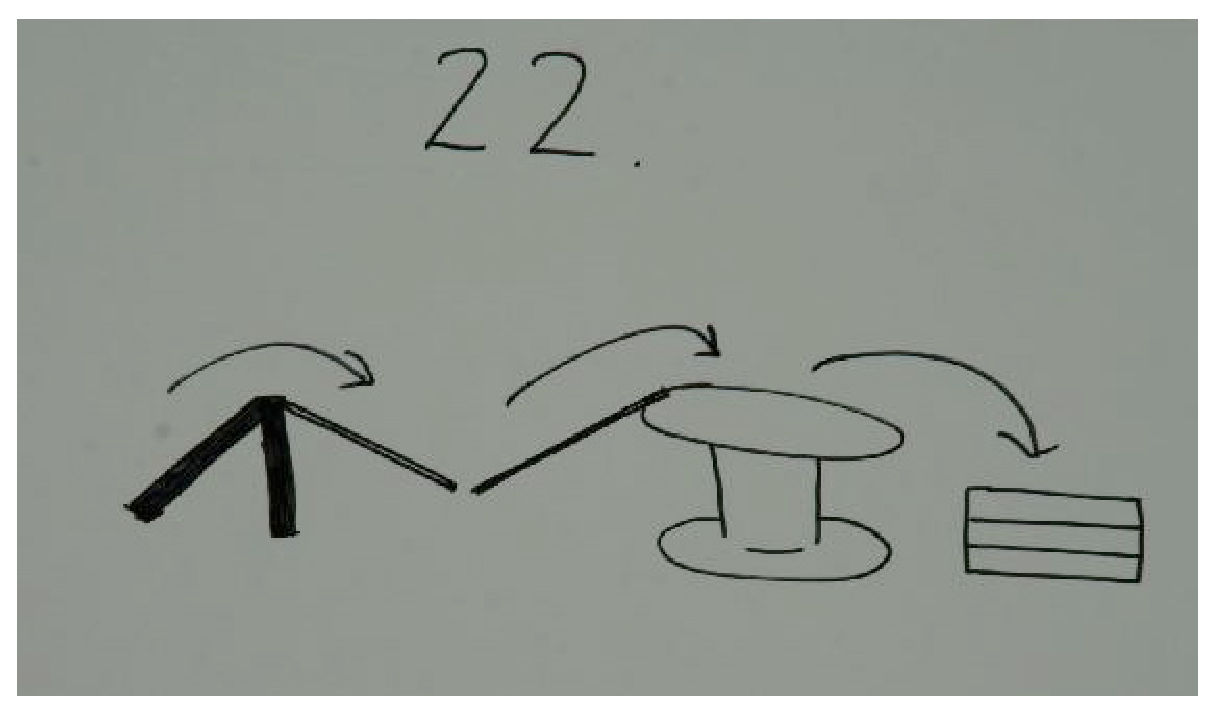
\includegraphics[scale=0.3]{trials} }\\
\hline
\end{tabular}

To make it easier to describe sections, label major obstacles with numbers and/or letters. 
These should be clearly visible at a distance. 
Plastic laminated cards with letters or numbers are good because they can be re-used at other competitions.

One good strategy is to label all boxes with numbers, and all beams with letters. 
This makes it much easier to include section descriptions such as ``ride from Beam A to Box 6, without touching the ground.''
Section instructions should not require or prohibit a rider from using certain techniques to complete a section. 
For example, the instructions must not prohibit the use of pedal grabs or bash guards in order to increase the challenge.

\subsection{Section Difficulty}
The range in difficulty of sections should correspond to the range in ability levels of the participants. 
The easiest sections should be cleanable by all participants after one or two attempts, and the harder sections should require multiple attempts by the best riders.

It is highly recommended to include one or two sections that are so difficult that they may only be cleaned by one rider, or not at all. 
This will help prevent ties for first place, and may also help to increase the technical standards of the sport if a rider succeeds in doing something that has never been done before.

\subsection{Assigning Difficulty Ratings to Sections \label{subsec:trials_guidelines-for-course-setters_assigning-difficulty-ratings}}
Assigning difficulty ratings to sections is optional, except if required to set section restrictions for competition categories (see section \ref{sec:trials_section-restrictions-for-competition-categories}).
However it is recommended as it helps riders plan which sections they want to attempt. 
The most important responsibility when assigning difficulty ratings is to be consistent.
For this reason it is best to assign difficulty ratings after all sections have been built.
Course setters should also try not to let their own strengths and limitations at different techniques bias their judgment of score values.
This is especially important for rating sections that have similar difficulty levels but that require different skills (for example: hopping, riding narrow beams, pedal grabs, etc.). 
The sections can be sorted into ``green'' (easier), ``blue'' (mid-range), and ``black'' (harder).
Each line should be marked clearly with one of these colors so that it can be seen at a distance.
If possible, the same color scheme should be shown on the rider's scoring card to make it easier for the riders to find sections of particular difficulty levels.

Two alternative methods can be used to assign ratings:

\textbf{Relative Method:}
For the purpose of grouping obstacles by difficulty, the difficulty ratings can be assigned relative to other sections in the course. A typical course would have 25\% green lines, 50\% blue lines and 25\% black lines.

\textbf{Absolute Method:}
Experienced course setters may assign Green, Blue, and Black lines based on absolute ratings of difficulty levels.
The U-System, the open-ended difficulty rating system for unicycle trials, should be used to apply ratings.
Note that the the U-system is NOT the same as the International Unicycling Federation (IUF) Skill Levels.
Because the U-system is open-ended and based on rider consensus, description of reference obstacles is outside the scope of the IUF Rulebook.
For information on the U-System, visit www.krisholm.com/u-system.

Difficulty levels can be grouped as follows:

Green lines: U0 – U2

Blue lines: U3 – U6 

Black lines: U7 and harder

In addition to assigning Green, Blue, and Black groupings, experienced course setters may wish to label each obstacle with a U-rating.
It may be helpful to rate all obstacles first, and then use this to group the obstacles by difficulty.

\subsection{Course Planning: Location And Materials}
It is most important to make maximum use of available resources. 
Prior planning and proper site selection are essential.
Expect to take at least one day to set a course for a major competition, plus time to assemble the raw building materials.

If possible, select a course location with an abundance of natural obstacles, or features that can be incorporated into human-constructed obstacles. 
It cannot be overstated that is much easier to make use of what is already there, rather than constructing new obstacles.

Sections may be set on natural features such as bedrock, boulders, logs, and hill slopes, and/or constructed from stacked pallets, railings, truck tires, junkyard cars, obstacles constructed from lumber, or any other material at hand. 
Often it is good to combine natural features with human-constructed obstacles.

It is highly recommended to also build a basic practice area to be set up outside of the competition area. 
This can consist of a small number of random obstacles, and is important for warm-up and to reduce the temptation to ride on the course prior to the event.

Make sure that there is plenty of extra building material (tools, screws, and raw materials) on hand to repair sections damaged during the event.

\subsection{Course Design}
Sections should differ substantially from each other and test a variety of hopping and rolling techniques. 
Often, it is a good idea to mentally make a list of the different techniques in trials, and design sections that test each of them separately or in combination.

The course layout is controlled mainly by the available resources.
If there are abundant natural obstacles, design sections around the most obvious natural features.

For either natural or artificial sections, a good way to maximize resources is to first construct several major structures that can be used as centerpieces, or hubs, and then design sections that center around these hubs. 
For example, a car, spool, or large boulder could serve as a hub, surrounded by smaller structures that lead onto and over the hub in different ways.

Building centralized hubs rather than independent sections allows for high concentrations of sections on less building material.
Unlike conventional bike trials, it is not a problem to design overlapping sections, although sometimes it may cause delays as riders wait for their turn. 
Usually a combination of hubs and independent sections is best.

It is extremely important to design sections that are durable enough that they do not break or change during the competition time period.

Overall, a course should not favor left or right handed riders, or riders with right- or left-foot-forward hopping stances.
For example, the Course Setter should include sections requiring hops to both the right and to the left.

It is best to design sections that provide challenge without undue risk. 
Typically the best-designed sections include moves that test balance and precision, rather than moves that are difficult only because they are big. 
For example, rather than constructing a big, basic drop or gap between easy terrain, increase the difficulty of the takeoff or landing areas by making them smaller or off-angle. 
It is strongly recommended to avoid building any drops to hard, flat ground that are greater than 1.5m height.

There is no requirement that riders exit a section while in full control of their cycle. 
Consequently, a well-designed section should force riders to be in control in order to finish---it should not be common for riders to fall across the finish line. 
The easiest way to do this is to include at least 2 meters of easy ground between the last hard obstacle and the finish line.

A photo album of previously constructed sections is located at www.krisholm.com/sections.

\subsection{Time And Space-Saving Strategies}
If building material is extremely limited and there are very few participants, an alternative competitive strategy is to create an elimination round, instead of setting an entire course.

A small number of sections are set (as little as 1 section at a time), and riders attempt all sections. 
Any rider who cannot clean an obstacle after multiple attempts is eliminated. 
Then a second set of section(s) is set, and the process repeated until only one rider can clean the section(s). 
This option works with minimal resources but should be regarded as a last resort.

\section{Multiple Rounds}
This new format is to be tested and report how it works during the next two years.

The competition is be formed by multiple rounds on the same course. 
Each round will be managed as a single trials competition. 
All other rules remain the same and each round will reset the time limit and the number of points scored. 

Each round will have a time slot and there must be at least 2 hours in between each of the rounds. 
Different rounds can be scheduled on different days.
The organizer must keep the course well built for all the time it is necessary. 
In order to improve the next round, small changes can be made to the lines during the time between rounds. 
Riders' suggestion have to be managed with attention and care, the final decision of adjusting a line is that of the main judge. 
No rider may attempt any obstacle during the time in between rounds.

The sum of the results of all the rounds determines the ranking that decides which riders will compete in the final.


\part{Hockey \label{part:hockey}}
\parttoc

\singlechapter{Hockey \label{chap:hockey}}

Attention must be drawn to the safety of the players and spectators.
Thus, the safety rules have to be obeyed strictly and all equipment must be in good condition.
These rules cannot cover every situation.
Teams have to agree on a specific amount of elbow-room before playing.
The different backgrounds of the players and the conditions of the location have to be considered.
Fairness of everyone involved is vital.

\section{Playing Field}

\subsection{Dimensions}

\begin{figure}[h]
\begin{center}
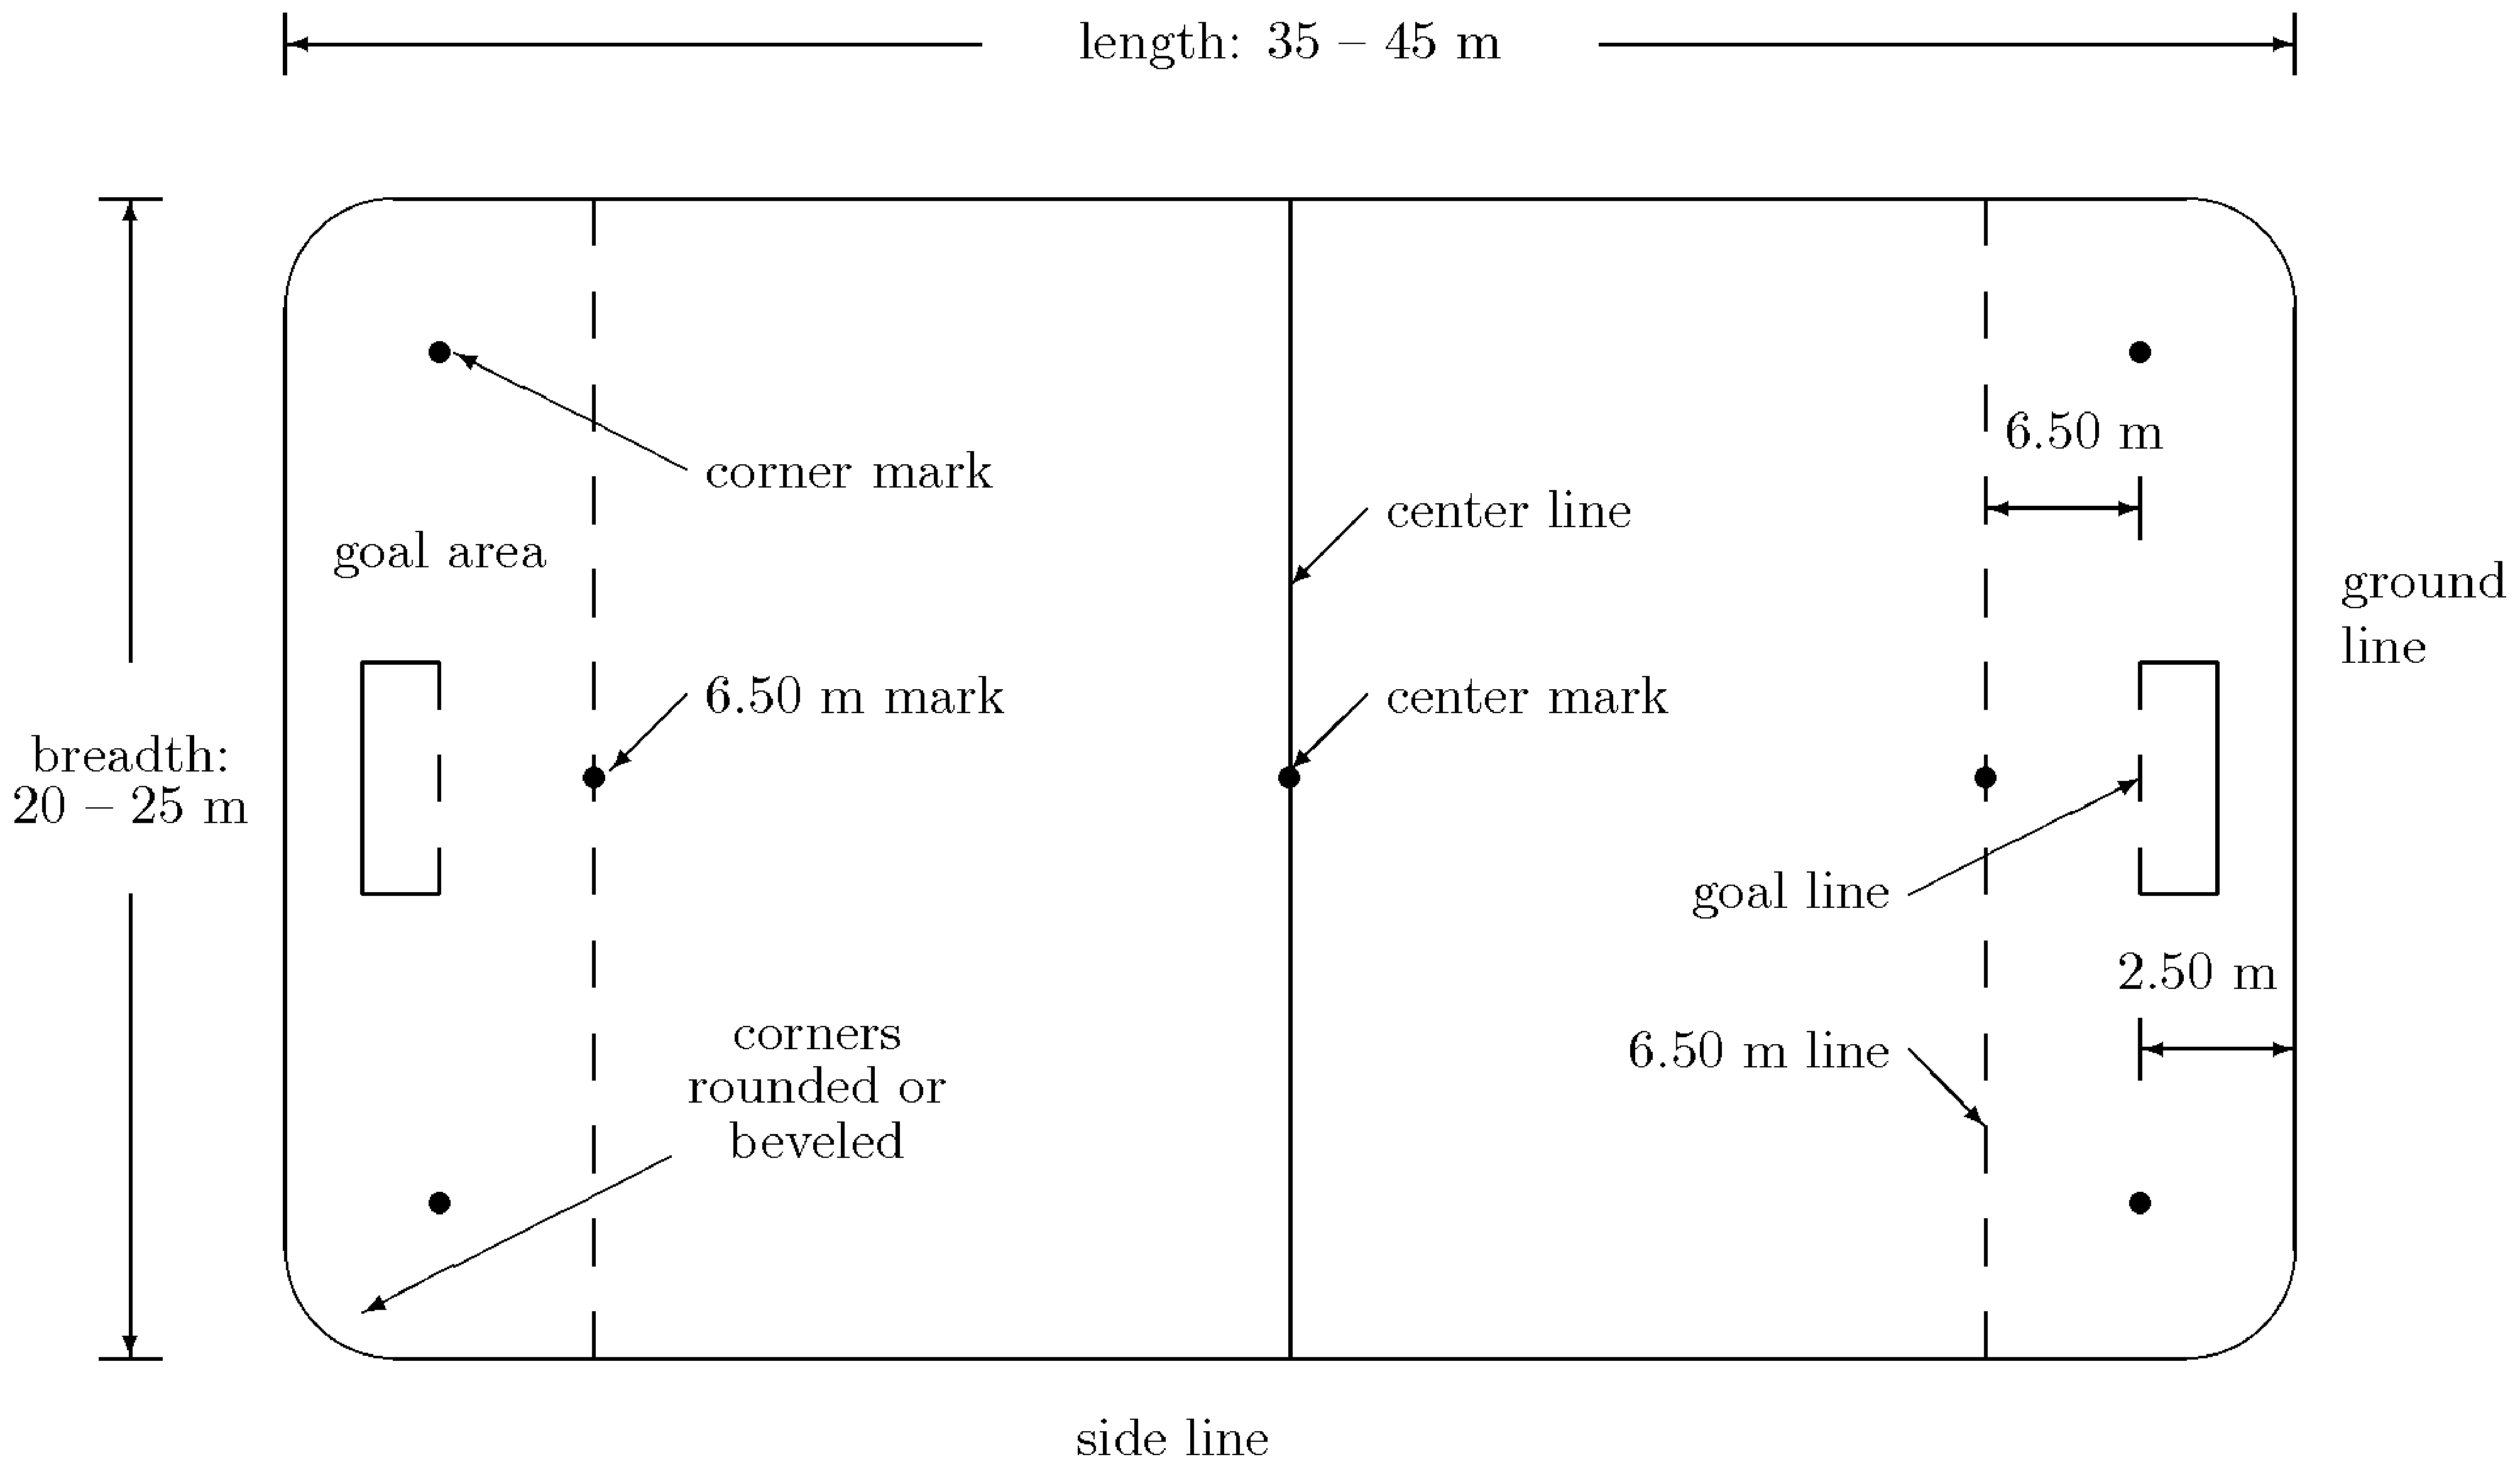
\includegraphics[scale=0.22]{dimension}
\end{center}
\end{figure}

\subsection{}
The field has a length of 35 to 45 meters and a breadth of 20 to 25 meters.
It is surrounded by barriers.
The corners are rounded or beveled.

\subsection{Goals}
The posts are 2.50 m in from the ends of the playing field (ground lines), ensuring that the players can go behind them.
The inside dimensions of goal openings are 1.20 m high and 1.80 m wide.
The goals must be made in such a way that the ball cannot enter through the rear or sides. The goals must not have sharp, pointed or protruding parts.

\subsection{Markings}
The center line divides the field into two equal halves, and the center mark is in the middle of the center line.
There are marks in front of each goal at a distance of 6.5 m.
The goal lines connect the posts on the ground.
The corner marks are on the extension of the goal lines, 1.0 m in from each side line.
The 6.5 m lines are parallel to the goal lines and run through the 6.5 m marks.
The goal areas are between the 6.5 m lines and the ends of the field.

\section{Teams}

\subsection{Number Of Players}
A team consists of five players (plus substitutes).
Substituting one player for another is possible at any time.
It is not necessary to indicate it to the Referee.
The new player must enter the field where the other exits it.
Each player can be the goalkeeper at any time.
The goalkeeper has no special rights.
To take part in a game, a team must have at least three players.

\section{Clothing}
Shoes must be worn.
All players of a team must wear shirts of the same color.
The color must be clearly different from the opponent's color.
At tournaments and other large events each team should have two different colored sets of shirts.

Clothing suggestions for comfort and safety:
\begin{itemize}
\item Cycling shorts and kneepads, or long pants
\item Gloves
\item Short shoe laces, or laces tucked in
\item Helmet and dental protection
\item Definitely no jewelry (watches, necklaces, earrings)
\end{itemize}

\section{Equipment}

\subsection{Unicycles}
The maximum wheel size is 618mm (24$"$).
The unicycles must not have sharp or protruding parts anywhere that might cause injuries.
This refers especially to quick-release levers and bolts.
The pedals must be plastic or rubber.

\subsection{Sticks}
All sticks legal for playing ice-hockey or floorball (apart from those for the goalkeeper) can be used.
Cracked or splintered sticks must be taped or repaired before play.
An upper end made of rubber is recommended.

\subsection{Ball}
A ``dead'' tennis ball that reaches 30 percent to 50 percent of its original height after bouncing onto concrete is used.
Alternatively, a street hockey ball can be used.
The choice is made by the hosting organization if the opposing teams do not agree on which ball to use.
The chosen type of ball must be announced well in advance of the competition, and must be obtainable in all participating countries.

\section{Penalties}
In every instance of a violation of the rules the Referee must penalize the offending team, unless the Referee decides not to interrupt the game (advantage).

\subsection{Free Shot}
The free shot is the standard penalty for all violations of the rules.
It is applied in all cases except for those explicitly mentioned in sections \ref{subsec:hockey_penalties_65m}–\ref{subsec:hockey_penalties_bully}.
The free shot is executed from the point where the violation was done.
\textbf{Exceptions}: If a team gets a free shot within the opponents' goal area, the free shot is done from the closest corner mark (corner shot).
If a team gets a free shot within their own goal area, the free shot is done at a distance of 1 m in front of the goal line (goalkeeper's ball).
The free shot is indirect.
The player executing the free shot may only touch the ball once.
Then another player has to touch the ball.
Opposing players must keep a distance with their unicycles and their sticks of at least 2.0 m from the ball.

\subsection{6.5 M \label{subsec:hockey_penalties_65m}}
If legal playing would have led to a direct chance to score a goal, a ``6.5 m'' is given.
This includes fouls outside the goal area.
The ball is placed at the 6.5 m mark.
A player of the defending team goes to the goal and must sit with the bottom of the wheel of their unicycle within 0.5 m of the goal line.
The other team chooses a player to shoot the 6.5 m.
All other players must leave the goal area.
After the Referee's whistle the goalkeeper must ride the unicycle freely and not rest on the goal.
If no goal is scored, play continues as soon as the ball touches the post, the keeper touches the ball or the ball crosses the extended goal line.

\subsection{Penalty Goal}
If the defending team prevents a goal from being scored through an illegal play of the ball and if, in the opinion of the Referee, the ball was traveling directly toward the goal and would definitely have entered the goal without being touched by another player, a penalty goal may be awarded.
In this case the attacking team is awarded a goal.
If there is any doubt as to the certainty of a goal, a 6.5 m must be awarded as described in section \ref{subsec:hockey_penalties_65m}.

\subsection{Bully \label{subsec:hockey_penalties_bully}}
Whenever the game needs to be resumed without penalizing one of the teams, this is done with a bully (face off).
For the bully, the Referee drops the ball between two opposing players.
Playing starts when the ball touches the ground.
A bully during the game is executed where the ball was when the game was interrupted. 
Exception: Within the goal area, the bully is always executed near one of the corner marks.

\subsection{Penalty Box}
The Referee can send a player off the field for two minutes, five minutes or for the remainder of the game.
This is done in the case of unsporting behavior and also for intentional or dangerous disregard of the rules.
While a player is in the penalty box, the team may not substitute a replacement for that player.

\section{Course Of The Game}

\subsection{Game Duration}
The play time is given by the playing schedule.
It is a relative play time.
The time only stops if the Referee requests a time out.
The teams change sides during the break.
At the start of each period, all players must be in their own half of the field.
Each period starts with a bully at the center mark.
If the game ends in a draw and a decision is necessary, play is continued for ten more minutes: five-minute break and change sides, five minutes of play, change sides without a break and five more minutes of play.
If it's still a draw, a decision is reached with a penalty shootout.

\subsection{Penalty Shootout}
Three of the players from each team get one penalty shot each.
If it is still a draw, each team shoots one more penalty until there is a decision.
It is possible that one player can make more than one shot.
However, in all cases at least two other players have to make a shot before the same player can shoot again.

For the penalty, all players except for a defending goalkeeper leave the corresponding half of the playing field.
The goalkeeper must be close to the goal line, at least until the attacking player has had contact with the ball.
The Referee places the ball on the center point and the player taking the shot will, after the whistle of the Referee, play the ball from there, trying to score a goal.
The ball must be kept in motion towards the goal line (no backwards movement allowed) and once it is shot, the play shall be considered complete.
No goal can be scored on a rebound of any kind (an exception being the ball off the goal post, then the goalkeeper and then directly into the goal), and any time the ball crosses the goal line, the shot shall be considered complete.

\subsection{Riding The Unicycle}
The player has to be riding the unicycle freely.
He or she may use the stick as support but must not rest on the goal or the wall or something similar.
It is not sufficient to release the goal only quickly for the time while the goalkeeper takes part in the game.
A short support on the wall to avoid a dismount can be tolerated.
A player who is falling off the unicycle may take part in the game until touching the ground.
A remounting player must sit on the seat and have both feet on the pedals before participating in the game again.
If a player who is not riding a unicycle shoots into their own goal, the advantage rule applies for the attacking team and the goal is valid.

\subsection{Obstacle}
A player who is off the unicycle must not be an obstacle for opponents.
The player is considered an obstacle if the player, the unicycle or stick is hit by the ball and also if an opponent cannot move around freely.
The player should remount at the same spot, but if necessary move out of the way of play first.

\subsection{Contact With The Ball}
The stick, the unicycle and the whole body can be used to play the ball.
It all counts as a contact.
Players are allowed to play the ball with the body twice in a row only if one of the contacts is passive.
When the ball is played with the body, the player must not catch or otherwise hold the ball and the contact with the ball should be instantaneous.
For arms and hands see also section \ref{subsec:hockey_goal-shots_with-arms-or-hands}.

\subsection{Start and Stop}
Starting and resuming the game is always initiated by the Referee's whistle.
When the Referee blows the whistle during the game, it is interrupted immediately.

\subsection{Restart After A Goal}
After a goal, the non-scoring team gets the ball.
All players must go to their own half.
After the Referee's whistle, the game resumes when the ball or a player of the team in possession crosses the center line.
It is legal to directly shoot a goal after passing the center line, for example without passing the ball to another player first.

\subsection{Ball Out Of Bounds}
If the ball leaves the field, the team opposite to that of the player who last touched it gets a free shot or a corner shot, depending where the ball went out.
The free shot is done 1.0 m in from the side line.

\subsection{Moving The Goal}
If a player moves the goal, the game is interrupted and the opposing team gets a free shot.

\subsection{Ball In Spokes}
If the ball gets stuck between the spokes of someone's unicycle, the opposing team gets a free shot (not a 6.5m penalty).

\section{Fouls}

\subsection{General Considerations}
All players must take care not to endanger others.
The game is contactless: the opponents and their unicycles may not be touched.
The players must take care not to hit an opponent with their stick, especially after a shot.
Only in the vicinity of the ball, they may touch an opponent's stick with their stick to block them.
However, this contact may not be hard.
It is illegal to turn the blade of the stick upside down in order to hook into an opponent's stick.
Raising the opponent's stick is allowed in principle, if not done using exaggerated roughness.
If the opponent's stick is raised above the height of their hips, it is always considered exaggerated roughness.

\subsection{Right Of Way}
To keep the game going, rule violations that do not influence the course of the game should not be penalized.
The following rules apply when riders come into contact with each other:
\begin{itemize}
\item No player may endanger another player by forcing them to give way (for example, to push them toward the wall).
\item A player who is idling or resting on the stick must be evaded.
\item The leading of two players riding next to each other may choose the direction of turns. If both are evenly side-by-side, the one having the ball may choose the direction.
\item If two players are approaching each other directly or at an obtuse angle, the one with the ball has the right of way.
\item In all cases not mentioned above, it is up to the Referee to make a decision.
\end{itemize}

\subsection{SUB (Stick Under Bike)}
A player who holds his or her stick in a way that someone else rides over or against it is committing a foul, regardless of intention.
According to the situation the player who was ``subbed'' is given either a free shot or a 6.5 m.

\subsection{SIB (Stick In Bike)}
If a stick gets into the spokes of an opponent, the holder of the stick is committing a foul regardless of intention.
According to the situation the player who was ``sibbed'' is given a free shot or a 6.5 m.

\subsection{Insults}
A player must not insult the Referee or other players.

\subsection{Intentional Fouls \label{subsec:hockey_fouls_intentional-fouls}}
Intentional fouls are considered to be unsporting behavior.
The respective player is sent off the field for at least 2 minutes.

\section{Goal Shots}

\subsection{Goal Shot With Arms Or Hands \label{subsec:hockey_goal-shots_with-arms-or-hands}}
A goal is disallowed if scored with arms or hands.
The defending team gets a free shot (goalkeeper's ball).
This rule does not apply if the ball is shot into one's own goal.

\subsection{Long Shot}
A goal is disallowed if the last contact with the ball was made when the ball was in one's own half.
The defending team gets a free shot (goalkeeper's ball).
This rule does not apply if the ball is shot from the opponents' half into one's
own goal.

\subsection{Ball In The Outside Of The Net}
If the ball becomes lodged in the outside of the goal net, or if the ball entered the goal through the net from the side the back through a hole in the net, a free shot is given against the team whose player last played the ball.

\section{Safety Rules}

\subsection{Throwing Sticks}
A player who intentionally drops or throws his or her stick is sent off the field for at least 2 minutes, at the discretion of the Referee (section \ref{subsec:hockey_fouls_intentional-fouls}).
Also, the opposing team gets a 6.5 m.

\subsection{Top Of The Stick}
The upper end of the stick must always be covered with one hand to avoid injury to other players.
A brief removal of the upper hand from the stick to play the ball with that hand is acceptable provided that this is done in a safe manner.

\subsection{The Lower End Of The Stick}
The lower end of the stick must always be below the players' hips to avoid injury to other players.
\textbf{Exception:} In direct vicinity of one's own goal, the lower end of the stick can be raised as high as the crossbar of the goal.

\subsection{Exaggerated Roughness}
Exaggerated roughness can lead to injuries and must therefore be avoided.

\section{Referee Rules}

 \subsection{Members Of The Board Of Referees}
\begin{wrapfigure}{r}{0.5\textwidth}
\begin{center}
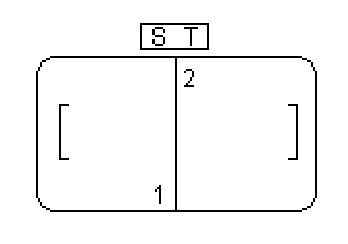
\includegraphics[scale=0.75]{referees}
\end{center}
\end{wrapfigure}
 The Board of Referees consists of:
\begin{itemize}
\item First Referee (1) 
\item Second Referee (2)
\item Secretary (S)
\item Timer (T)
\end{itemize} 

\subsection{The Referees}
The two Referees are positioned one on each side.
They try to stay close to the ball.
They should not ride a unicycle.
The clothes of the Referees must be of different color than those of the players.
Both Referees are responsible for checking all violations of the rules.
The first Referee has three additional tasks:
\begin{itemize}
\item The First Referee overrules the Second Referee, if they disagree.
\item The First Referee restarts the game after every interruption by a long blow of the whistle.
\item The First Referee drops the ball in for the bully.
\end{itemize}

\subsection{The Secretary}
The Secretary sits at the desk and takes care that the scoreboard always shows the current score.
After a goal the Secretary seeks eye contact with the First Referee to check if the goal is declared valid or not.
After the end of the game the Secretary writes the final score into the report.

\subsection{The Timer}
The Timer checks the time of play with a stopwatch.
The watch is started whenever the Referee starts the game by blowing the whistle.
At the end of each period, the Timer stops the game by blowing the whistle.
The Timer also stops the time whenever the Referee requests a time out.

\subsection{Before The Game}
Before the game, the Referees assemble all players on the field (including substitutes).
They check the following:
\begin{itemize}
\item Are the colors of the shirts of the players clearly different?
\item Did all players take off their watches and jewelry that might injure others?
\item Is the ball suitable?
\item Are the unicycles and sticks orderly, without sharp, pointed or protruding parts that might injure others?
\item They explain to the players how strictly they will interpret the rules.
\item If necessary, they tell the players how long the game will be and also if there is extended time in case of a draw.
\end{itemize}

\subsection{General}
The game is interrupted by a short and loud blow of the whistle.
If any players don't hear the whistle, it is necessary to blow the whistle again.
It is not possible to let the game continue after blowing the whistle.

The Referees should set the tone through their positive and calm appearance.
Decisions are explained upon request but they are not discussed with the players.
In an unclear situation, the Referees can ask the players before making a final decision.

Neither the Referees nor the Timer or Secretary may be distracted from the game.
Most of all, they must not talk with the spectators during the game.

If two violations of the rules occur back-to-back, only the first one is penalized.
Exception: Unsporting behavior should be penalized even after the game has been interrupted.

After a goal, the Referee waits until both teams are back in their own halves and ready to continue.
Only then, the first Referee starts the game by blowing the whistle.

If the teams start to play even though the game had not been started by the Referee, it is stopped immediately by two or more quick consecutive blows of the whistle.

To apply the advantage rule, the Referee makes the normal sign for a free shot with one arm pointing in the direction of play of the team who has the advantage.
In addition, the Referee may shout ``Advantage'' or ``Go ahead!'', but does not blow the whistle.
The end of advantage play should be signified, either by blowing the whistle to give a free shot for the original foul in the case where no advantage was gained, or by lowering the arm again and/or shouting ``Advantage over''.

After each interruption of the game the Referee briefly explains the decision.
In addition the corresponding hand sign is shown.

When two or more players fall and it is unclear whether a foul occurred, the Referees can interrupt the game and then continue it with a bully.
This prevents that even more players are drawn into the situation.

The Referees suspend the game if an injury occurs.
Afterwards, a free shot is given to the team that was in possession of the ball at the time of the interruption.
If it is unclear who was in possession, the game is continued with a bully.

\subsection{Referee Hand Signs}
\renewcommand{\arraystretch}{1.5}
\begin{longtable}{|p{3cm}|p{11cm}|}

\hline
\raisebox{-1\height}{
\includegraphics[scale=0.6]{1_h}}
&
\textbf{``Free shot''}

Point with the extended arm in the direction of play.

This sign is also used to indicate the advantage rule. \\
\hline
\raisebox{-1\height}{
\includegraphics[scale=0.6]{2_h}}
&
\textbf{``Bully''}

Hold both thumbs up.  \\
\hline
\raisebox{-1\height}{
\includegraphics[scale=0.6]{3_h}}
&
\textbf{``6.50 m''}

Point with the index finger to the 6.50 m point. \\ 
\hline
\raisebox{-1\height}{\includegraphics[scale=0.6]{4_h}}
&
 \textbf{``No Foul''}

Extend both arms horizontally.

This sign is used to indicate that there was no foul in a critical situation. It is not used in conjunction with a blow of the whistle. \\ 
\hline
\raisebox{-1\height}{
\includegraphics[scale=0.6]{5_h}}
&
\textbf{``Time out''}

Form the letter ``T'' with both hands.

The game is interrupted for example if a player is injured or if the spectators disturb the game. \\ 
\hline
\raisebox{-1\height}{
\includegraphics[scale=0.6]{6_h}}
&
\textbf{``Goal''}

Point upwards vertically with one arm.

The Referees should check here that the secretary notes the goal.
To control this it may be useful for the Referees to write down the score themselves. \\ 
\hline
\raisebox{-1\height}{
\includegraphics[scale=0.6]{7_h}}
 &
 \textbf{``No goal''}

Move the flat hand horizontally (palm pointing down).

With this hand sign a goal shot is declared invalid.
This is for example the case if the ball was last touched by hand or arm, in case of a long shot, if the ball entered the goal through the net from the outside, or if the game had already been stopped before the ball entered the goal.
The referees should check here that the Secretary does not inadvertently count the invalid goal.\\ 
\hline
\raisebox{-1\height}{
\includegraphics[scale=0.6]{8_h}}
&
\textbf{``High stick''}

Hold clenched fists next to each other above the head. \\ 
\hline
\raisebox{-1\height}{
\includegraphics[scale=0.6]{9_h}}
&
\textbf{``Penalty box for 2 minutes''}

and also 

\textbf{``Two consecutive plays with the hand''}

Spread and raise two fingers.  \\ 
\hline
\raisebox{-1\height}{
\includegraphics[scale=0.6]{10_h}}
  &
\textbf{``Penalty box for 5 minutes''}

Spread and raise five fingers.\\
\hline
\end{longtable}
\renewcommand{\arraystretch}{1}

\part{Basketball \label{part:basketball}}
\parttoc
\addstarredchapter{Basketball}
\chapter*{Basketball \label{chap:basketball}}

In IUF competition, unicycle basketball is played using the international rules for regular basketball with a few changes.
The items below, in combination with standard international basketball rules, are what are used for Unicon competition.

\section{Unicycles}
The maximum wheel size is 640mm (25.2$"$).
The unicycles must not have sharp or protruding parts anywhere that might
cause injuries.
Quick-release levers and bolts, for example, must be folded back and not excessively long.
The pedals must be plastic or rubber.

\section{Violations}
A violation occurs when the player breaks one of the rules of Basketball.
A violation results in the awarding of the ball to the opposing team.
Examples of violations include traveling, double dribble, backcourt violation, palming the ball, and stepping out of bounds.

\section{Clothing}
Shoes must be worn.
All players of a team must wear shirts of the same color.
The color must be clearly different from the opponent's color.
At tournaments and other large events each team should have two different colored sets of shirts.

Clothing suggestions for comfort and safety:
\begin{itemize}
\item Short shoe laces, or laces tucked in
\item Definitely no jewelry (watches, necklaces, earrings)
\end{itemize}

\section{Fouls}
A foul is an illegal action that can be committed by a player from one team against a player from the opposing team.
If contact occurs beyond what is deemed to be reasonable, or if a player thereby obtains an unfair advantage from it, a foul is committed.
Examples of fouls include pushing, tripping, striking or holding an opposing player and unsportsmanlike conduct.
A foul results in the awarding of the ball to the opposing team and/or free throws.

\section{Steps And Traveling}
A traveling violation occurs when a player holding the ball steps in excess of the prescribed limits.
A step is a half revolution of the wheel; meaning that each wheel revolution is the equivalent of two steps because pedaling with one leg only moves the wheel half a revolution.
After a player establishes a pivot foot (the bottom foot of an idle), the player may not switch the idle foot or take a step unless he begins dribbling.
If a player is in the act of passing or shooting the ball, then the player is allowed to take one full step without dribbling.

\section{Idling, Twisting and Hopping}
Idling is equivalent to the pivot foot and therefore is allowed.
Twisting, where the pedals stay at the same height, while you move the unicycle left and right is also considered your pivot foot, and therefore allowed.
The player must also stay within a one-meter radius from the point where the idling or twisting started.
A player may not hop (jump up and down repeatedly with the unicycle) while holding the ball.
Hopping while dribbling is permitted.

\section{Mounted Player}
The player can only play the ball while mounted on the unicycle.
A player has established position on the unicycle (``mounted'') when the player is sitting on the seat, with both feet on the pedals, and is not touching anything else for support.
Once a player is mounted, the player is considered mounted until some part of his body touches the ground.
The player throwing the ball inbound must be mounted.

\section{Unmounted Player}
If contact is made between the ball and an unmounted player or unicycle, the ball shall be awarded to the other team.
Referees may allow incidental contact between the ball and an unmounted player or unicycle if such contact does not disrupt the flow of the game.
An unmounted player must move himself and his unicycle out of the way as soon as possible
without disrupting the flow of play.
If not possible, the player must leave the unicycle where it lands until it can be retrieved without being disruptive.
A violation will result in an obstruction foul.

An unmounted player's unicycle is considered part of the player.
For the purposes of fouls, a stationary riderless unicycle is considered to have established position; a riderless unicycle that is moving is considered to be out of control.
Thus, if another player is hit by a moving abandoned unicycle, a foul will be called.
If an unmounted player intentionally attempts to play the ball or impede another player, a technical foul will be called.

\section{Four Second Zone}
The three-second zone becomes the four-second zone.

\section{Contact of the Ball with a Unicycle}
It is a violation for a player to intentionally strike or stop the ball with any part of his unicycle or leg, however, incidental contact with a player's unicycle or legs is not a violation.
As long as the player is in contact with the unicycle, riding or not, it is considered part of a player when a ball bounces out of bounds off the unicycle.
If this happens the other team receives possession of the ball.

\section{Ball on Floor}
Any player may pick up a ball that is rolling or stopped on the ground.
This can be dangerous, so care must be taken not to foul a player that is bent over to pick up the ball.
A player may stop a rolling ball with their hand or push a stopped ball to a teammate to pick up.

\newpage

\section{Referee Signals}

\textbf{Administrative signals:}

\begin{figure}[h]
\includegraphics[scale=0.6]{1-a_signal}
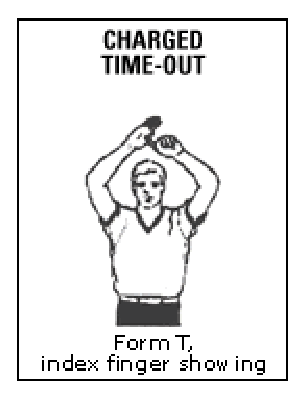
\includegraphics[scale=0.6]{1-b_signal}
\end{figure}

\textbf{Scoring signals:}
\begin{figure}[h]
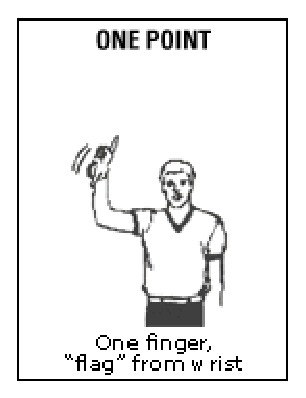
\includegraphics[scale=0.6]{2-a_signal}

\includegraphics[scale=0.6]{2-b_signal}
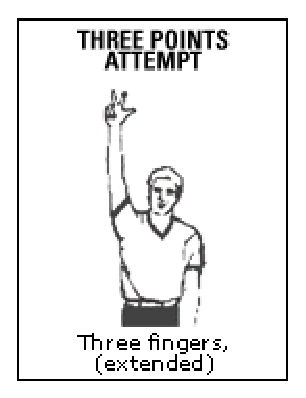
\includegraphics[scale=0.6]{2-c_signal}
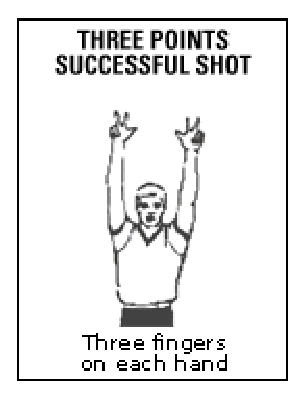
\includegraphics[scale=0.6]{2-d_signal}
\end{figure}

\textbf{Violation signals:}

\begin{figure}[h]

\includegraphics[scale=0.6]{3-a_signal}

\includegraphics[scale=0.6]{3-b_signal}

\includegraphics[scale=0.6]{3-c_signal}

\end{figure}



\backmatter
\part{Credits}

This rulebook would not exist without the work by hundreds of volunteers over the past 25 years.
We would like to recognize the volunteers since 2004.

\section{Editors and Publishers}
Constance Cotter,
Felix Dietze,
John Foss,
Thomas Gossman,
Olaf Schlote,
Rocco Schulz,
Tomislav \u{S}oi\'{c},
and Scott Wilton.

\section{Committee}

Past committee and subcommittee heads are in bold.

Heiko Allmandinger,
Jesper Andersen,
Yuta Ando,
Julia Belk,
\textbf{Klaas Bill},
Pierre-Yves Billette,
Rosi Bongers,
Franz Brandl,
Uwe Brock,
David Buchanan,
Arthur Caron,
Stephen Coleman,
\textbf{Andy Cotter},
\textbf{Constance Cotter},
Myriam Courtemanche,
Tom Daniels,
Felix Dietze,
Stephanie Dietze,
Franziska Drechsler,
Hugo Duguay,
Robin Dunlop,
Joe Dyson,
Lutz Eichholz,
Moritz Eisbach,
\textbf{John Foss},
Akiko Fujii,
Yuka Fujimoto,
Reiner F\"{u}rst,
Annette Gajowczyk,
Matthias Gauler,
Irene Genelin,
Diane Gilbertson,
Kevin Gilbertson,
Kirsten Goldstein,
Benoit Gonneville Damme,
Thomas Gossmann,
Benjamin Guiraud,
Loic Guiraud,
Marc Haefliger,
Moritz Hahn,
Helle Hartvig,
Kirsten H\"{a}usler,
Gaby Heer,
Susanne Helten,
Spencer Hochberg,
\textbf{Kris Holm},
Bj{\o}rn Hallstein Holte,
Christian Hoverath,
Carl Hoyer,
\textbf{Christian Huriwai},
Lujianne Hwang,
Kreuzer Ingrid,
Barbara Jorg,
Sayaka Kan,
Takanobu Kawamura,
Seisuke Kobayashi,
Stephan Kober,
Nina K\"{o}ning-Romswinkel,
Elke K\"{o}rner,
Adam Kover,
Dave Krack,
\textbf{Sam La Hood},
Bernd Lawrenz,
Jana Lehnert,
Pierre Letellier,
Emma Liisberg,
Fröhlin Lilo,
Jan Logemann,
Ken Looi,
Lars Lottrop,
Jonathan Marshall,
Ryohei Matsuda,
Haruko Matsunaga,
Satoko Matsunaga,
Deguti Mayuko,
Kevin McMullin,
Carlos Medina,
Tony Melton,
Yves M\'{e}try,
Sarah Miller,
Jamey Mossengren,
Barbara Niedner,
Katia Nielsen,
Nimrod Nir,
Erik Nygaard,
Hiroaki Okayama,
Yuichi Ono,
Magnus Paaske,
Mike Padial,
\textbf{Gregor Paul},
Maxime Peabody,
Sophia Pellmann,
Mike Penton,
Magnus Petersen-Paaske,
Jogi Pfender,
Petra Plininger,
Lisa Ploner,
Aurora Radavelli,
AnneSophie Rodet,
Andreas Rodler,
Daniela Ruedel,
Niels Rytter,
Satomi Sakaino,
Mayumi Sakaino,
\textbf{Rolf Sander},
Christoph Scheneker,
Marie Schlenker,
\textbf{Olaf Schlote},
Carsten Schmidt,
Marco Schmidt,
Timo Schneider,
Peter Schuhmachedr,
\textbf{Rocco Schulz},
Ayumi Sekine,
Paul Selwood,
Kaito Shoji,
Hiroyuki Shoji,
Matej \u{S}imuni\'{c},
Martin Sjönneby,
Tomislav \u{S}oi\'{c},
Kristian Sommer,
\textbf{Jim Sowers},
Virginia Steinhagen,
Reiko Suzuki,
Kyoko Takada,
Kawamura Takanobu,
Pedro Tejada,
Peter Theeg,
Arne Tilgen,
Mitsuru Tokutake,
Leo Vandewoestijne,
Marco Vitale,
Sam Wakeling,
Chris Wallace,
Nadine Wegner,
David Weichenberger,
Simon Wells,
Dana Wigert,
\textbf{Scott Wilton},
Ryan Woessner,
and
Rami Yannay.

\end{document} % Have to typset (ctrl-t) twice (or three times) to get everything to work
